\documentclass[12pt, a4paper, oneside]{book}

% --- LINGUA E CODIFICA ---
\usepackage[utf8]{inputenc}
\usepackage[T1]{fontenc}
\usepackage[italian]{babel}
\renewcommand{\familydefault}{\sfdefault} % Sans-serif moderno

\usepackage{mdframed}

% --- MARGINI E GEOMETRIA ---
\usepackage[a4paper, margin=2.5cm]{geometry}
\usepackage[export]{adjustbox}

% --- COLORI E LINK ---
\usepackage{xcolor}
\definecolor{azzurrino}{HTML}{0D47A1}
\definecolor{grigiochiaro}{HTML}{F5F5F5}
\definecolor{grigioscuro}{HTML}{424242}
\definecolor{keywordcolor}{RGB}{128, 0, 128} % Viola
\definecolor{backcolor}{RGB}{245, 245, 245}  % Grigio chiaro sfondo
%altra opzione: 1A237E



\usepackage[
    colorlinks=true,
    linkcolor=grigioscuro,
    citecolor=azzurrino,
    urlcolor=azzurrino
]{hyperref}

% --- TITOLI MODERNI ---
\usepackage{titlesec}

\titleformat{\chapter}[display]
  {\normalfont\Huge\bfseries\color{azzurrino}}
  {\filleft\Huge\thechapter}
  {0pt}
  {\titlerule[1pt]\vspace{1ex}\filright}
  [\vspace{1ex}\titlerule]

\titleformat{\section}
  {\normalfont\Large\bfseries\color{azzurrino}}{\thesection}{1em}{}

\titleformat{\subsection}
  {\normalfont\large\bfseries\color{grigioscuro}}{\thesubsection}{1em}{}

\setcounter{tocdepth}{4}
\setcounter{secnumdepth}{4}

\titleformat{\subsubsection}
  {\normalfont\large\bfseries\color{grigioscuro}}{\thesubsubsection}{1em}{}

\titleformat{\paragraph}
  {\normalfont\normalsize\bfseries\color{grigioscuro}}{\theparagraph}{1em}{}

\setcounter{tocdepth}{4}
\setcounter{secnumdepth}{4}

% --- CAPTION COLORATE ---
\usepackage[font=small, labelfont={bf, color=azzurrino}]{caption}

% --- HEADER E FOOTER ---
\usepackage{fancyhdr}
\setlength{\headheight}{25pt}
\pagestyle{fancy}
\fancyhf{}
\fancyhead[L]{\color{grigioscuro}\leftmark}
\fancyhead[R]{\color{azzurrino}\thepage}
\renewcommand{\headrulewidth}{0.4pt}
\renewcommand{\headrule}{\hbox to\headwidth{\color{azzurrino}\leaders\hrule height \headrulewidth\hfill}}
\fancyfoot[C]{\color{grigioscuro}\small Basi di dati – \thepage}

% --- LISTE ED ENUMERAZIONI ---
\usepackage{enumitem}
\setlist{nosep, leftmargin=1.5em}

% --- GRAFICA E FIGURE ---
\usepackage{graphicx}
\usepackage{bookmark}
\usepackage{float}
\usepackage{wrapfig}
\usepackage[normalem]{ulem} % sottolineature
\usepackage{subcaption}
\usepackage{soul} % evidenziazione
\usepackage{parskip} % spaziatura tra paragrafi
\usepackage{tikz}
\usepackage{cancel}

% --- Tcolorbox e Listings ---
\usepackage[most]{tcolorbox}
\tcbuselibrary{listings, skins, breakable, theorems} % theorems utile per ambienti come erexercise
\usepackage{amsmath}
\usepackage{amssymb}
\usepackage{textcomp}
\usepackage{listings}

% --- Tabelle ---
\usepackage{longtable}
\usepackage{multirow}
\usepackage{array}
\usepackage{tabularx}

% --- FRONTESPIZIO ---
\title{\Huge\bfseries Appunti del corso di \\[0.5ex]
\textcolor{azzurrino}{Basi di dati} \\[1ex]
\Large UniVR - Dipartimento di Informatica \\[1.5ex]
\Large secondo semestre - A.A. 2025/26}
\author{\bfseries \Large \textcolor{azzurrino}{Mattia Nicolis} \and \bfseries \Large \textcolor{azzurrino}{Matteo Drago}}
\date{}

% --- DEFINIZIONE DI AMBIENTI DI LAVORO ---
%===========================================
% --- AMBIENTE DEFINIZIONE ---
\newcommand{\definizione}[2]{%
  \vspace{5pt}%
  \begin{tcolorbox}[
    colback=azzurrino!5!white,
    colframe=azzurrino!50!black,
    title=\textbf{Definizione: #1},
    coltitle=white,
    fonttitle=\bfseries,
    arc=2mm,
    boxrule=1pt,
    enhanced,
    breakable
  ]
  #2
  \end{tcolorbox}
  \vspace{5pt}%
}

% --- AMBIENTE DEFINIZIONE (Viola) ---
\newcommand{\Definizione}[2]{%
  \vspace{5pt}%
  \begin{tcolorbox}[
    colback=viola!5!white,
    colframe=viola!50!black,
    title=\textbf{Definizione: #1},
    coltitle=white,
    fonttitle=\bfseries,
    arc=2mm,
    boxrule=1pt,
    enhanced,
    breakable
  ]
  #2
  \end{tcolorbox}
  \vspace{5pt}%
}

% --- AMBIENTE DEFINIZIONE (Verde) ---
\newcommand{\definition}[2]{%
  \vspace{5pt}%
  \begin{tcolorbox}[
    colback=verde!5!white,
    colframe=verde!50!black,
    title=\textbf{Definizione: #1},
    coltitle=white,
    fonttitle=\bfseries,
    arc=2mm,
    boxrule=1pt,
    enhanced,
    breakable
  ]
  #2
  \end{tcolorbox}
  \vspace{5pt}%
}

%===========================================
% --- AMBIENTE ESEMPIO ---
\newcommand{\esempio}[2]{%
  \vspace{5pt}%
  \begin{tcolorbox}[
    colback=brown!5!white,
    colframe=brown!50!black,
    title=\textbf{Esempio: #1},
    coltitle=white,
    fonttitle=\bfseries,
    arc=2mm,
    boxrule=1pt,
    enhanced,
    breakable
  ]
  #2
  \end{tcolorbox}
  \vspace{5pt}%
}

%===========================================
% --- AMBIENTE VARIO ---
\newcommand{\vario}[2]{%
  \vspace{5pt}%
  \begin{tcolorbox}[
    colback=orange!10!white,
    colframe=orange!70!black,
    title=\textbf{#1},
    coltitle=white,
    fonttitle=\bfseries,
    arc=2mm,
    boxrule=1pt,
    enhanced,
    breakable
  ]
  #2
  \end{tcolorbox}
  \vspace{5pt}%
}

%===========================================
% --- STILI PER I LINGUAGGI DI PROGRAMMAZIONE ---
%===========================================
\lstdefinestyle{Rstyle}{
  language=R,
  basicstyle=\ttfamily\small,
  keywordstyle=\color{blue},
  stringstyle=\color{red},
  keepspaces=true,       % <-- Rispetta gli spazi
  columns=fixed,  % <-- Impedisce a LaTeX di allargare il testo
  commentstyle=\color{green!50!black}, % NESSUN CANCELLETTO QUI, ERRORE RISOLTO!
  morekeywords={c, length, print, summary, mean, sd, var, min, max, sum, 
                seq, rep, paste, paste0, rbind, cbind, matrix, data.frame, 
                list, str, class, typeof, apply, lapply, sapply, tapply, 
                plot, hist, boxplot, read.csv, write.csv, head, tail, 
                subset, merge, table, ifelse, require, install.packages, library},
  numbers=left,
  numberstyle=\tiny\color{gray},
  breaklines=true,
  showstringspaces=false
}

\lstdefinestyle{SQLstyle}{
  language=SQL,
  basicstyle=\ttfamily\footnotesize,
  keywordstyle=\color{keywordcolor}\bfseries,
  commentstyle=\color{gray},
  stringstyle=\color{red},
  breaklines=true,
  showstringspaces=false,
  morekeywords={DISTINCT, AS, FROM, WHERE, GROUP, BY, HAVING, UNION, INTERSECT, EXCEPT, ORDER, ASC, DESC, USING}
}

\lstdefinestyle{Javastyle}{
  language=Java,
  basicstyle=\ttfamily\footnotesize,
  keywordstyle=\color{viola}\bfseries,
  stringstyle=\color{red},
  commentstyle=\color{green!60!black}\itshape,
  breaklines=true,
  showstringspaces=false
}

%===========================================
% --- AMBIENTI CODICE (SENZA TITOLO) ---
%===========================================
\newtcblisting{codiceR}[1][]{%
  width=\linewidth, % <--- AGGIUNGI QUESTA RIGA!
  colback=yellow!10!white,
  colframe=yellow!50!black,
  sharp corners, % <-- Angoli vivi, zero arrotondamenti
  boxrule=0.8pt,
  top=0pt,       % <-- Rimuove la riga vuota interna superiore
  bottom=0pt,    % <-- Rimuove la riga vuota interna inferiore
  left=2pt,      % Un minimo indispensabile per non appiccicare le lettere al bordo
  right=2pt,
  enhanced,
  breakable,
  listing only,
  listing options={style=Rstyle}, 
  #1 
}

\newtcblisting{codiceSQL}[1][]{%
  colback=blue!3!white,     % Azzurrino chiarissimo
  colframe=blue!40!black,   % Bordo blu neutro
  arc=2mm,
  boxrule=0.8pt,
  enhanced,
  breakable,
  listing only,
  listing options={style=SQLstyle},
  #1
}

\newtcblisting{codiceJava}[1][]{%
  colback=orange!5!white,   % Arancione molto tenue
  colframe=orange!60!black, % Bordo arancione bruciato
  arc=2mm,
  boxrule=0.8pt,
  enhanced,
  breakable,
  listing only,
  listing options={style=Javastyle},
  #1
}

%==========================================
% --- AMBIENTI ER E MATEMATICI ---
%==========================================
\newtcolorbox{er}[2][]{%
  enhanced, breakable,
  colback=gray!3,
  colframe=blue!50!black,
  fonttitle=\bfseries,
  title={Esercizio E-R: #2},
  before upper={\refstepcounter{erex}},
  sharp corners=south,
  boxrule=0.8pt,
  arc = 2mm,
  #1
}

\newcommand{\teorema}[2]{%
  \vspace{5pt}%
  \begin{tcolorbox}[
    colback=red!5!white,
    colframe=red!50!black,
    title=\textbf{Teorema: #1},
    coltitle=white,
    fonttitle=\bfseries,
    arc=2mm,
    boxrule=1pt,
    enhanced,
    breakable
  ]
  #2
  \end{tcolorbox}
  \vspace{5pt}%
}

\newcommand{\lemma}[3]{%
  \vspace{5pt}%
  \begin{tcolorbox}[
    colback=red!5!white,
    colframe=red!50!black,
    title=\textbf{Lemma: #1},
    coltitle=white,
    fonttitle=\bfseries,
    arc=2mm,
    boxrule=1pt,
    enhanced,
    breakable
  ]
  #2
  \ifstrempty{#3}{}{%
    \par\vspace{8pt}%
    \textbf{Dimostrazione}\\
    #3
  }
  \end{tcolorbox}
  \vspace{5pt}%
}

\newcommand{\osservazione}[1]{%
  \vspace{5pt}%
  \begin{tcolorbox}[
    colback=white!5!white,
    colframe=white!50!black,
    title=\textbf{Osservazione},
    coltitle=white,
    fonttitle=\bfseries,
    arc=2mm,
    boxrule=1pt,
    enhanced,
    breakable
  ]
  #1
  \end{tcolorbox}
  \vspace{5pt}%
}

\newtcolorbox{esempiobox}[1]{
    colback=brown!5, 
    colframe=brown, 
    title=#1, 
    fonttitle=\bfseries
} %file apposito per definire nuovi comandi


% =================================
\begin{document}
    \frontmatter
    \maketitle
    \tableofcontents
    \thispagestyle{empty}
    \newpage

    %===========================
    \mainmatter

    %-----------CAPITOLO 1: RIPASSO GENERALE DEGLI ARGOMENTI------
    \chapter{Tecnologie per le basi di dati}

    \definizione{DBMS}{
      Un \textbf{D}atabase \textbf{M}anagement \textbf{S}ystem è un software in grado di gestire collezioni di dati che siano \textcolor{azzurrino}{grandi}, \textcolor{azzurrino}{condivise} e \textcolor{azzurrino}{persistenti}, assicurando la loro \textcolor{azzurrino}{affidabilità} e \textcolor{azzurrino}{privatezza}.

      \noindent\rule{\textwidth}{0.4pt}

      \medskip
      \begin{itemize}[label=$\triangleright$, itemsep=\smallskipamount]
        \item \textbf{grandi}: dati devono essere organizzati in modo efficiente per poter essere gestiti in grandi quantità
        \item \textbf{condivise}: dati devono essere accessibili da più utenti contemporaneamente
        \item \textbf{persistenti}: dati devono essere memorizzati in modo permanente, anche dopo la chiusra del programma
        \item \textbf{affidabili}: dati devono essere protetti da errori e guasti del sistema
        \item \textbf{privati}: dati devono essere protetti da accessi non autorizzati 
      \end{itemize}
    }

    Un DBMS in quanto sistema software deve essere \textbf{efficiente} ed \textbf{efficace} e deve, inoltre, estendere le funzionalità del file system.


    \definizione{base di dati}{Una \textbf{base di dati} è una collezione di dati gestita da un DBMS.}

    \section{Architettura transazionale di un DBMS}
    Un DBMS è costituto tra 3 livelli:

    \begin{figure}[H]
      \centering
      
\includegraphics[width=0.7\textwidth]{images/schema.png}
    \end{figure}

    Un DBMS basato sul \textbf{modello relazionale} è nella maggior parte dei casi anche un sistema transazionale: fornisce un meccanismo per la definizione ed esecuzione di transazioni.

    \begin{figure}[H]
      \centering
      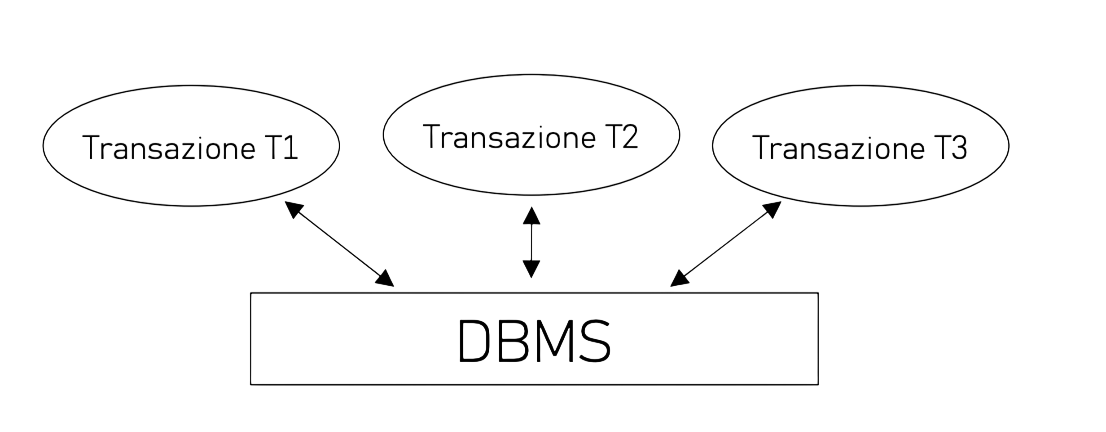
\includegraphics[width=0.9\textwidth]{images/DBMS.png}
      \caption{sistema transizionale}
    \end{figure}

    \section{Transazione}

    \definizione{Transazione}{Una \textbf{transazione} è un’unità di lavoro svolta da un programma applicativo (che interagisce con una base di dati) per la quale si vogliono garantire proprietà di correttezza, robustezza e isolamento.}

    Le caratteristiche principali sono:
    \begin{itemize}[label=$\triangleright$, itemsep=\smallskipamount]
      \item \textbf{atomicità}: una transazione  deve essere eseguita completamente o non essere eseguita affatto
      \item \textbf{non sono ammesse esecuzioni parziali}
    \end{itemize}

    \subsection{Sintassi}
    La sintassi per definire una transazione in SQL:
    \begin{sqlcode}
      <transazione> -> begin transaction
                        <programma>
                       end transaction
      
      <programma> -> < <istruzione> | commit work | rollback work >
                     { < <istruzione> | commit work | rollback work > }
    \end{sqlcode}

    La transazione va a buon fine all’esecuzione di un $\verb|commit work|$, ma non ha alcun effetto se viene eseguito un $\verb|rollback work|$.

    \medskip
    Per essere ben formata, una transazione deve:
    \begin{itemize}[label=$\circ$, itemsep=\smallskipamount]
      \item \textbf{iniziare} con un $\verb|begin transaction|$
      \item \textbf{terminare} con un $\verb|end transaction|$
      \item \textbf{esecuzione} comportare il raggiungimento di un$ \verb|commit|$ o di un $\verb|rollback work|$, a seguito del quale non si eseguono altri accessi alla base di dati
    \end{itemize}

    \begin{sqlcode}
      begin transaction;
        update CONTO set saldo = saldo - 1200
          where filiale = '005' and numero = 15;
        update CONTO set saldo = saldo + 1200
          where filiale = '005' and numero = 205;
        commit work;
      end transaction;
    \end{sqlcode}

    \subsection{Proprietà delle transazioni}
    Una transazione ha 4 proprietà fondamentali:
    \begin{enumerate}[itemsep=\smallskipamount]
      \item \textcolor{azzurrino}{\textbf{atomicità}}: una transazione è una unità di esecuzione indivisibile (viene eseguita completamente o non viene eseguita affatto).
      
      Questo implica:
      \begin{itemize}[label=$\diamond$, itemsep=\smallskipamount]
        \item se una transazione viene interrotta prima del $\verb|commit|$, il lavoro fin qui eseguito dalla transazione deve essere disfatto ripristinando la situazione in cui si trovava la base di dati prima dell’inizio della transazione
        \item se una transazione viene interrotta dopo l’esecuzione del $\verb|commit|$ ($\verb|commit|$ eseguito con successo), il sistema deve assicurare che la transazione abbia effetto sulla base di dati
      \end{itemize}
      \item \textcolor{azzurrino}{\textbf{consistenza}}: esecuzione di una transazione non deve violare i vincoli di integrità.
      
      Questo implica:
      \begin{itemize}[label=$\diamond$, itemsep=\smallskipamount]
        \item verifica immediata:
        \begin{itemize}[itemsep=\smallskipamount]
          \item fatta nel corso della transazione
          \item viene abortita solo l’ultima operazione e il sistema restituisce all’applicazione una segnalazione d’errore
          \item applicazione può reagire alla violazione
        \end{itemize}
        \item verifica differita:
        \begin{itemize}[itemsep=\smallskipamount]
          \item  al $\verb|commit|$ se un vincolo di integrità viene violato la transazione viene abortita senza possibilità da parte dell’applicazione di reagire alla violazione
        \end{itemize}
      \end{itemize}
      \item \textcolor{azzurrino}{\textbf{isolamento}}: esecuzione di una transazione deve essere indipendente dalla contemporanea esecuzione di altre transazioni
      \begin{itemize}[itemsep=\smallskipamount]
        \item $\verb|rollback|$ di una transazione non deve creare $\verb|rollback|$ a catena di altre transazioni che si trovano in esecuzione contemporaneamente
        \item  sistema deve regolare l’esecuzione concorrente con meccanismi di controllo dell’accesso alle risorse
      \end{itemize}
      \item \textcolor{azzurrino}{\textbf{persistenza}}: effetto di una transazione che ha eseguito il $\verb|commit|$ non deve andare perso
      \begin{itemize}[itemsep=\smallskipamount]
        \item sistema deve essere in grado, in caso di guasto, di garantire gli effetti delle transazioni che al momento del guasto avevano già eseguito un $\verb|commit|$
      \end{itemize}
    \end{enumerate}

    Un DBMS che gestisce transazioni dovrebbe garantire per ogni transazione che esegue tutte queste proprietà.

    \section{Architettura di un DBMS}
    L’architettura di un DBMS è composta da \textbf{moduli} che si occupano di gestire le diverse funzionalità del sistema.

    \begin{figure}[H]
      \centering
      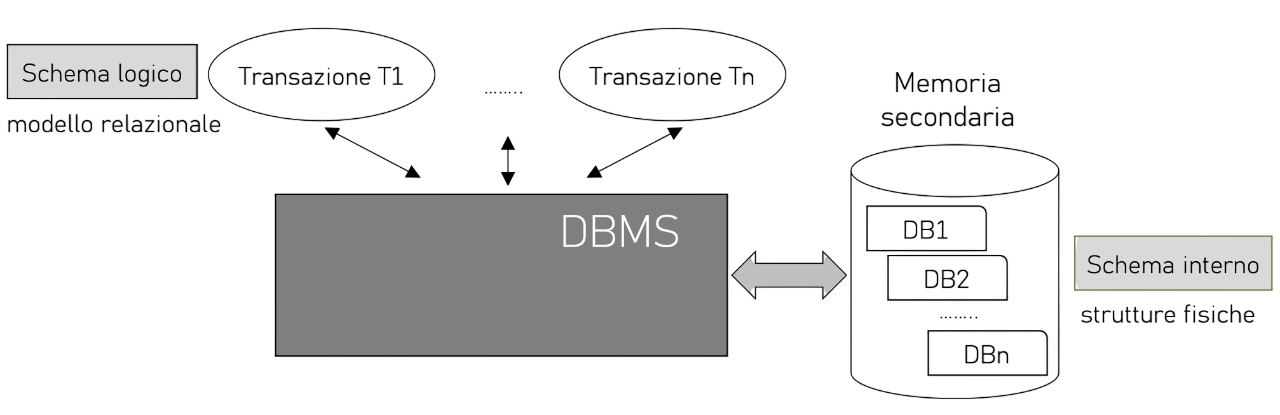
\includegraphics[width=0.6\textwidth]{images/ArchitetturaDBMS.png} 
      \caption{architettura di riferimento di un DBMS}
    \end{figure}

    Il modulo di gestione delle transazionisi occupa di trasformare una transazione in un insieme di operazioni sulla base di dati, garantendo le proprietà ACID.

    \begin{figure}[H]
      \centering
      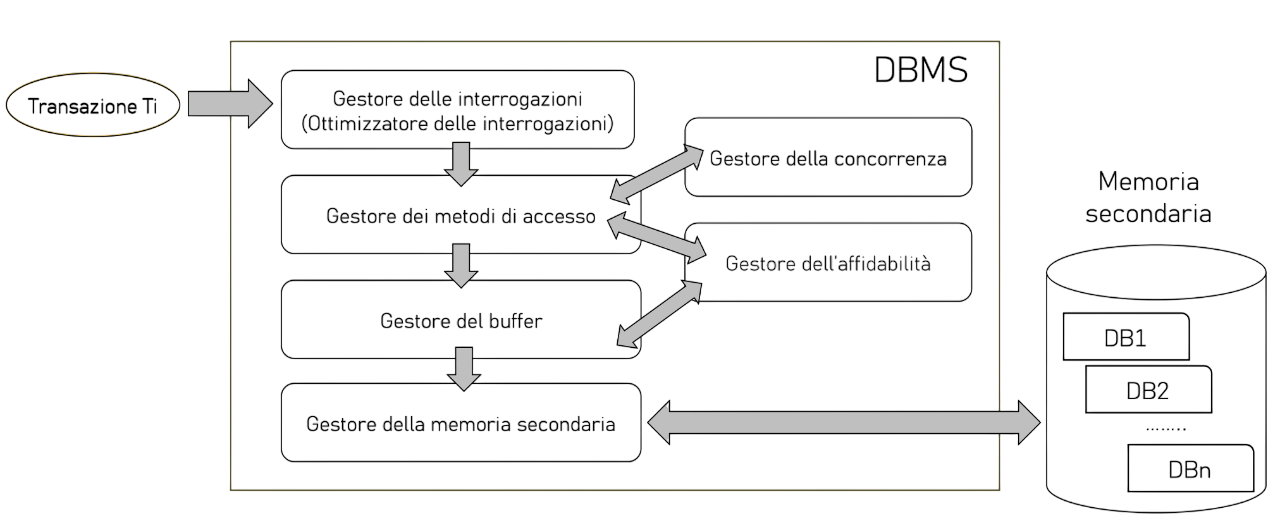
\includegraphics[width=0.6\textwidth]{images/Architettura2.png} 
      \caption{modulo di gestione delle transazion di un DBMS}
    \end{figure}

    I singoli moduli che compongono questo modulo sono:
    \begin{itemize}[label=$\triangleright$, itemsep=\smallskipamount]
      \item \textcolor{azzurrino}{\textbf{gestore delle interrogazioni}}: riceve in ingresso una query SQL
      \begin{figure}[H]
        \centering
        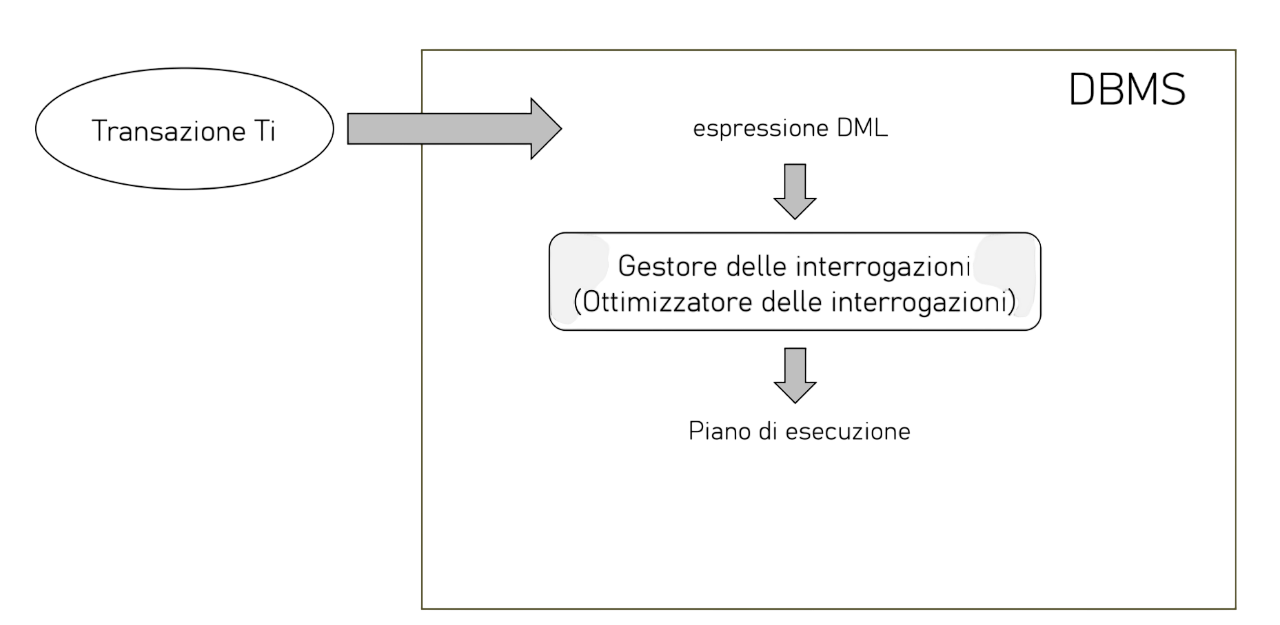
\includegraphics[width=0.6\textwidth]{images/passaggio1.png} 
      \end{figure}
      \item\textcolor{azzurrino}{ \textbf{gestore dei metodi di accesso}}: determina quali sono le pagine della memoria secondaria di cui si ha bisogno, ma capisce anche se è possibile accederci
      \begin{figure}[H]
        \centering
        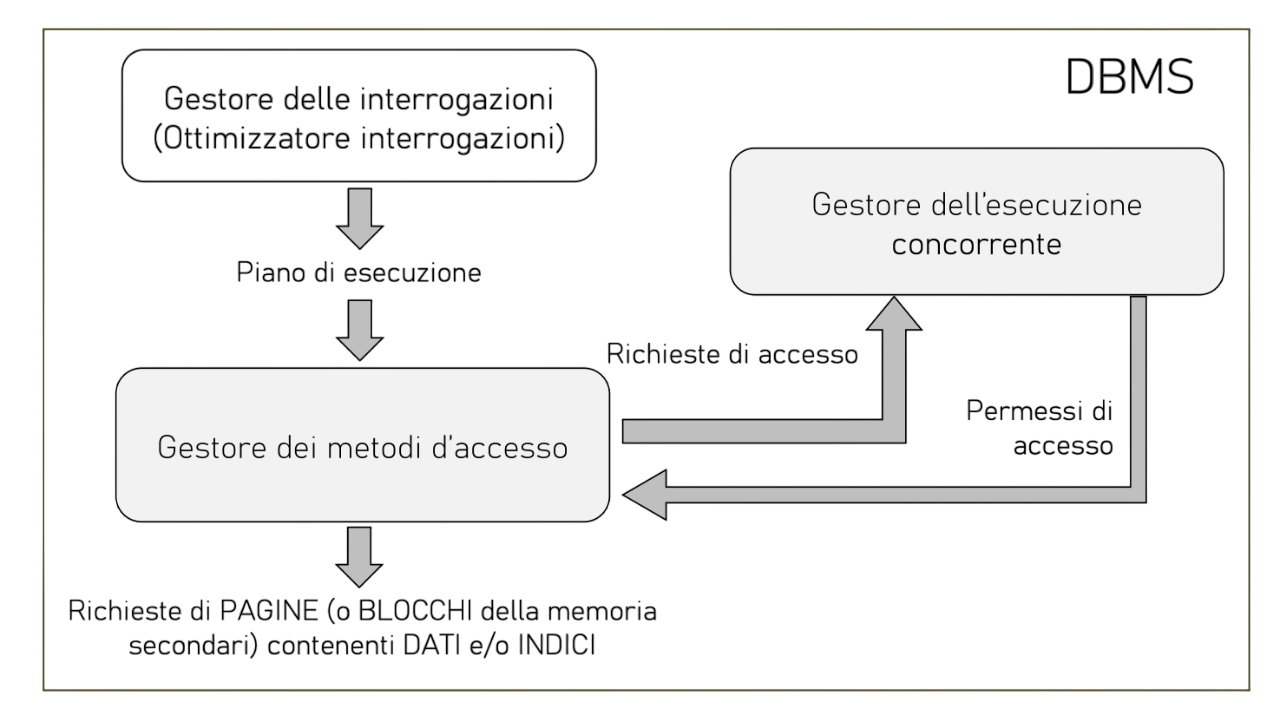
\includegraphics[width=0.6\textwidth]{images/passaggio2.png} 
      \end{figure}
      \item \textcolor{azzurrino}{\textbf{gestore dell’affidabilità}}: carica in memoria principale le pagine della memoria secondaria di cui si ha bisogno, e le mantiene in memoria finché non sono più necessarie
      \begin{figure}[H]
        \centering
        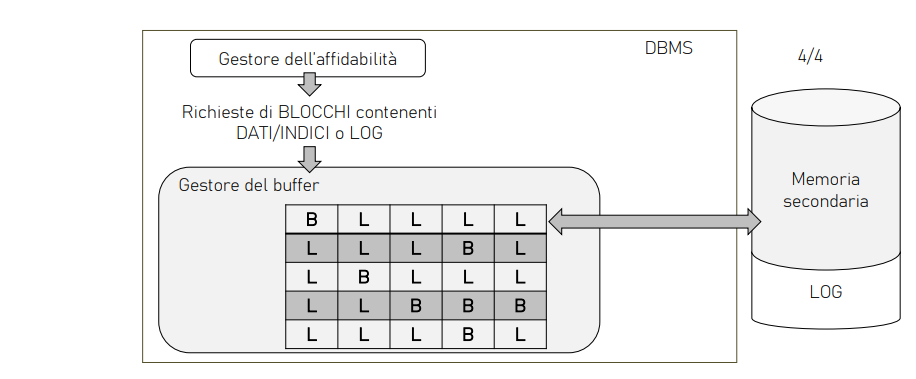
\includegraphics[width=0.6\textwidth]{images/passaggio4.png} 
      \end{figure}
      \item \textcolor{azzurrino}{\textbf{gestore del buffer}}
      \item \textcolor{azzurrino}{\textbf{gestore dell’esecuzione concorrente}}
      \item \textcolor{azzurrino}{\textbf{gestore dell’affidabilità}}
    \end{itemize}

    \bigskip
    I moduli che contribuiscono a garantire le proprietà ACID sono:
    \begin{itemize}[label=$\circ$, itemsep=\smallskipamount]
      \item \textbf{gestore dei metodi d'accesso}: consistenza
      \item \textbf{gestore dell'esecuzione concorrente}: atomicità e isolamento
      \item \textbf{gestore dell'affidabilità}: atomicità e persistenza  
    \end{itemize}


!TeX root = BasiDiDati.tex

%---------CAPITOLO 2: LINGUAGGIO SQL--------------------------------------------------
    \chapter{Linguaggio SQL}
    Il termine SQL in origine era l'acronimo di \textbf{S}tructured \textbf{Q}uery \textbf{L}enguagge, ma ad oggi è diventato un nome proprio.

    \definizione{linguaggio SQL}{
      \raggedright
      Il \textbf{linguaggio di interrrogazione SQL} permette di:
      \begin{itemize}[label=$\triangleright$, itemsep=\smallskipamount]
        \item \textbf{definire delle strutture dati e i vincoli di integrità}: \textcolor{azzurrino}{\textbf{D}}ata \textcolor{azzurrino}{\textbf{D}}efinition \textcolor{azzurrino}{\textbf{L}}enguagge
        \item \textbf{manipolare i dati} (inserimento, aggiornamento e cancellazione): \textcolor{azzurrino}{\textbf{D}}ata \textcolor{azzurrino}{\textbf{M}}anipilation \textcolor{azzurrino}{\textbf{L}}enguagge
        \item \textbf{interrogare}: \textcolor{azzurrino}{\textbf{D}}ata \textcolor{azzurrino}{\textbf{Q}}uery \textcolor{azzurrino}{\textbf{L}}enguagge
      \end{itemize}
    }

    Esistono diverse versioni:

    \begin{center}
      \begin{longtable}{|c|c|l|}
      \hline
      \textbf{Nome informale} & \textbf{Nome ufficiale} & \multicolumn{1}{c|}{\textbf{Caratteristiche}} \\ \hline
      \endfirsthead
      \hline
      \textbf{Nome informale} & \textbf{Nome ufficiale} & \multicolumn{1}{c|}{\textbf{Caratteristiche}} \\ \hline
      \endhead

      \multirow{2}{*}{SQL base} & SQL-86 & Costrutti base \\ \cline{2-3} 
                                & SQL-89 & Integrità referenziale \\ \hline
      SQL-2                     & SQL-92 & \begin{tabular}[c]{@{}l@{}}Modello relazionale\\ Vari costrutti nuovi\\ 3 livelli: entry, intermediate, full\end{tabular} \\ \hline
      \multirow{10}{*}{SQL-3}   & SQL:1999 & \begin{tabular}[c]{@{}l@{}}Modello relazionale a oggetti\\ Organizzato in diverse parti\\ Trigger, funzioni esterne, ...\end{tabular} \\ \cline{2-3} 
                                & SQL:2003 & \begin{tabular}[c]{@{}l@{}}Estensioni del modello a oggetti\\ Eliminazione di costrutti non usati\\ Nuove parti: SQL/JRT, SQL/XML, ...\end{tabular} \\ \cline{2-3} 
                                & SQL:2006 & Estensione della parte XML \\ \cline{2-3} 
                                & SQL:2008 & Lievi aggiunte (per esempio, \texttt{trigger instead of}) \\ \cline{2-3} 
                                & SQL:2011 & Ricco supporto per dati temporali \\ \cline{2-3} 
                                & SQL:2016 & Gestione del formato JSON \\ \hline
      \end{longtable}
    \end{center}

    La parte di SQL dedicata alle dichiarazioni fa parte dei DML.\\[0.2ex]
    Le dichiarazioni vengono espresse in modo dichiarativo: specifica l'obiettivo e non la procedura per ottenerlo (algebra relazionale).
    
    Una parte del DBMS, detta $\verb|query optimizer|$, traduce di fatto l’interrogazione SQL nel linguaggio procedurale interno del sistema, che è nascosto all’utente.\\[0.2ex]
    SQL permette, quindi, di descrivere le interrogazioni in modo astratto ed ad alto livello.

    \section{Istruzione \protect\texttt{SELECT}}
    La sintassi dell’istruzione $\verb|SELECT|$ è:
    \begin{sqlcode}
      SELECT [ DISTINCT ]
      [ * | expression [[ AS ] output_name ] [, ...] ]
      [ FROM from_item [, ...] ]
        [ WHERE condition ]
          [ GROUP BY grouping_element [, ...] ]
          [ HAVING condition [, ...] ]
          [ { UNION | INTERSECT | EXCEPT } [ DISTINCT ] other_select ]
            [ ORDER BY expression [ ASC | DESC | USING operator ]]
    \end{sqlcode}

    dove:
    \begin{itemize}[label=$\triangleright$, itemsep=\smallskipamount]
      \item \textbf{expression}: è un’espressione che determina un attributo
      \item \textbf{from\_item}: è un’espressione che determina una sorgente per gli attributi
      \item \textbf{condition}: è un’espressione booleana per selezionare i valori degli attributi
      \item \textbf{grouping\_element}: è un’espressione per poter eseguire operazioni su più valori di un attributo e considerare il risultato.
    \end{itemize}

    La struttura dell’istruzione è la seguente:
    \begin{sqlcode}
      SELECT attributo
      FROM tabella
        [WHERE condizione]
    \end{sqlcode}

    $\verb|SELECT|$, $\verb|FROM|$ e $\verb|WHERE|$ sono chiamate \textbf{clausole}.\\[0.2ex]
    La clausula $\verb|SELCET|$ estrae dal prodotto cartesiano delle tabelle elencate nella clausola $\verb|FROM|$, le righe che soddisfano la condizione specificata nella clausola $\verb|WHERE|$.\\[0.2ex]
    Il risultato dell‘interrogazione è una tabella con una riga per ogni riga prodotta dalla clausola $\verb|FROM|$ ed, eventualmente, filtrata dalla clausola $\verb|WHERE|$ (se esiste), le cui colonne dipendono dalla lista degli attributi nella clausola $\verb|SELCET|$.

    \begin{esempiobox}{Interrogazione con \texttt{SELECT}}
      Consideriamo la seguente base di dati:

      \begin{center}
        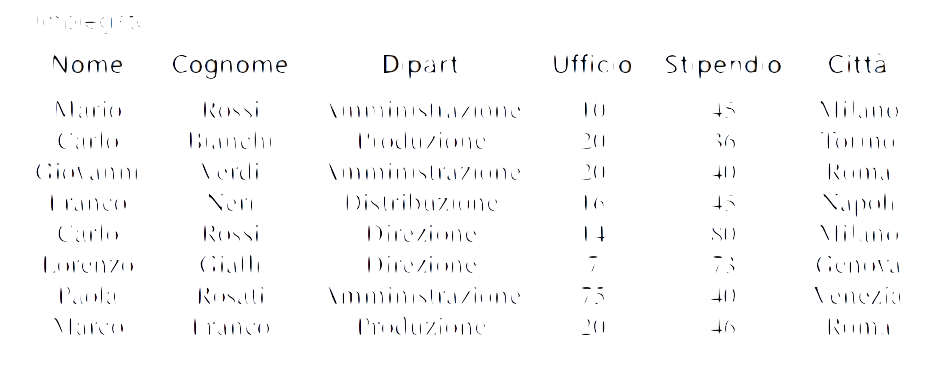
\includegraphics[width=0.5\textwidth]{images/tabella-impiegato.png}
      \end{center}
      
      \textbf{Estrarre lo stipendio degli impiegati di cognome ’Rossi’}.

      \begin{sqlcode}
        SELECT Stipendio
        FROM Impiegato
          WHERE Cognome = 'Rossi';
      \end{sqlcode}

      Il risultato dell'interrogazione è la seguente tabella:
      \begin{center}
        
\includegraphics[width=0.2\textwidth]{images/select-impiegato.png}
      \end{center}
    \end{esempiobox}

    \bigskip
    Il simbolo $\verb|*|$ permette di  indicare tutti gli attributi delle tabelle.
    \begin{sqlcode}
      SELECT *
      FROM tabella;
    \end{sqlcode}

    \begin{esempiobox}{Interrogazione con \texttt{SELECT *}}
      Consideriamo la seguente tabella:
      \begin{center}
        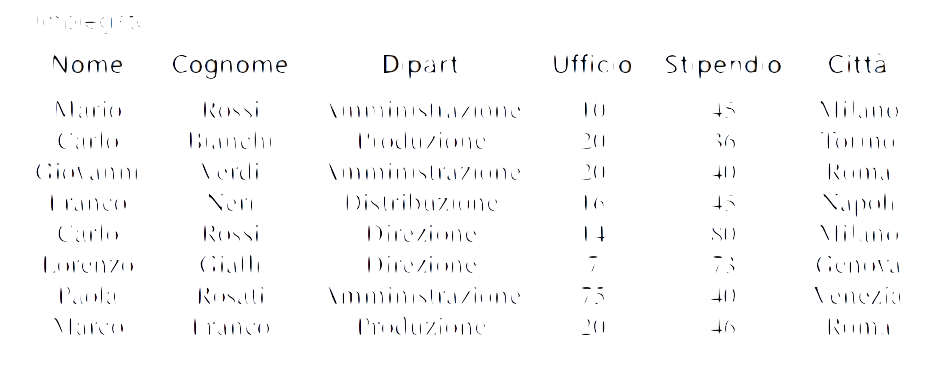
\includegraphics[width=0.5\textwidth]{images/tabella-impiegato.png}
      \end{center}

      \textbf{Estrarre lo stipendio degli impiegati di cognome ’Rossi’}
      \begin{sqlcode}
        SELECT *
        FROM Impiegato
          WHERE Cognome = 'Rossi';
      \end{sqlcode}

      Il risultato dell'interrogazione è la seguente tabella:

      \begin{center}
        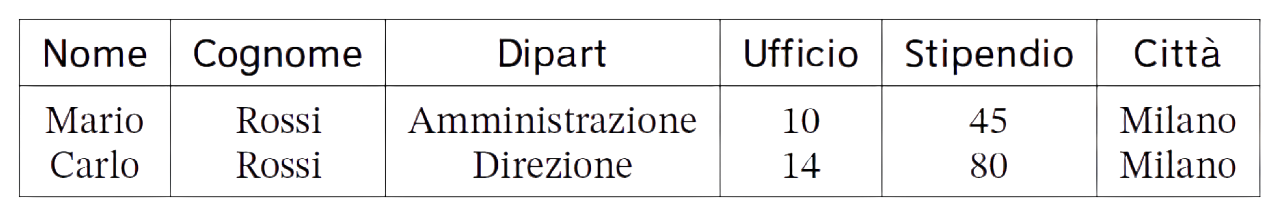
\includegraphics[width=0.6\textwidth]{images/select-all-impiegato.png}
      \end{center}
    \end{esempiobox}

    \bigskip
    L'attributo $\verb|AS|$ permette di rinominare un attributo (alias)
    \begin{sqlcode}
      SELECT nomeColonna AS nuovoNomeColonna
      FROM tabella;
    \end{sqlcode}

    \begin{esempiobox}{Interrogazione con \texttt{SELECT} usando \texttt{AS}}
      Consideriamo la seguente tabella:
      \begin{center}
        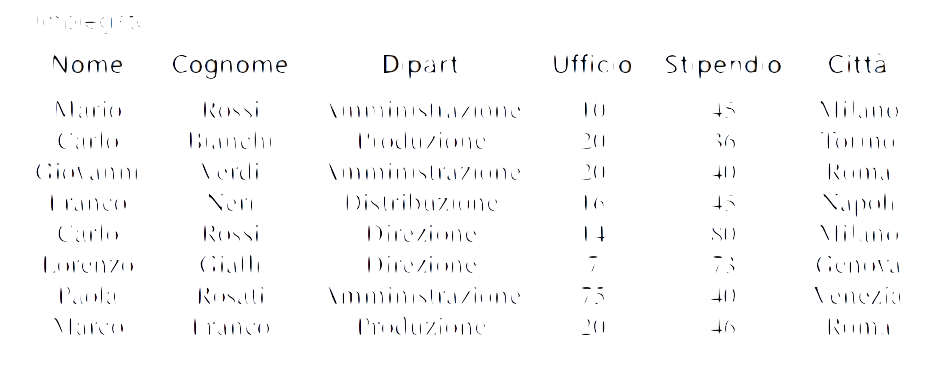
\includegraphics[width=0.5\textwidth]{images/tabella-impiegato.png}
      \end{center}

      \textbf{Estrarre lo stipendio degli impiegati di cognome ’Rossi’}
      \begin{sqlcode}
        SELECT Stipendio AS Salario
        FROM Impiegato
          WHERE Cognome = 'Rossi';
      \end{sqlcode}

      Il risultato dell'interrogazione è la seguente tabella:
      \begin{center}
        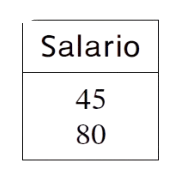
\includegraphics[width=0.2\textwidth]{images/select-alias-impiegato.png}
      \end{center}
    \end{esempiobox}


    \section{Clasuola \protect\texttt{FROM}}
    La clausola $\verb|FROM|$ specifica le tabelle da cui estrarre i dati.

    La sintassi dell'istruzione $\verb|FROM|$ è:
    \begin{sqlcode}
      FROM from_item [, ...]
    \end{sqlcode}

    dove $\verb|from_item|$ può essere una delle seguenti clausole:
    \begin{itemize}[label=$\triangleright$, itemsep=\medskipamount]
      \item \textbf{table\_name [[AS] alias [(column\_alias [, ...])]}: se sono presenti due o più tabelle, si esegue il prodotto cartesiano tra tutte le tabelle. 
      
      Se ci sono attributi con lo stesso nome su tabelle diverse, nella $\verb|SELECT|$ questi attributi sono identificati anteponendo il nome della tabella e un ’.’ (es. $\verb|nomeTabella.nomeAttributo|$)
      \item \textbf{(other\_select) [AS] nomeRisultato [(column\_alias [,...])]}: è una $\verb|SELECT|$ innestata. 
      
      Il risultato della $\verb|SELECT|$ interna è lo schema con nome $\verb|nomeRisultato|$ su cui fare la $\verb|SELECT|$ corrente.
      \item \textbf{from\_item [NATURAL] join\_type from\_item [ON condition]}: è la clausola JOIN. 
      
      Metodo più sofisticato di 1, che permette di selezionare un sottoinsieme del prodotto cartesiano di due o più tabelle. 
      
      $\verb|join_type|$ specifica il tipo di join
    \end{itemize}

    \begin{esempiobox}{Interrogazione con FROM}
      Consideriamo le seguenti tabelle:

      \begin{center}
        \begin{minipage}{0.45\textwidth}
          \centering
          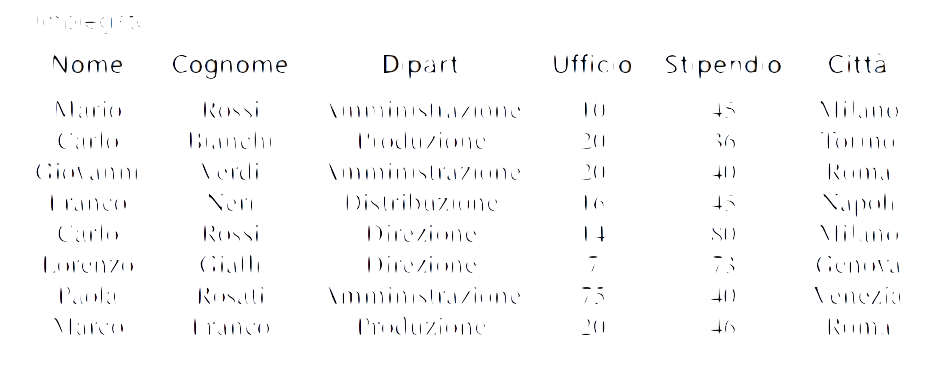
\includegraphics[width=\textwidth]{images/tabella-impiegato.png}
        \end{minipage}
        \hfill
        \begin{minipage}{0.45\textwidth}
          \centering
          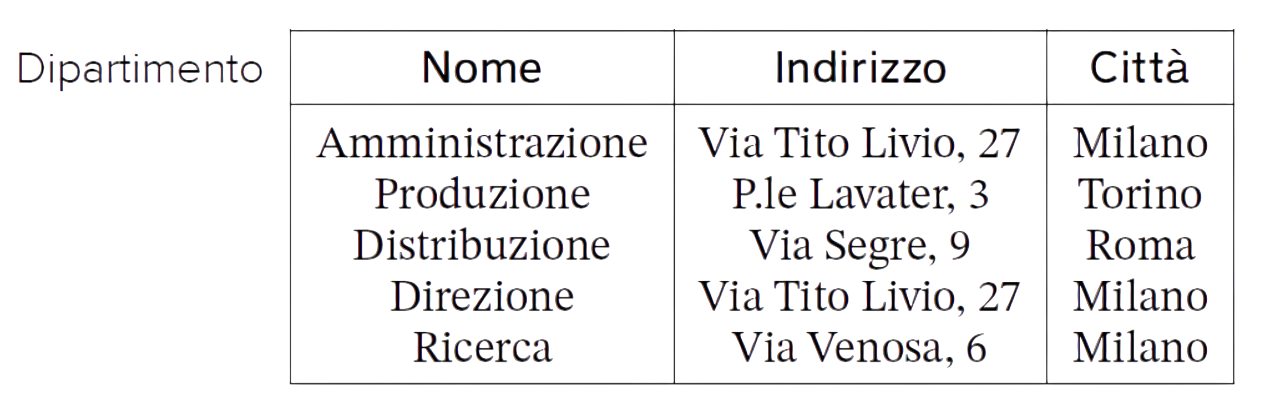
\includegraphics[width=\textwidth]{images/tabella-dipartimento.png}
        \end{minipage}
      \end{center}

      \textbf{Estrarre i nomi e il cognome degli impiegati e le città in cui lavorano}

      \begin{sqlcode}
        SELECT Impiegato.Nome, Impiegato.Cognome, 
               Dipartimento.Città
        FROM Impiegato, Dipartimento
          WHERE Impiegato.Dipart = Dipartimento.Nome
      \end{sqlcode}

      Il risultato dell'interrogazione è la seguente tabella:
      \begin{center}
        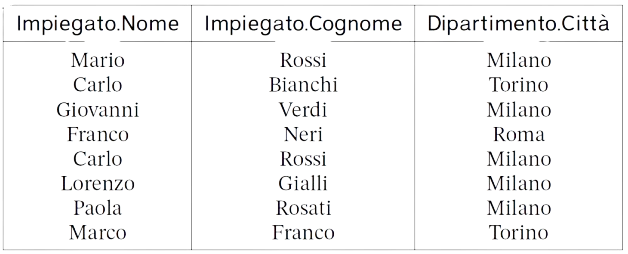
\includegraphics[width=0.4\textwidth]{images/from-impiegato-dipartimento.png}
      \end{center}
    \end{esempiobox}

    \section{Clausola WHERE}

    \begin{sqlcode}
      WHERE condition
    \end{sqlcode}

    La clausola $\verb|WHERE|$ ammette come argomento un’espressione booleana costruita combinando predicati semplici con gli operatori $\verb|AND|$, $\verb|OR|$ e $\verb|NOT|$:
    \begin{itemize}[label=$\circ$, itemsep=\smallskipamount]
      \item \textbf{AND}: seleziona le righe in cui tutti i predicati sono veri
      \item \textbf{OR}: seleziona le righe in cui almeno un predicato è vero
      \item \textbf{NOT}: seleziona le righe in cui il predicato è falso
    \end{itemize}
    
    Ciascun predicato semplice usa gli operatori $\verb|=|$, $\verb|<>| (\verb|<>| \Leftrightarrow \neq)$, $\verb|<|$, $\verb|>|$, $\verb|<=|$, $\verb|>=|$ per confrontare un’espressione costruita a partire dal valore di un attributo con un valore costante, oppure un’altra espressione.

    \begin{esempiobox}{Interrogazione con \texttt{WHERE}}
      Consideriamo le seguenti tabelle:
      \begin{center}
        \begin{minipage}{0.45\textwidth}
          \centering
          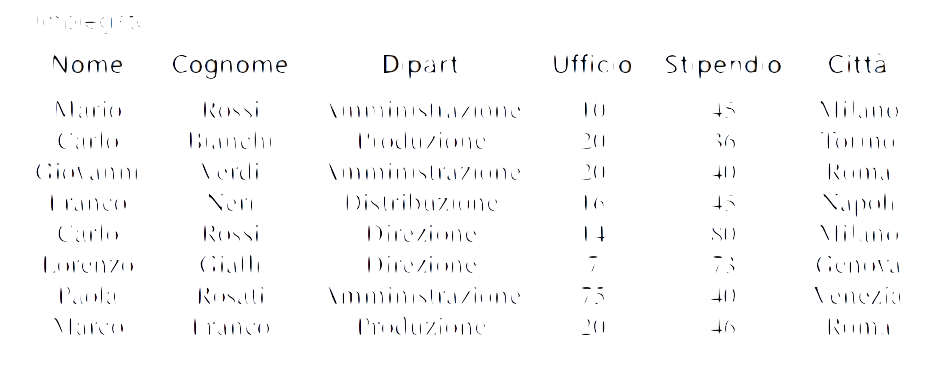
\includegraphics[width=\textwidth]{images/tabella-impiegato.png}
        \end{minipage}
        \hfill
        \begin{minipage}{0.45\textwidth}
          \centering
          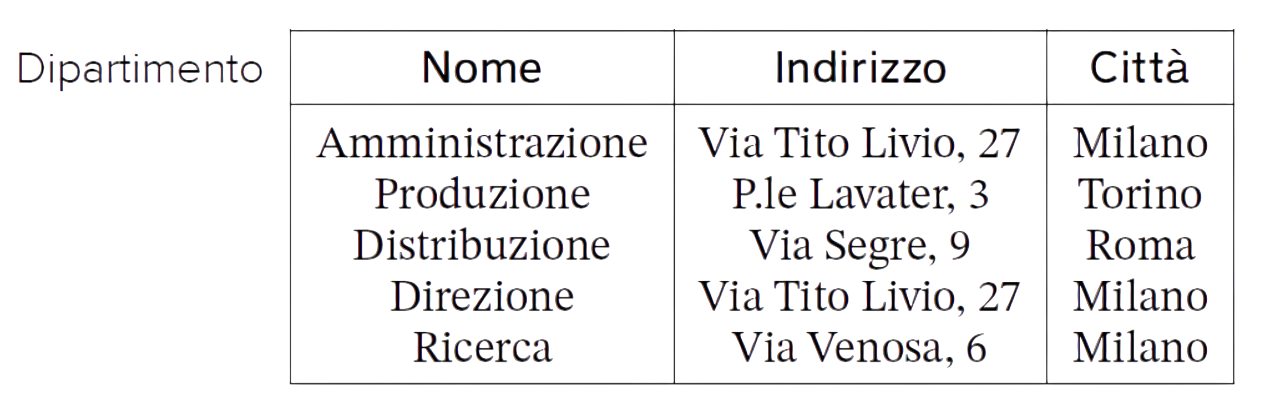
\includegraphics[width=\textwidth]{images/tabella-dipartimento.png}
        \end{minipage}
      \end{center}

      \textbf{Estrarre i nomi e il cognome degli impiegati che lavorano nell'ufficio 20 del dipartimento Ammistrazione}
      \begin{sqlcode}
        SELECT Nome, Cognome
        FROM Impiegato
          WHERE Ufficio = 20 AND Dipart = 'Amministrazione';
      \end{sqlcode}

      Il risultato dell'interrrogazione è la seguente tabella:
      \begin{center}
        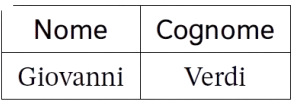
\includegraphics[width=0.3\textwidth]{images/where-impiegato-dipartimento.png}
      \end{center}
    \end{esempiobox}

    \subsection{Operatore \texttt{LIKE}}
    Per il confronto tra stringhe, SQL mette a disposizione anche l’operatore $\verb|LIKE|$ che consente di verificare se una stringa rispetta un certo “pattern” (oppure $\verb|ILIKE|$ per \textbf{case insentive}).

    I caratteri speciali per il confronto sono:
    \begin{itemize}[label=$\diamond$, itemsep=\smallskipamount]
      \item \textbf{\_}: confronto con un carattere arbitrario
      \item \textbf{\%}: confronto con una stringa di lunghezza arbitraria (anche 0) di caratteri arbitrari
    \end{itemize}

    \begin{esempiobox}{Interrogazione con LIKE}
      Consideriamo le seguenti tabelle:
      \begin{center}
        \begin{minipage}{0.45\textwidth}
          \centering
          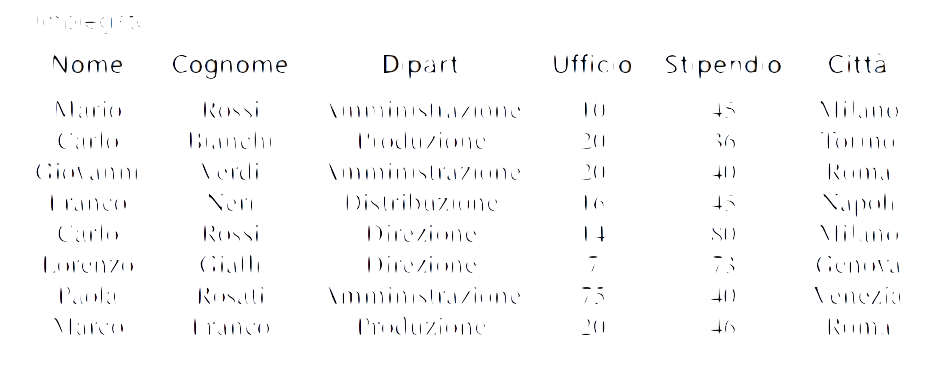
\includegraphics[width=\textwidth]{images/tabella-impiegato.png}
        \end{minipage}
        \hfill
        \begin{minipage}{0.45\textwidth}
          \centering
          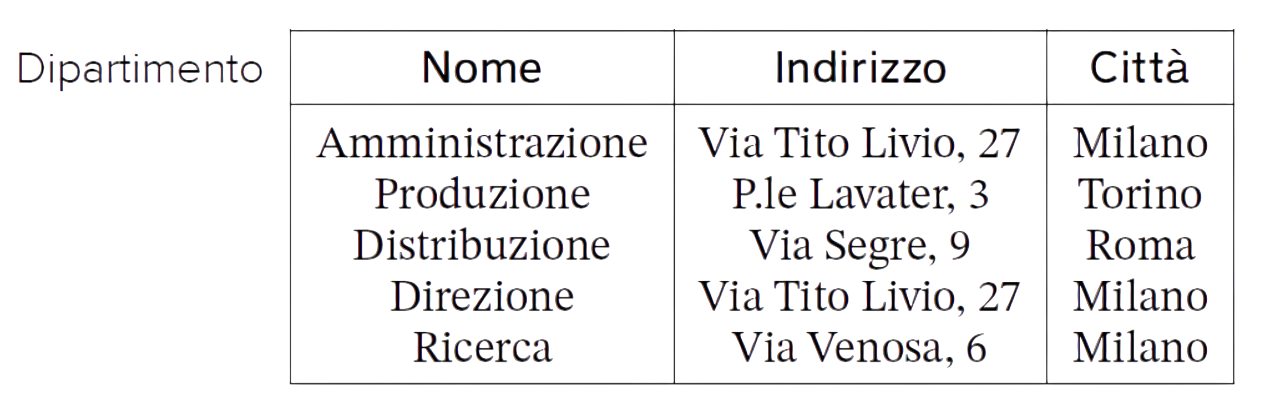
\includegraphics[width=\textwidth]{images/tabella-dipartimento.png}
        \end{minipage}
      \end{center}

      \textbf{Estrarre gli impiegati che hanno un cognome che ha una "o" in seconda posizione e finisce con una "i"}
      \begin{sqlcode}
       SELECT *
       FROM Impiegato
        WHERE Cogmome LIKE '_O%i'; 
      \end{sqlcode}

      Il risultato dell'interrogazione è la seguente tabella:
      \begin{center}
        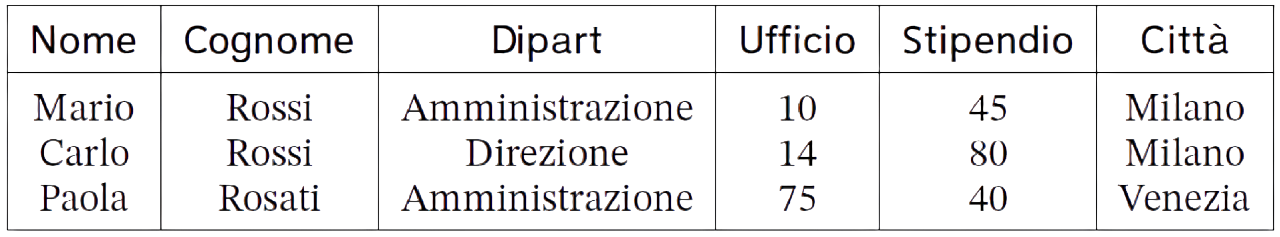
\includegraphics[width=0.4\textwidth]{images/like-impiegato-dipartimento.png}
      \end{center}
    \end{esempiobox}

    \subsection{Operatore \texttt{SIMILAR TO}}
    L’operatore $\verb|SIMILAR TO|$ è un $\verb|LIKE|$ più espressivo che accetta, come pattern, un sottoinsieme delle espressioni regolari POSIX (versione SQL).

    La sintassi delle espressioni regolari è:
    \begin{itemize}[label=$\circ$, itemsep=\smallskipamount]
      \item \textbf{\_}: un carattere qualsiasi
      \item \textbf{\%}: 0 o più caratteri qualsiasi
      \item \textbf{*}: ripetizione del precedente match 0 o più volte.
      \item \textbf{+}: ripetizione del precedente match UNA o più volte
      \item \textbf{{n,m}}: ripetizione del precedente match almeno n e non più di m volte
      \item \textbf{[...]}: ... è un elenco di caratteri ammissibili
    \end{itemize}

    \begin{esempiobox}{Interrogazione con \texttt{SIMILAR TO}}
      Consideriamo la seguente tabella:
      \begin{center}
        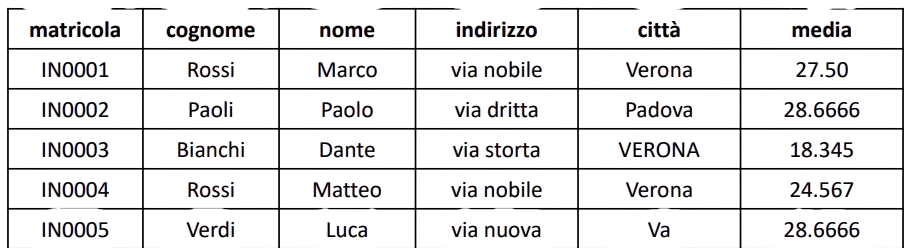
\includegraphics[width=0.5\textwidth]{images/studenti-tabella.png}
      \end{center}

      \textbf{Estrarre gli studenti con cognome che inizia con 'A' o 'B', o 'D', o 'N' e finisce con 'a}
      \begin{sqlcode}
        SELECT cognome, nome, città
        FROM Studente
          WHERE cognome SIMILAR TO '[ABDN]{1}%a';
      \end{sqlcode}

      Il risultato dell'interrogazione è la seguente tabella:
      \begin{center}
        
\includegraphics[width=0.4\textwidth]{images/similarTo-studenti.png}
      \end{center}
    \end{esempiobox}

    \subsection{Operatore \texttt{BETWEEN}}
    L’operatore BETWEEN consente di verificare se un valore è compreso tra due valori estremi (inclusi). 

    La sintassi è la seguente:
    \begin{sqlcode}
      condition BETWEEN value1 AND value2  
    \end{sqlcode}

    \begin{esempiobox}{Interrogazione con \texttt{BETWEEN}}
      Consideriamo la seguente tabella:
      \begin{center}
        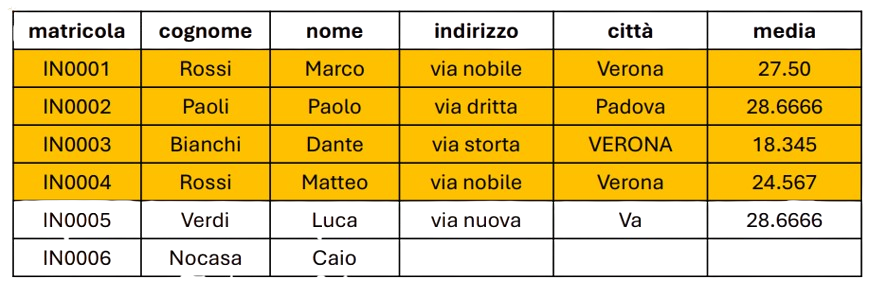
\includegraphics[width=0.5\textwidth]{images/studente-tabella.png}
      \end{center}

      \textbf{Estrarre tutti gli studenti che hanno matricola tra 'IN0002' e 'IN0004'}
      \begin{sqlcode}
        SELECT cognome, nome, città
        FROM Studente
          WHERE matricola BETWEEN 'IN0002' AND 'IN0004';  
      \end{sqlcode}

      Il risultato dell'interrogazione è:
      \begin{center}
        
\includegraphics[width=0.4\textwidth]{images/between-studente.png}
      \end{center}
    \end{esempiobox}


    \subsection{Operatore \texttt{IN}}
    Nella clausola $\verb|WHERE|$ può apparire l’operatore $\verb|[NOT] IN|$ per testare l’appartenenza di un valore ad un insieme. 
    
    La sintassi è la seguente:
    \begin{sqlcode}
      WHERE attributo [NOT] IN (valore, [, ...]);
    \end{sqlcode}

    \begin{esempiobox}{Interrogazione con \texttt{IN}}
      Consideriamo la seguente tabella:
      \begin{center}
        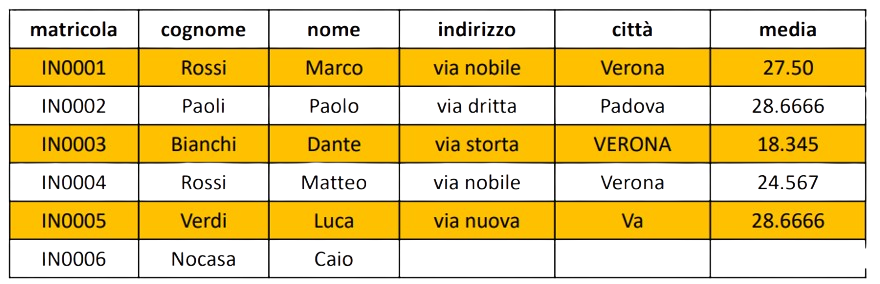
\includegraphics[width=0.5\textwidth]{images/studente-in-tabella.png}
      \end{center}

      \textbf{Estrarre tutti gli studenti che hanno matricola nell'elenco 'IN0001', 'IN0003' e 'IN0005'}
      \begin{sqlcode}
        SELECT cognome, nome, matricola
        FROM Studente
          WHERE matricola IN ('IN0001', 'IN0003', 'IN0005');  
      \end{sqlcode}

      Il risultato dell'interrogazione sono le righe gialle.
    \end{esempiobox}


    \subsection{Operatore \texttt{IS NULL}}
    Per verificare se un attributo ha un valore nullo o meno si utilizza il predicato $\verb|IS NULL|$ che ritorna true se l’attributo ha valore nullo (oppure $\verb|IS NOT NULL|$):
    \begin{itemize}[label=$\triangleright$, itemsep=\smallskipamount]
      \item \textbf{IS NULL}: ritorna true se l’attributo ha valore nullo
      \item \textbf{IS NULL}: è la negazione, ritorna true se l’attributo ha valore diverso da nullo
    \end{itemize}

    \begin{sqlcode}
      WHERE attributo IS [NOT] IN NULL;
    \end{sqlcode}

    SQL-2 implementa la logica a 3 valori:
    \begin{itemize}[itemsep=\smallskipamount]
      \item predicato semplice restituisce il valore $\verb|NULL|$ quando uno qualsiasi dei termini del predicato ha valore nullo
      \item predicato $\verb|IS NULL|$ è una eccezione, restituendo sempre il valore vero oppure false, mai il valore $\verb|NULL|$
    \end{itemize}

    \begin{esempiobox}{Interrogazione con \texttt{IS NULL}}
      Consideriamo la seguente tabella:
      \begin{center}
        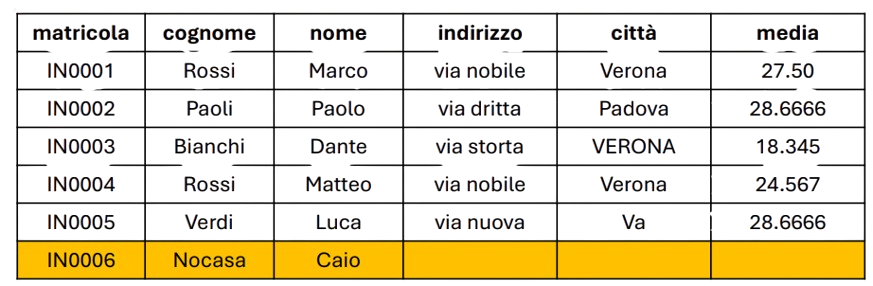
\includegraphics[width=0.5\textwidth]{images/studente-isNull-tabella.png}
      \end{center}

      \textbf{Estrarre tutti gli studenti che hanno matricola nell'elenco 'IN0001', 'IN0003' e 'IN0005'}
      \begin{sqlcode}
        SELECT cognome, nome, città
        FROM Studente
          WHERE città IS NULL;  
      \end{sqlcode}

      Il risultato dell'interrogazione sono le righe gialle.
    \end{esempiobox}



    \section{Gestione dei duplicati in SQL}
    Siccome la rimozione delle righe duplicate è un’operazione costosa, SQL le mantiene di default. 
    
    Per togliere i duplicati si può utilizzare la parola chiave $\verb|DISTINCT|$ dopo $\verb|SELECT|$:
    \begin{sqlcode}
      SELECT DISTINCT colonna
      FROM tabella
        WHERE condizione;
    \end{sqlcode}

    \begin{esempiobox}
      Consideriamo la seguente tabella:
      \begin{center}
        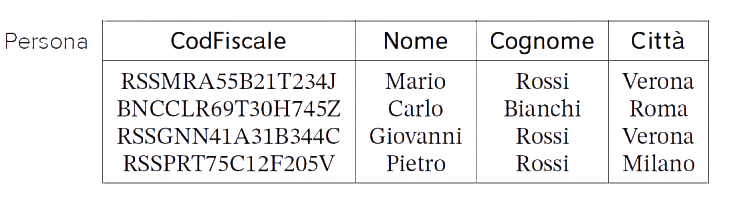
\includegraphics[width=0.5\textwidth]{images/persona-tabella.png}
      \end{center}

      \textbf{Estrarre le città delle persone in cui il cognome è Rossi}.

      \begin{sqlcode}
        SELECT Città
        FROM Persona
          WHERE Cognome = 'Rossi';
      \end{sqlcode}

      L'output di questa interrogazione è la tabella:
      \begin{center}
        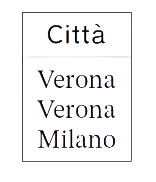
\includegraphics[width=0.3\textwidth]{images/persona-output.png}
      \end{center}

      Per togliere i duplicati si può utilizzare la parola chiave $\verb|DISTINCT|$ dopo $\verb|SELECT|$:
      \begin{sqlcode}
        SELECT DISTINCT Città
        FROM Persona
          WHERE Cognome = 'Città';
      \end{sqlcode}
      %foto
    \end{esempiobox}

    \section{Clausola \texttt{JOIN}}
    In SQL, le interrogazioni con la clausola \verb|JOIN| si possono definire in due modi:
    \begin{itemize}[label=$\triangleright$, itemsep=\smallskipamount]
      \item \textbf{senza l’uso di nuova sintassi}: specifica il legame tra le tabelle coinvolte a livello della clausola $\verb|WHERE|$
      \item \textbf{con l'uso di sintassi riservata} a livello di clausola $\verb|FROM|$
    \end{itemize}

    \smallskip
    La clausola \verb|FROM| ammette come argomento:
    \begin{sqlcode}
      tabella [[AS] name] [, ...]
    \end{sqlcode}

    Si è visto che se sono presenti due o più nomi di tabelle, si esegue il prodotto cartesiano tra tutte le tabelle e lo schema del risultato
    può contenere tutti gli attributi del prodotto cartesiano.\\[0.2ex]
    Il prodotto cartesiano di due o più tabelle è un $\verb|CROSS JOIN|$.

    \medskip
    A partire da SQL-2, esistono altri tipi di \texttt{JOIN}:
    \begin{itemize}[label=$\circ$, itemsep=\medskipamount]
      \item $\verb|INNER JOIN|$: restituisce solo le righe che soddisfano la condizione di join
      \item $\verb|LEFT [OUTER] JOIN|$: restituisce
      \begin{itemize}[label=$\diamond$, itemsep=\smallskipamount]
        \item tutte le righe della tabella di destra e sinistra che soddisfano la condizione di $\verb|join|$
        \item $\verb|null|$ per le righe della tabella di destra che non soddifisfano la condizione di di $\verb|join|$
      \end{itemize}
      \item $\verb|RIGH [OUTER] JOIN|$: restituisce
      \begin{itemize}[label=$\diamond$, itemsep=\smallskipamount]
        \item tutte le righe della tabella di destra e sinistra che soddisfano la condizione di $\verb|join|$
        \item $\verb|null|$ per le righe della tabella di sinistra che non soddifisfano la condizione di di $\verb|join|$
      \end{itemize}
      \item $\verb|FULL [OUTER] JOIN|$: restituisce
      \begin{itemize}[label=$\diamond$, itemsep=\smallskipamount]
        \item tutte le righe di entrambe le tabelle
        \item $\verb|null|$ per le righe che non soddifisfano la condizione di di $\verb|join|$
      \end{itemize}
    \end{itemize}

    In generale, la sintassi è:
    \begin{sqlcode}
      tabella [NATURAL] join_type table_name [ ON condition [, ...]]
    \end{sqlcode}

    \begin{itemize}[label=$\triangleright$]
      \item $\verb|condition|$: espressione booleana che seleziona le tuple del $\verb|join|$ da aggiungere al risultato
    \end{itemize}

    Le tuple selezionate possono essere poi filtrate con la condizione della clausola $\verb|WHERE|$.

    \begin{figure}[H]
      \centering
      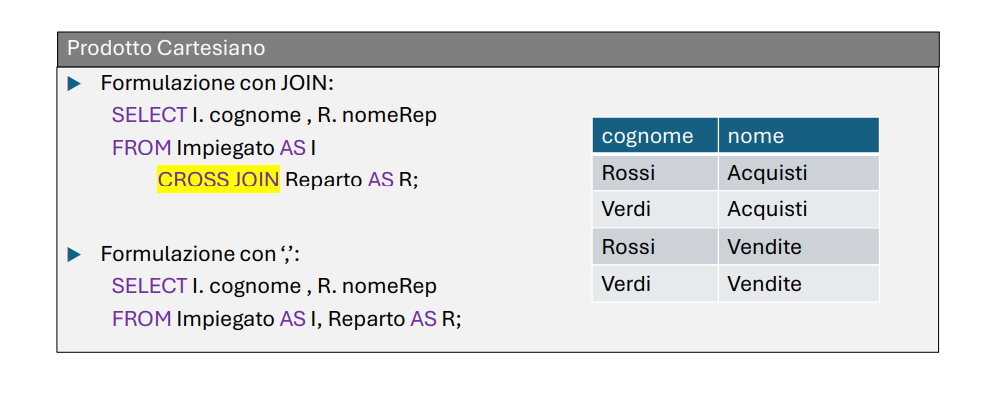
\includegraphics[width=\textwidth]{images/Join.png}
    \end{figure}

    \subsection{Clausola \texttt{INNER JOIN}}
    La sintassi è:
    \begin{sqlcode}
      tabella [ INNER ] JOIN tabella ON join_condition [, ...]
    \end{sqlcode}
    
    Rappresenta il tradizionale $\theta$ $\verb|join|$ dell’algebra relazionale.\\[0.2ex]
    Combina ciascuna riga $\mathrm{r_1}$ di $\mathrm{table_1}$ con ciascuna riga di $\mathrm{table_2}$ che soddisfa la condizione della clausola $\verb|ON|$.

    \begin{esempiobox}{Interrogazione con \texttt{INNER JOIN}}
      \begin{sqlcode}
        SELECT I.cognome, R.nomeRep, R.sede
        FROM Impiegato AS I
        INNER JOIN Reparto AS R ON I.nomeRep = R.nomeRep;
      \end{sqlcode}

      \begin{center}
        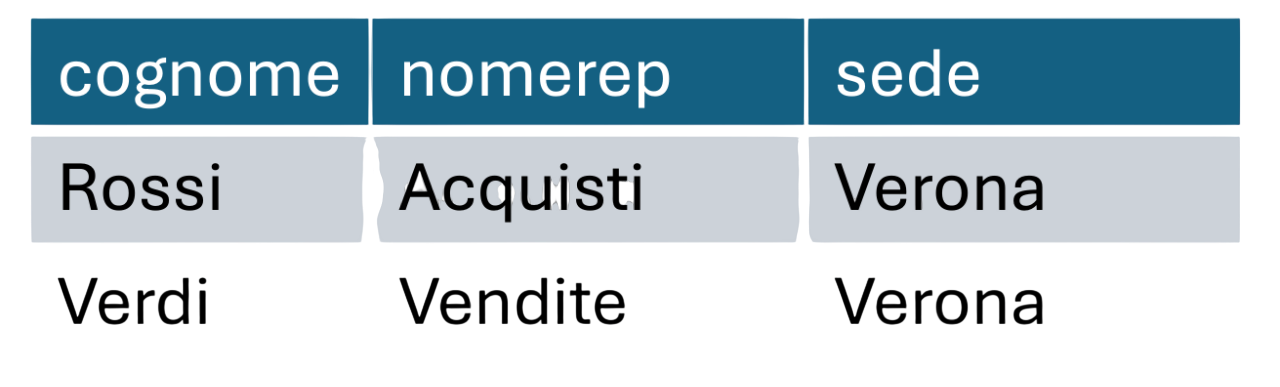
\includegraphics[width=0.5\textwidth]{images/tabellina.png}
      \end{center}
    \end{esempiobox}
    
    \subsection{Clausola \texttt{LEFT OUTER JOIN}}
    La sintassi è:
    \begin{sqlcode}
      tabella LEFT [ OUTER ] JOIN tabella ON join_condition [, ...]
    \end{sqlcode}

    Si esegue un $\verb|INNER JOIN|$.\\[0.2ex]
    Poi, per ciascuna riga r1 di table1 che non soddisfa la condizione con qualsiasi riga di $\mathrm{table_2}$, si aggiunge una riga al risultato con i valori di $\mathrm{r_1}$ e assegnando $\verb|NULL|$ agli altri attributi.

    \begin{esempiobox}{Interrogazione con \texttt{LEFT [OUTER] JOIN}}
      \begin{sqlcode}
        INSERT INTO Reparto (nomerep, sede, telefono)
        VALUES ('Finanza', 'Padova', '02 8028888');

        SELECT R.nomeRep, I.cognome
        FROM Reparto AS R
        LEFT OUTER JOIN Impiegato AS I ON I.nomerep = R.nomerep;
      \end{sqlcode}

      \begin{center}
        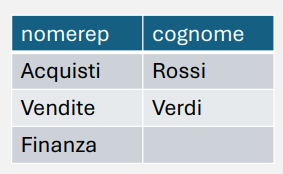
\includegraphics[width=0.4\textwidth]{images/tabellina2.png}
      \end{center}
    \end{esempiobox}

    \vario{Nota}{
      Il $\texttt{LEFT OUTER JOIN}$ non è simmetrico!

      \smallskip
      Con le medisime tabelle si possono ottenere risultati diversi invertendo l’ordine delle tabelle nel join!
    }
    
    \subsection{Clausola \texttt{RIGHT OUTER JOIN}}
    La sintassi è:
    \begin{sqlcode}
      tabella RIGHT [ OUTER ] JOIN tabella ON join_condition [, ...]
    \end{sqlcode}

    \begin{esempiobox}{Interrogazione con \texttt{RIGHT [OUTER] JOIN}}
      \begin{sqlcode}
        SELECT I.cognome , R.nomeRep
        FROM Impiegato I 
        RIGHT OUTER JOIN Reparto AS R ON I. nomerep = R. nomerep;
      \end{sqlcode}

      \begin{center}
        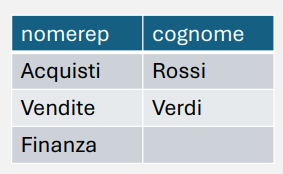
\includegraphics[width=0.5\textwidth]{images/tabellina2.png}
      \end{center}
    \end{esempiobox}
    
    \subsection{Clausola \texttt{FULL OUTER JOIN}}
    Ls sintassi è:
    \begin{sqlcode}
      tabella FULL [ OUTER ] JOIN tabella ON join_condition [, ...]
    \end{sqlcode}
    
    È equivalente a:
    \begin{sqlcode}
      INNER JOIN + LEFT OUTER JOIN + RIGHT OUTER JOIN
    \end{sqlcode}

    Non è equivalente a $\verb|CROSS JOIN|$.

    \section{Uso di variabili (alias)}
    SQL permette di associare un nome alternativo (alias) alle tabelle che compaiono nella clausola $\verb|FROM|$.\\[0.2ex]
    Il nome viene usato per far riferimento alla tabella nel contesto dell’interrogazione per diversi motivi:
    \begin{itemize}[label=$\triangleright$, itemsep=\smallskipamount]
      \item far riferimento alla tabella in modo compatto
      \item fare accesso più volte alla stessa tabella
    \end{itemize}

    \begin{esempiobox}{Interrogazione con utilizzo di \texttt{AS}}
      Consideriamo la seguente tabella:

      \begin{center}
        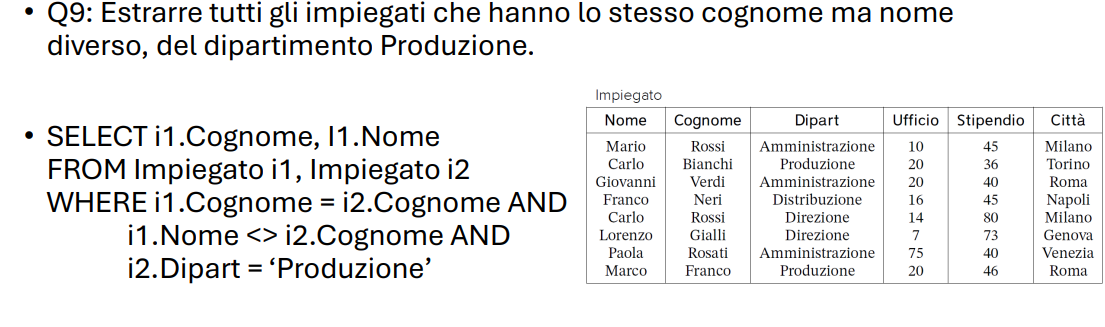
\includegraphics[width=0.6\textwidth]{images/Q9.png}
      \end{center}

      \textbf{Estrarre tutti gli impiegati che hanno lo stesso cognome, ma nome diverso del dipartimento Produzione}
      \begin{sqlcode}
        SELECT I1.Cognome, I2.Cognome
        FROM Impiegato I1, Impiegato I2
        WHERE I1.Cogmome = I2.Cognome AND
          I1.Nome <> I2.Cognome AND
          I2.Dipart = 'Produzione;
      \end{sqlcode}

      Questa interrogazione confronta ciascuna riga di Impiegato con tutte le righe di Impiegato associate al dipartimento Produzione.

      \smallskip
      Si può immaginare che al momento della definizione dell’alias vengano create due copie della tabella Impiegato, ciascuna associata ad una delle due variabili i1 e i2.

      \smallskip
      Le due copie contengono tutte le righe di Impiegato.

      \smallskip
      Sulla copia i2 vengono selezionate solo le righe del dipartimento `Produzione'.
      \begin{center}
         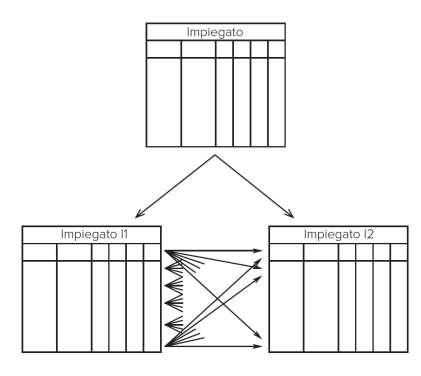
\includegraphics[width=0.5\textwidth]{images/Alias.png}
      \end{center}
    \end{esempiobox}
    
    \section{Clausola \texttt{ORDER BY}}
    Una relazione è un insieme di tuple non ordinato, però, sorge spesso il bisogno di costruire un ordine sulle righe.\\[0.2ex]
    SQL permette di specificare un ordinamento (ascendente o discendente) sulle righe dell‘output grazie alla clausola $\verb|ORDER BY|$ che chiude l‘interrogazione.

    La sintassi è:
    \begin{sqlcode}
      ORDER BY attributo [{ ASC | DESC }] [, ... ];
    \end{sqlcode}
    
    Le righe vengono ordinate per il primo attributo nell’elenco, a parità di valore del primo attributo si usa il secondo e così via in sequenza.

    Di default l'ordinamento è $\verb|ASC|$.

    \begin{esempiobox}{Interrogazione con \texttt{ORDER BY}}
      Consideriamo la seguente tabella:

      \begin{center}
        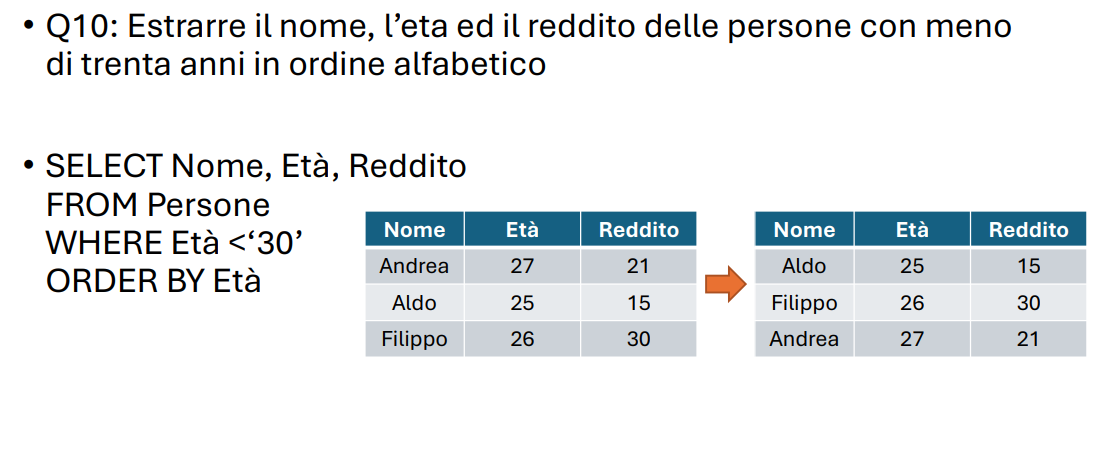
\includegraphics[width=0.5\textwidth]{images/Q10.png}
      \end{center}

      \textbf{Estrarre il nome, l'età e il reddito delle persone con meno di 30 anni in ordine alfabetico}.

      \begin{sqlcode}
        SELECT Nome, Età, Reddito
        FROM Persone
          WHERE Età < 30
            ORDER BY Età;
      \end{sqlcode}
    \end{esempiobox}

    \begin{esempiobox}{Interrogazione con \texttt{ORDER BY}}
      Consideriamo la seguente tabella:

      \begin{center}
        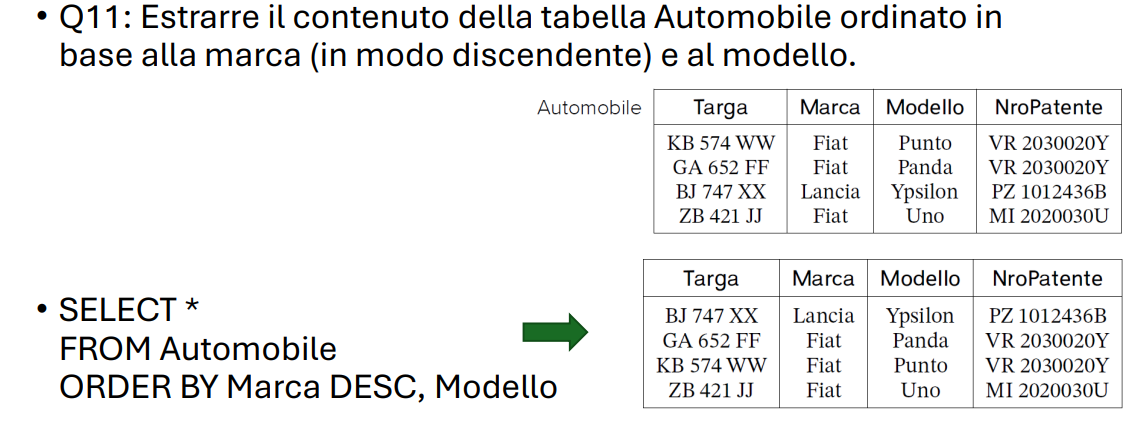
\includegraphics[width=0.5\textwidth]{images/Q11.png}
      \end{center}

      \textbf{Estrarre il contenuto della tabella Automobile ordinato in base alla marca (discendente) e al modello}.

      \begin{sqlcode}
        SELECT *
        FROM Automobile
          ORDER BY Marca DESC, Modello;
      \end{sqlcode}
    \end{esempiobox}

    \section{Operazioni insiemistiche}
    SQL mette a disposizione degli operatori insiemistci:
    \begin{sqlcode}
      SELECT
        { UNION | INTERSECT | EXCEPT 
        [ALL] SELECT }
    \end{sqlcode}
    
    Gli operatori insiemistici, al contrario del resto del linguaggio, assumono come default di eseguire un’eliminazione dei duplicati, a meno che si usi $\verb|ALL|$.\\[0.2ex]
    Sono sufficienti domini compatibili ed ugual numero di attributi.\\[0.2ex]
    La corrispondenza si basa sulla posizione e se i nomi degli attributi sono diversi di solito il sistema usa il nome del primo operando.

    \subsection{Unione}
    \begin{esempiobox}{Interrogazione con unione}
      Consideriamo la seguente tabella:

      \begin{center}
        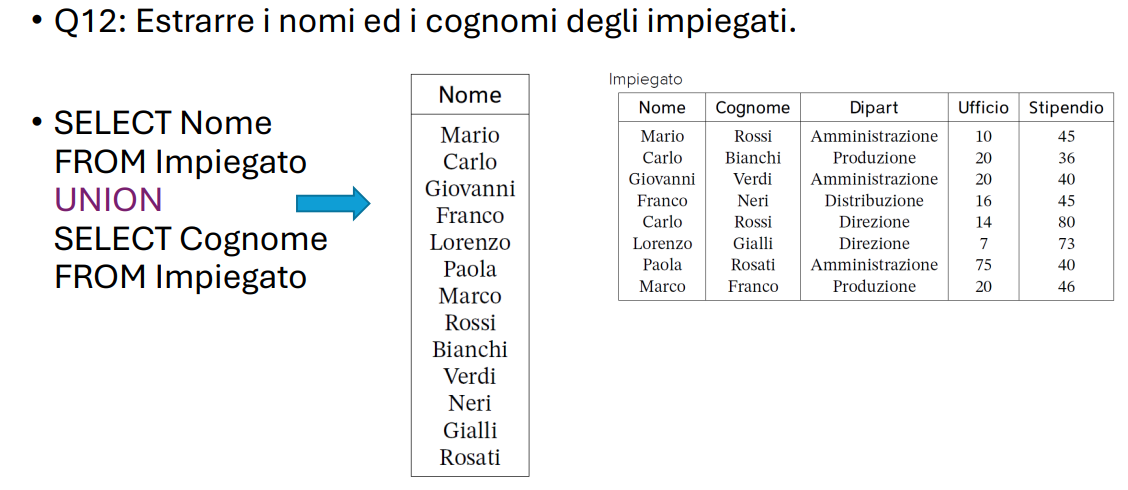
\includegraphics[width=0.5\textwidth]{images/Q12.png}
      \end{center}

      \textbf{Estrarre i nomi e i cognomi degli impiegati}.

      \begin{sqlcode}
        SELECT Nome
        FROM Impiegato
        UNION
        SELECT Cognome
        FROM Impiegato
      \end{sqlcode}
    \end{esempiobox}

    \begin{esempiobox}{Interrogazione con unione}
      Consideriamo la seguente tabella:

      \begin{center}
        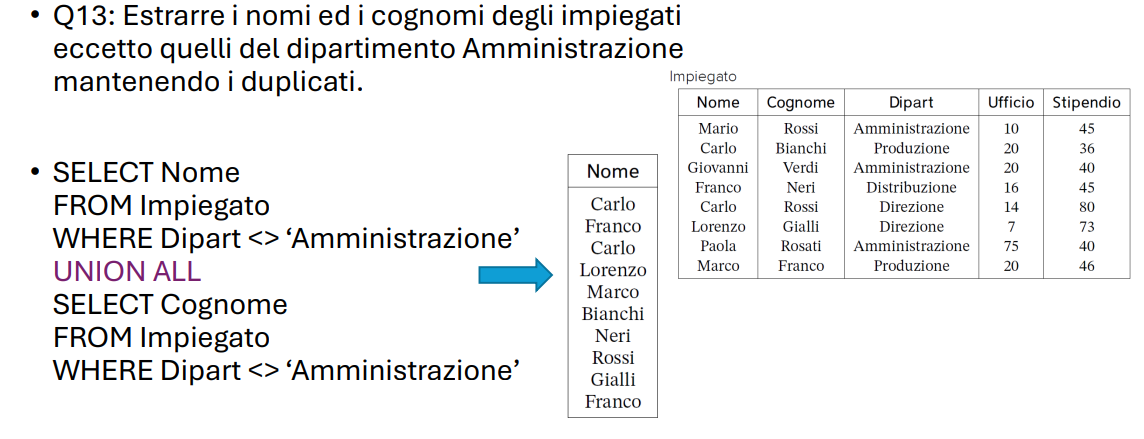
\includegraphics[width=0.5\textwidth]{images/Q13.png}
      \end{center}

      \textbf{Estrarre i nomi e i cognomi degli impiegati eccetto quelli del dipartimento Amministrazione mantenendo i duplicati}.

      \begin{sqlcode}
        SELECT Nome
        FROM Impiegato
          WHERE Diaprt <> 'Amministrazione'
        UNION ALL
        SELECT Cognome
        FROM Impiegato
          WHERE Diaprt <> 'Amministrazione';
      \end{sqlcode}
    \end{esempiobox}

    \subsection{Intersezione}
    \begin{esempiobox}{Interrogazione con intersezione}
      Consideriamo la seguente tabella:

      \begin{center}
        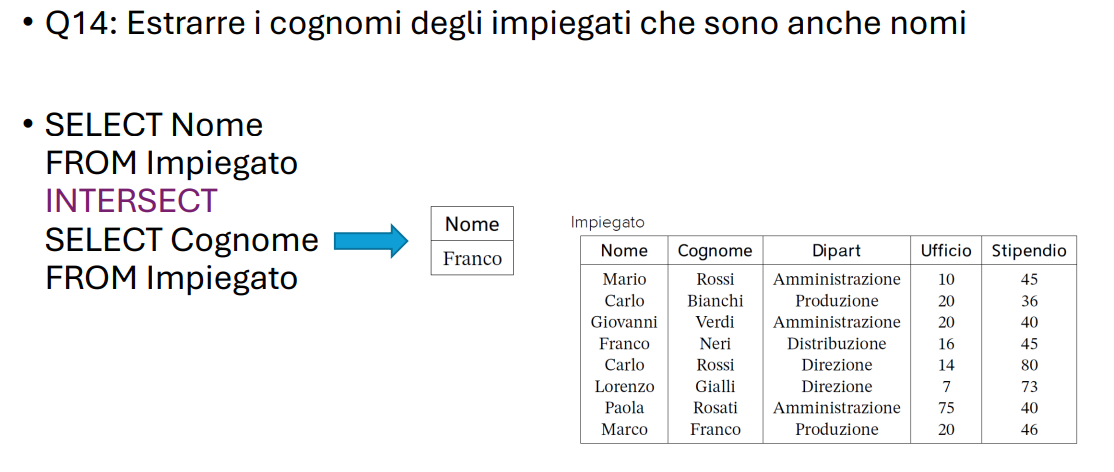
\includegraphics[width=0.5\textwidth]{images/Q14.png}
      \end{center}

      \textbf{Estrarre i cognomi degli impiegati che sono anche nomi}.

      \begin{sqlcode}
        SELECT Nome
        FROM Impiegato
        INTERSECT
        SELECT Cognome
        FROM Impiegato;
      \end{sqlcode}
    \end{esempiobox}

    \subsection{Differenza}
    \begin{esempiobox}{Interrogazione con differenza}
      Consideriamo la seguente tabella:

      \begin{center}
        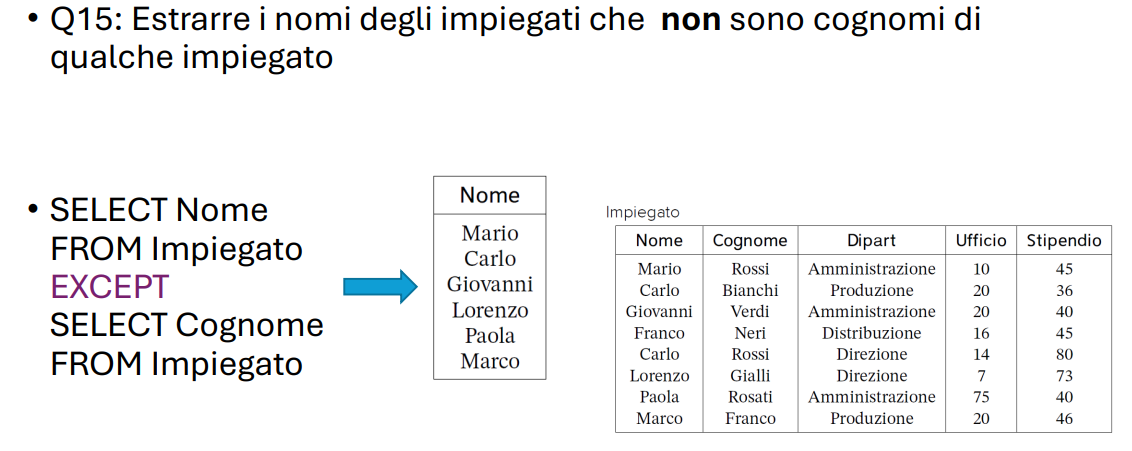
\includegraphics[width=0.5\textwidth]{images/Q15.png}
      \end{center}

      \textbf{Estrarre i nomi degli impiegati che non sono cognomi di qualche impiegato}.

      \begin{sqlcode}
        SELECT Nome
        FROM Impiegato
        EXCEPT
        SELECT Cognome
        FROM Impiegato;
      \end{sqlcode}
    \end{esempiobox}

    \section{Operatori aggregati}
    Gli operatori di aggregazione permettono di valutare proprietà che dipendono da insiemi di tuple.

    \subsection{Operatore \texttt{COUNT}}
    L'operatore $\verb|COUNT|$ conta il numero di righe di una tabella o il numero di valori di uno o più attributi.

    La sintassi è:
    \begin{sqlcode}
      COUNT ( < * | [DISTINCT | ALL] ListaAttributi > )
    \end{sqlcode}

    \begin{itemize}[label=$\triangleright$, itemsep=\smallskipamount]
        \item $\verb|*|$: conta il numero di righe della tabella
        \item $\verb|DISTINCT ListaAttributi|$: conta il numero di valori diversi degli attributi ListaAttributi
        \item $\verb|ALL ListaAttributi|$: conta il numero di righe che hanno valori diversi da NULL negli attributi in ListaAttributi (default)
    \end{itemize}

    \begin{esempiobox}{Interrogazione con \texttt{COUNT}}
      Consideriamo la seguente tabella:
      \begin{center}
        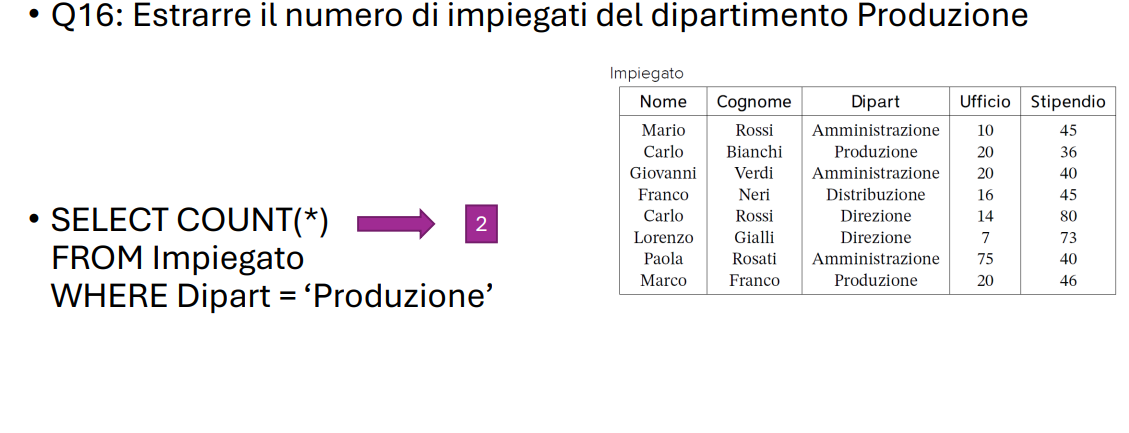
\includegraphics[width=0.5\textwidth]{images/Q16.png}
      \end{center}

      \textbf{Estrarre il numero di impiegati del dipartimento di Produzione}
      \begin{sqlcode}
        SELECT COUNT(*)
        FROM Impiegato
          WHERE Diaprt = 'Produzione';
      \end{sqlcode}
    \end{esempiobox}

    \begin{esempiobox}{Interrogazione con \texttt{COUNT}}
      Consideriamo la seguente tabella:
      \begin{center}
        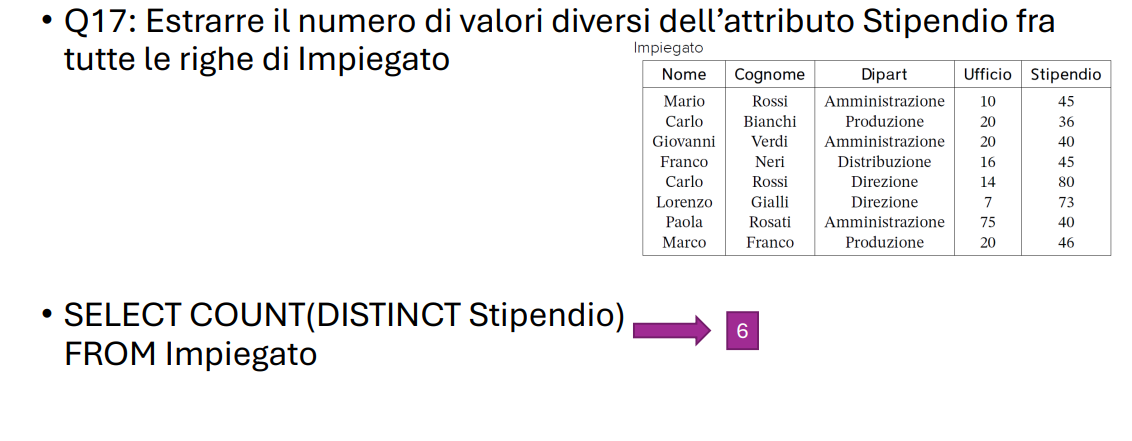
\includegraphics[width=0.5\textwidth]{images/Q17.png}
      \end{center}

      \textbf{Estrarre il numero di valori diversi dell'attributo Stipendio fra tutte le righe di Impiegato}
      \begin{sqlcode}
        SELECT COUNT(DISTINCT Stipendio)
        FROM Impiegato;
      \end{sqlcode}
    \end{esempiobox}

    \subsection{Operatore \texttt{SUM}}
    L'operatore $\verb|SUM|$ estituisce la somma dei valori posseduti dall’espressione.

    La sintassi è:
    \begin{sqlcode}
      SUM ( < * | [DISTINCT | ALL] ListaAttributi > )
    \end{sqlcode}

    \begin{esempiobox}{Interrogazione con \texttt{COUNT}}
      Consideriamo la seguente tabella:
      \begin{center}
        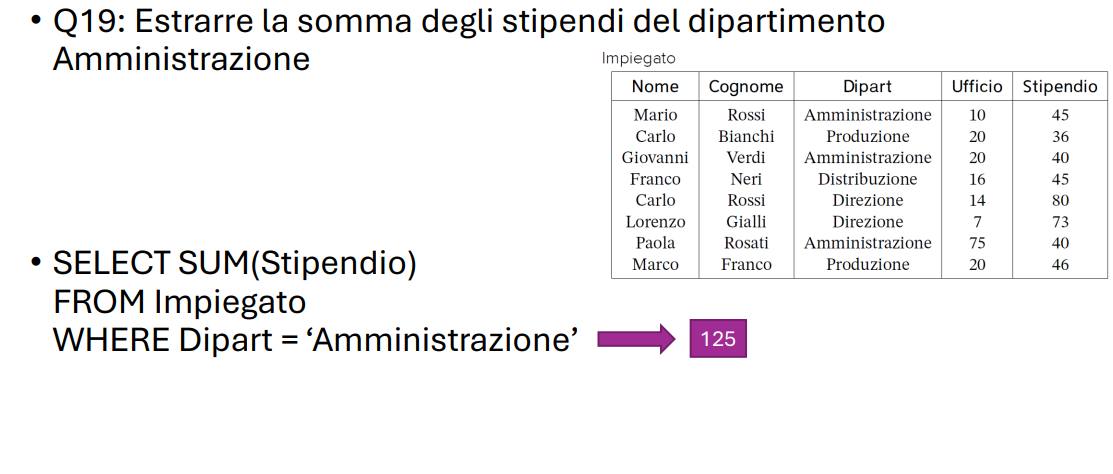
\includegraphics[width=0.5\textwidth]{images/Q19.png}
      \end{center}

      \textbf{Estrarre la somma degli stipendi del dipartimento Amministrazione}
      \begin{sqlcode}
        SELECT SUM(Stipendio)
        FROM Impiegato
          WHERE Dipart = 'Amministrazione';
      \end{sqlcode}
    \end{esempiobox}

    \subsection{Operatore \texttt{MAX/MIN}}
    Gli operatori $\verb|MIN|$ e $\verb|MAX|$ restituiscono rispettivamente il massimo e il minimo dei valori posseduti dall’espressione.

    La sintassi è:
    \begin{sqlcode}
      <MAX | MIN> ( [DISTINCT | ALL] ListaAttributi )
    \end{sqlcode}
    
    \subsection{Operatore \texttt{AVG}}
    L'operatore $\verb|AVG|$ restiusce la media dei valori.

    La sintassi:
    \begin{sqlcode}
      AVG ( [DISTINCT | ALL] ListaAttributi )
    \end{sqlcode}

    \begin{esempiobox}{Interrogazione con \texttt{MIN, MAX, AVG}}
      Consideriamo la seguente tabella:
      \begin{center}
        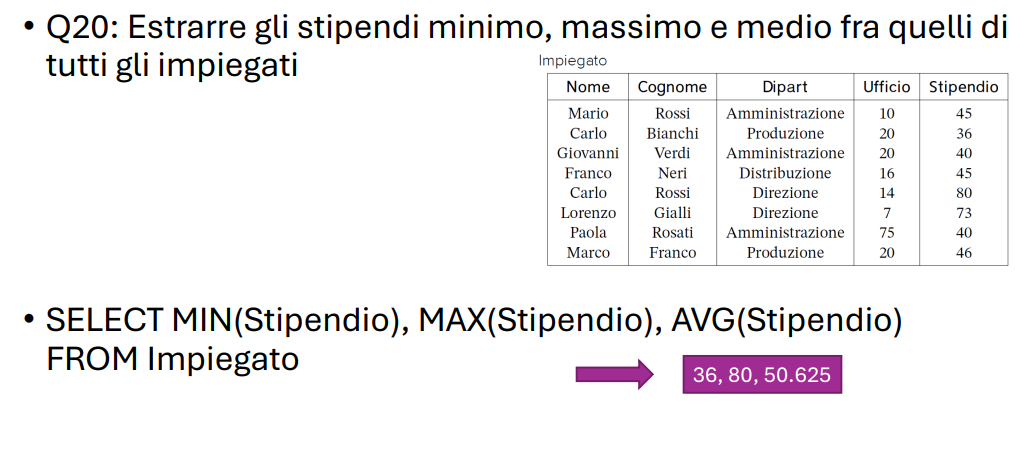
\includegraphics[width=0.5\textwidth]{images/Q20.png}
      \end{center}

      \textbf{Estrarre gli Stipendi minimi, massimi e medi fra quelli di tutti gli impiegati}
      \begin{sqlcode}
        SELECT MIN(Stipendio), MAX(Stipendio), AVG(Stipendio)
        FROM Impiegato;
      \end{sqlcode}
    \end{esempiobox}

    \vario{Nota}{
      \begin{itemize}[label=$\triangleright$, itemsep=\smallskipamount]
      \item $\texttt{SUM}$ e $\texttt{AVG}$ ammettono come argomento solo espressioni che rappresentano valori numerici o intervalli di tempo
      \item $\texttt{MAX}$ e $\texttt{MIN}$ ammettono come argomento solo espressioni su cui è definito un ordinamento (quindi anche stringhe)
      \item $\texttt{DISTINCT}$ elimina i duplicati
      \item $\texttt{ALL}$ trascura solo i valori nulli
    \end{itemize}
    }

    \begin{esempiobox}{ATTENZIONE}
      \begin{sqlcode}
        SELECT Cognone, Nome, MAX(I.Stipendio)
        FROM Impiegato AS I
        JOIN Diparmento AS D ON I.Dipart = D.Nome
          WHERE D.Città = 'Milano';
      \end{sqlcode}

      \textcolor{black!60!red}{\textbf{La seguente interrogazione non è corretta!}}
      
      \smallskip
      Gli operatori aggregati non sono un meccanismo di selezione, ma solo funzioni che restituiscono un valore quando sono applicate ad un insieme.
  
      \smallskip
      Cognome e Nome restituiscono un valore per ogni tupla selezionata, mentre $\texttt{MAX}$ restituisce un valore unico per tutto l’insieme.

      \smallskip
      Per risolvere questa situazione serve il meccanismo di \textbf{raggruppamento}.
    \end{esempiobox}


  \section{Clausola \texttt{GROUP BY}}
  Gli operatori aggregate possono essere applicati separatamente a sottoinsiemi di righe.\\[0.2ex]
  La clausola $\verb|GROUP BY|$ permette di specificare come dividere le tabelle in sottoinsiemi.\\[0.2ex]
  La clausola permette di specificare un insieme di attributi e l’interrogazione raggrupperà le righe che possiedono gli stessi valori per questo insieme di attributi.

  \begin{esempiobox}{Interrogazione con \texttt{GROUP BY}}
    Consideriamo la seguente tabella:
    \begin{center}
      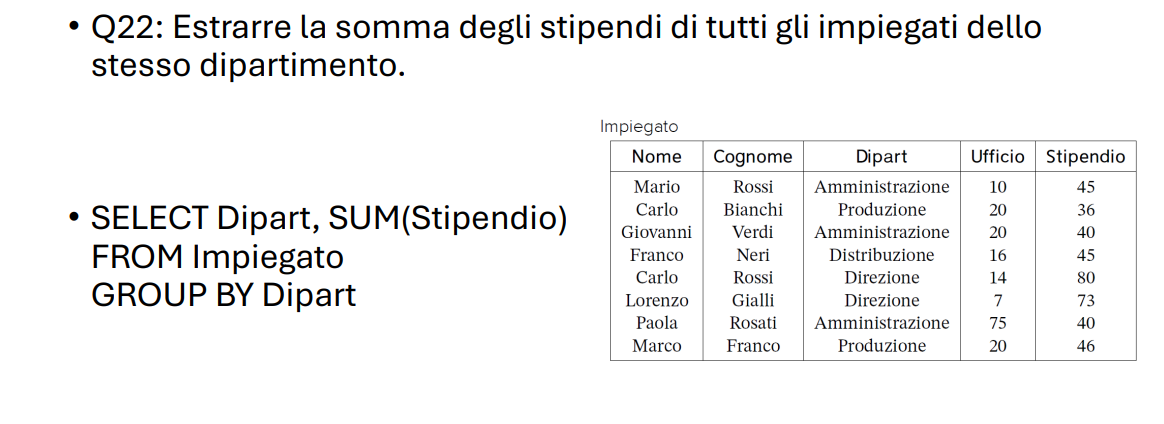
\includegraphics[width=0.5\textwidth]{images/Q22.png}
    \end{center}

    {\raggedright \textbf{Estrarre la somma degli stipendi di tutti gli impiegati dallo stesso dipartimento}\par}

    \begin{sqlcode}
      SELECT Dipart, SUM(Stipendio)
      FROM Impiegato
        GROUP BY Diaprt;
    \end{sqlcode}
  \end{esempiobox}

  In una interrogazione che fa uso della clausola $\verb|GROUP BY|$ può comparire come argomento della $\verb|SELECT|$ solo un sottoinsieme degli attributi usati nella clausola $\verb|GROUP BY|$, oppure, operatori di aggregazione.

  \subsection{Clausola \texttt{HAVING}}
  È possibile applicare delle selezioni ai gruppi generati tramite la clausola $\verb|GROUP BY|$.\\[0.2ex]
  La clausola $\verb|HAVING|$ permette di specificare delle condizioni che devono essere soddisfatte dai gruppi generati dopo l’esecuzione del raggruppamento tramite $\verb|GROUP BY|$.

  La sintassi è:
  \begin{sqlcode}
    SELECT Dipart, SUM(Stipendio) AS SommaStipendi
    FROM Impiegato
      GROUP BY Dipart
        HAVING SUM(Stipendio) > 100;
  \end{sqlcode}

  Dopo aver eseguito i raggruppamenti, vengono mantenuti solo i gruppi che soddisfano la condizione specificata nella clausola $\verb|HAVING|$.

  \begin{figure}[H]
    \centering
    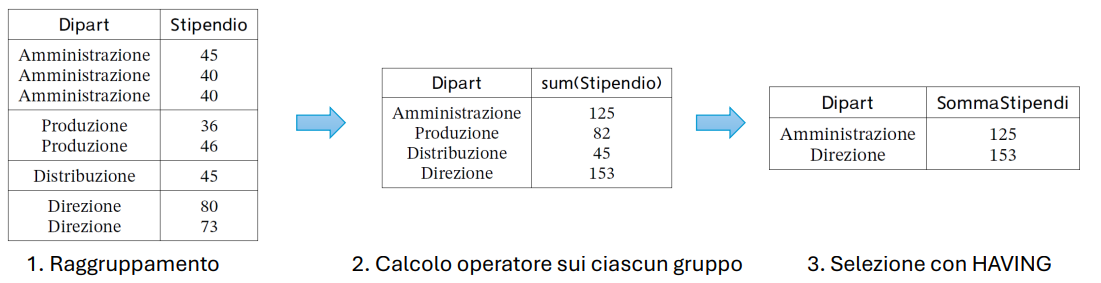
\includegraphics[width=\textwidth]{images/esempio.png}
  \end{figure}

  \begin{esempiobox}{OSSERVAZIONE}
    \begin{itemize}[label=$\triangleright$, itemsep=\smallskipamount]
      \item clausola $\texttt{WHERE}$ applica delle selezioni su singole righe, \textcolor{purple}{\textbf{prima}} dell’eventuale raggruppamento tramite $\texttt{GROUP BY}$
      \item clausola $\texttt{HAVING}$ applica delle selezioni su gruppi, generati a \textcolor{purple}{\textbf{seguito}} dell’esecuzione del raggruppamento tramite $\texttt{GROUP BY}$
    \end{itemize}

    \begin{sqlcode}
        SELECT Dipart
        FROM Impiegato
          WHERE Ufficio = 20 -- seleziona righe raggruppate
            GROUP BY Dipart  -- forma gruppi con righe selezionate
              HAVING AVG(Stipendio) > 25; -- seleziona gruppi del risultato
      \end{sqlcode}
  \end{esempiobox}

  \section{Interrogazioni nidificate}
  Un' interrogazione nidificata è un'interrogazione che contiene al suo interno altre interrogazioni.\\[0.2ex]
  La nidificazione può avvenire sia nella clausola $\verb|SELECT|$, che nella clausola $\verb|FROM|$, che nella clausola $\verb|WHERE|$.\\[0.2ex]
  Il caso tipico è la nidificazione nella clausola $\verb|WHERE|$, dove un predicato contiene un confronto tra un valore (espressione su una singola riga) ed il risultato di un’interrogazione SQL.

  \subsection{Clausola \texttt{WHERE}}
  Se in un predicato si confronta un attributo o una espressione che produce un valore singolo con il risultato di un’interrogazione, sorge il problema di disomogeneità dei termini del confronto.\\[0.2ex]
  I normali operatori di confronto ($\verb|=|, \verb|<>|, \verb|<|, \verb|>|, \verb|<=|, \verb|=>|$) possono essere estesi con le parole chiave $\verb|ANY|$ e $\verb|ALL|$:
  \begin{itemize}[label=$\triangleright$, itemsep=\smallskipamount]
    \item $\verb|ANY|$: riga soddisfa la condizione se risulta vero il confronto (con l’operatore specificato) tra il valore dell’attributo (o espressione) e \textbf{almeno} uno degli elementi restituiti dall’interrogazione 
    \item $\verb|ALL|$: riga soddisfa la condizione se risulta vero il confronto (con l’operatore specificato) tra il valore dell’attributo (o espression) e \textbf{tutti} gli elementi restituiti dall’interrogazione
  \end{itemize}

  \begin{esempiobox}{Interrogazione con \texttt{WHERE}}
    Consideriamo la seguente tabella:
    \begin{center}
      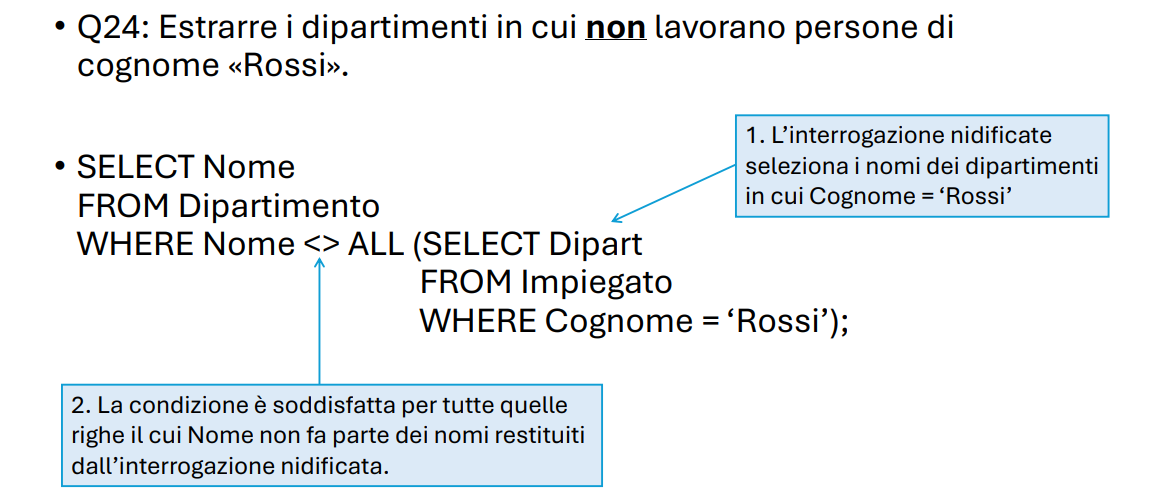
\includegraphics[width=0.5\textwidth]{images/Q24.png}
    \end{center}

    \textbf{Estrarre i dipartimenti in cui non lavorano persone di cognome Rossi}
    \begin{sqlcode}
      SELCET Nome
      FROM Diparmento
        WHERE Nome <> ALL (
          SELECT Dipart
          FROM Impiegato
            WHERE Cognome = 'Rossi'
        );
    \end{sqlcode}

    Questo equivale a:
    \begin{sqlcode}
      SELECT Nome
      FROM Dipartimento
      EXCEPT
      SELECT Dipart
      FROM Impiegato
      WHERE Cognome = 'Rossi';
    \end{sqlcode}
  \end{esempiobox}

  \vario{ATTENZIONE!}{
    Per le interrogazioni nidificate viste fino ad ora, l’interrogazione può essere eseguita una volta sola ed il risultato ottenuto può essere salvato in una tabella temporanea usata per eseguire ciascun confronto con le righe dalla tabella esterna.

    \smallskip
    Talvolta però l’interrogazione nidificata fa riferimento al contesto dell’interrogazione che la racchiude attraverso l’uso di una variabile (\textbf{passaggio di binding}).
    
    \smallskip
    L’interrogazione nidificata dovrà essere \textbf{valutata separatamente per ciascuna riga} prodotta dalla valutazione della query esterna.
  }
 
  \subsection{Clausola \texttt{EXISTS}}
   L’operatore logico $\verb|EXISTS|$ riceve come parametro un’interrogazione nidificata e restituisce il valore vero solo se l’interrogazione fornisce un risultato non vuoto.\\[0.2ex]
   Questo operatore può essere usato in modo significativo soloquando si ha un passaggio di binding tra la query esterna e quella interna.

   \begin{esempiobox}{Interrogazione con \texttt{EXISTS}}
    Consideriamo la seguente tabella:
    \begin{center}
      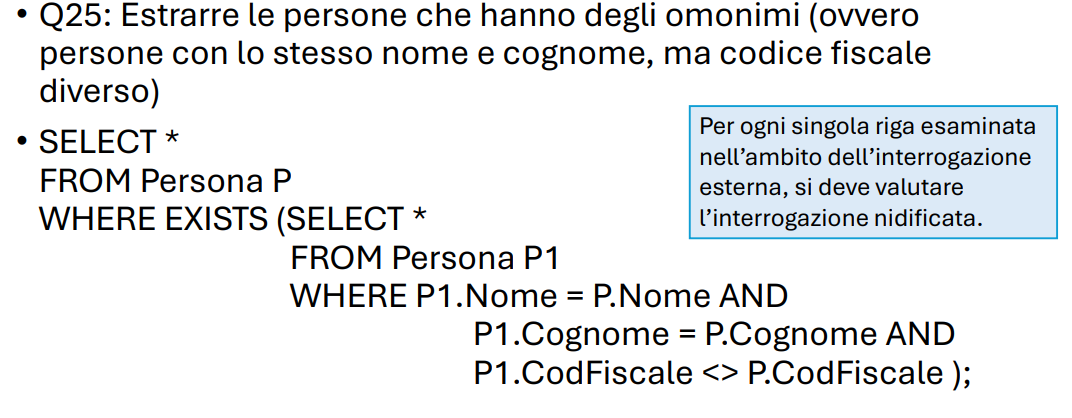
\includegraphics[width=0.5\textwidth]{images/Q25.png}
    \end{center}

    \textbf{Estrarre le persone che hanno degli omonimi (stesso nome e cognome, ma codice fiscale diverso)}
    \begin{sqlcode}
      SELECT *
      FROM Persona AS P
        WHERE EXISTS (
          SELECT *
          FROM Persona P1
          WHERE P1.Nome = P.Nome AND
            P1.Cognome = P.Cognome AND
            P1.CodFiscale <> P.CodFiscale
        );
    \end{sqlcode}
   \end{esempiobox}

  \subsection{Clausola \texttt{SELECT}}
  Le interrogazioni nidificate possono essere specificate anche come elemento della clausola $\verb|SELECT|$.

  \vario{Nota}{
     Spesso l’uso di query nidificate nella \texttt{SELECT} sostituiscono l’uso del \texttt{JOIN}.
  }

  \begin{esempiobox}{Interrogazione con \texttt{SELECT}}
    Consideriamo la seguente tabella:
    \begin{center}
       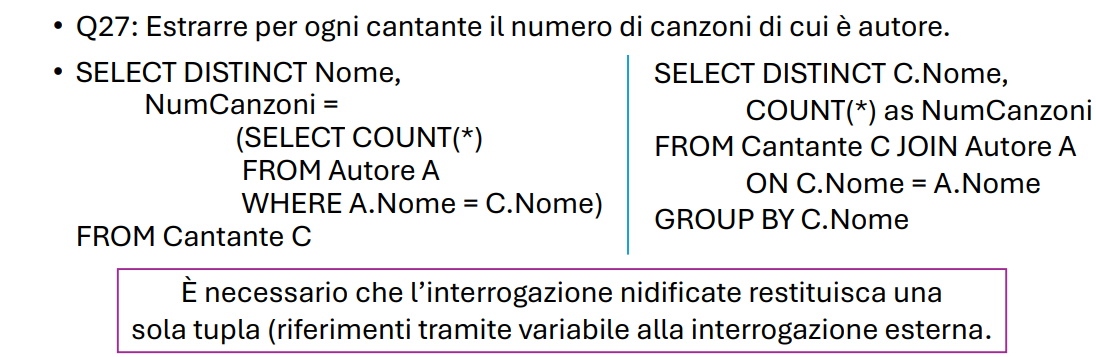
\includegraphics[width=0.5\textwidth]{images/Q27.png}
    \end{center}

    \textbf{Estrarre per ogni cantante il numero di canzoni di cui è autore}
    \begin{sqlcode}
      SELECT DISTINCT Nome, NumCanzoni = (
        SELECT COUNT(*)
        FROM Autore AS A
          WHERE A.Nome = C.Nome
      )
      FROM Cantante AS C;
    \end{sqlcode}
  \end{esempiobox}


    \subsection{Clausola \texttt{FROM}}
    Le interrogazioni nidificate possono essere utilizzate nella clausola $\verb|FROM|$ come sorgente dati su cui eseguire l’interrogazione.\\[0.2ex]
    È possibile creare una catena di interrogazioni, dove ciascuna interrogazione utilizza il risultato della precedente come una tabella di base.

    \begin{esempiobox}{Interrogazione con \texttt{FROM}}
    Consideriamo la seguente tabella:
    \begin{center}
       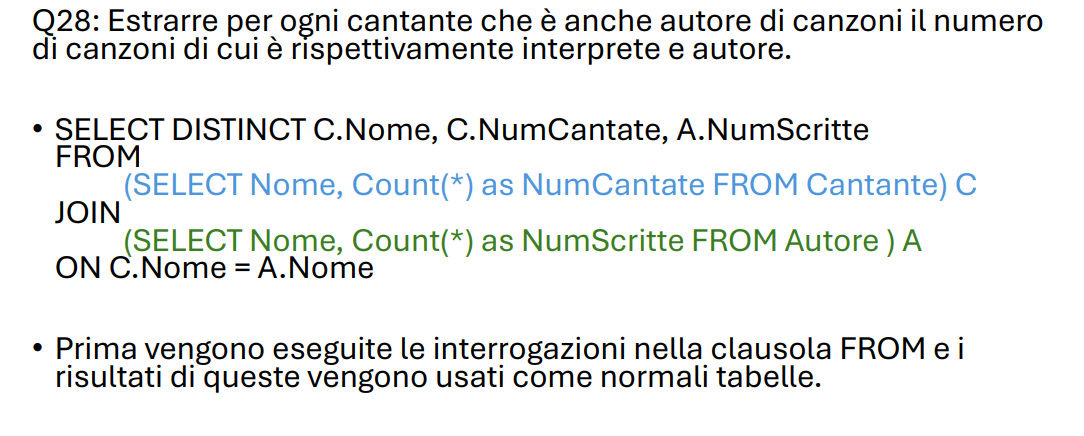
\includegraphics[width=0.5\textwidth]{images/Q28.png}
    \end{center}

    \textbf{Estrarre per ogni cantante che è anche autore di canzoni il numero di canzoni di cui è rispettivamente interprete e autore}
    \begin{sqlcode}
      SELECT DISTINCT C.NOme, C.NumCantate, A.NumScritte
      FROM (
        SELECT Nome, COUNT(*) AS NumCantate
        FROM Cantante
      ) AS C
      JOIN (
        SELECT Nome, COUNT(*) AS NumScritte
        FROM Autore
      ) AS A ON C.Nome = A.Nome;
    \end{sqlcode}
  \end{esempiobox}

 
!TeX root = BasiDiDati.tex
 
 \chapter{Strutture fisiche e di accesso ai dati}
  Le basi di dati risiedono nella \textcolor{azzurrino}{\textbf{memoria secondaria}} perchè sono:
  \begin{itemize}[label=$\triangleright$]
    \item \textbf{grandi}: non possono essere contenute completamente in memoria centrale
    \smallskip
    \item \textbf{persistenti}: hanno un tempo di vita che non è limitato all'esecuizone dei programmi che le usano
  \end{itemize}

  \vario{Caratteristiche della memoria secondaria}{
    Le caratteristiche principali della memoria secondaria sono:
    \begin{itemize}[label=$\circ$]
      \item non utilizzabile direttamente dai programmi
      \smallskip
      \item dati organizzati in \textbf{blocchi} (grandezza dipende dal sistema operativo)
      \smallskip
      \item operazioni possibili:
      \begin{itemize}[label=$\diamond$]
        \item lettura intero blocco
        \item scrittura intero blocco
      \end{itemize}
      \smallskip
      \item costo delle operazioni di accesso alla memoria secondaria è maggiore al costo per accedere ai dati in memoria centrale
    \end{itemize}
  }

  \section{Gestore del buffer}
  L'interazione tra memoria secondaria e memoria centrale avviene tramite il \textcolor{azzurrino}{\textbf{gestore del buffer}} tramite il trasferimento di uno o più \textbf{blocchi} della memoria secondaria in \textbf{pagine} dedicate della memoria centrale (buffer).

  \vario{Precisazione}{
    La dimensione delle pagine in memoria centrale sono siltamente un multiplo della dimensione dei blocchi in memoria secondaria.

    \smallskip
    Per semplificare, si assume che siano uguali:
    \begin{equation*}
      \text{1 pagina} \approx \text{1 blocco}
    \end{equation*}
  }

  \subsection{Buffer}
  Il \textcolor{azzurrino}{\textbf{buffer}} è una zona della memoria condivisa dalle applicazioni e una gestiona ottimale del buffer consente di ottenere buone prestazioni nell'accesso ai dati.\\[0.2ex]
  Quando uno stesso dato viene utilizzato più volte in tempi ravvicinati il buffer evita
  l’accesso alla memoria secondaria.

  \vario{Compito del gestore del buffer}{
    Il gestore del buffer si occupa del caricare e salvare i dati dalla memoria secondaria alla memoria centrale.
  }

  \subsection{Politica di gestione della memoria}
  L'obiettivo del gestore del buffer è di \hl{ottimizzare gli accessi} attraverso le politiche di gestione della memoria:
  \begin{itemize}[label=$\diamond$]
    \item \textbf{lettura di un blocco}:
    \begin{itemize}[label=$\triangleright$]
      \item blocco presente in una pagina del buffer
      \begin{itemize}[label=$\Rightarrow$]
        \item non viene eseguita la lettura in memoria secondaria
        \smallskip
        \item viene restituito un puntatore alla pagine del buffer
      \end{itemize}
      \medskip
      \item blocco non presente in una pagina del buffer
      \begin{itemize}[label=$\Rightarrow$]
        \item viene cercata una pagina libera
        \smallskip
        \item viene caricato il blocco nella pagina
        \smallskip
        \item viene restituito il puntatore alla pagina del buffer
      \end{itemize}
    \end{itemize}
    \bigskip
    \item \textbf{scrittura di un blocco}: se viene effettuata una richiesta si dcrittura di un blocco giù caricato in una pagina del buffer, il gestore del buffer può decidere di \hl{differire la scrittura} su memoria secondaria in un secondo momento
  \end{itemize}

  \medskip
  Per poter aumentare la velocità di accesso ai dati, le politiche di lettura e scrittura si basano sul \textbf{principio di località}.

  \definizione{principio di località}{
    Il \textbf{principio di località} si basa sul fatto che i dati refernziati di recente hanno maggiore probabilità di essere referenziati nuovamente in futuro.
  }

  \subsection{Gestione delle pagine}
  Il contenuto del buffer lo possiamo immaginare come una matrice.

  \begin{figure}[H]
    \centering
    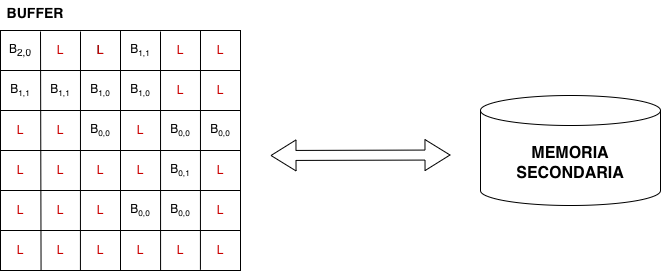
\includegraphics[width=0.5\textwidth]{images/gestione-pagine.png}
  \end{figure}

  Per ogni pagina del buffer si memorizza:
  \begin{itemize}[label=$\triangleright$]
    \item blocco B (L se libero) indicando il file e il numero di blocco (offset)
    \smallskip
    \item variabili di stato ($B_{i,j}$):
    \begin{itemize}[label=$\circ$]
      \item contatore i: indica il numero di transazioni
      \item bit di stato j: indica se la pagina è stata modificata (1) o no (0)
    \end{itemize}
  \end{itemize}

  \subsection{Primitive per la gestione del buffer}

  \subsubsection{Primitiva \protect\texttt{fix}}
  La \textcolor{azzurrino}{primitiva \texttt{fix}} viene utilizzata dalle transazioni per richiedere l'accesso ad un blocco e restituisce un puntatore alla pagina contente il blocco richiesto.

  Le azioni della primitiva sono:
  \begin{itemize}[label=$\triangleright$]
    \item \textbf{ricerca del blocco}:
    \begin{itemize}[label=$\diamond$]
      \item blocco viene trovato
      \begin{itemize}[label=$\Rightarrow$]
        \item viene restituito un puntatore alla pagina contentente il blocco
      \end{itemize}
      \medskip
      \item blocco non viene trovato:
      \begin{itemize}[label=$\circ$]
        \item viene scelta una pagina libera
        \begin{itemize}[label=$\Rightarrow$]
          \item viene salvata in memoria secondaria (primitiva $\verb|flush|$)
          \item viene caricato il blocco in P aggiornando file e numero di blocco
        \end{itemize}
        \smallskip
        \item non ci sono pagine libere
        \begin{itemize}[label=$\Rightarrow$]
          \item viene rubata una pagina a un'altra transazione (primitiva $\verb|flush|$)
          \item viene sospesa la transazione inserendola in una cosa di attesa
          \item se si libera una pagina il gestore si comporterà come al punto precedente
        \end{itemize}
      \end{itemize}
    \end{itemize}
  \end{itemize}

  \medskip
  \begin{itemize}[label=$\Rightarrow$]
    \item \textbf{effetto della modifica}: quando una transizione accede a una pagina per la prima volta il contatore si incrementa
  \end{itemize}

  \subsubsection{Primitiva \protect\texttt{unfix}}
  La \textcolor{azzurrino}{primitiva \texttt{unfix}} viene usata dalle transazioni per indicare che la transazione ha terminato di usare il blocco.

  \begin{itemize}[label=$\Rightarrow$]
    \item \textbf{effetto della modifica}: decremento del contatore i
  \end{itemize}

  \subsubsection{Primitiva \protect\texttt{setDirty}}
  La \textcolor{azzurrino}{primitiva \texttt{setDirty}} viene utilizzata dalle transazioni per indicare al gestore del buffer che il blocco della pagina è stato modificato.

  \begin{itemize}[label=$\Rightarrow$]
    \item \textbf{effetto della modifica}: bit di stato J passa da 0 a 1
  \end{itemize}

  \subsubsection{Primitiva \protect\texttt{force}}
  La \textcolor{azzurrino}{primitiva \texttt{force}} viene utilizzata per salvare in memoria secondaria in \hl{modo sincrono} il blocco contenuto nella pagina.\\[0.2ex]
  Questa primitiva viene usata dal gestore dell'affidabilità.

  \begin{itemize}[label=$\Rightarrow$]
    \item \textbf{effetto della modifica}: viene salvato in memoria secondaria il blocco e il bit di stato J posto a 0
  \end{itemize}

  \subsubsection{Primitiva \protect\texttt{flush}}
  La \textcolor{azzurrino}{primitiva \texttt{flush}} viene utilizzata per salvare i blocchi in memoria secondaria in \hl{modo asincrono}.\\[0.2ex]
  Questa primitiva viene usata dal gestore del buffer.

  \begin{itemize}[label=$\Rightarrow$]
    \item \textbf{effetto della modifica}: viene liberta la pagina "dirty" e il bit di stato J viene posto a 0
  \end{itemize}

  \section{Gestore dell'affidabilità}
  Il gestore del buffer differisce le operazioni di scrittura e questo potrebbe raprresentare un pericolo.\\[0.2ex]
  Il \textcolor{azzurrino}{\textbf{gestore dell'affibilità}} si occupa di garantire:
  \begin{itemize}[label=$\triangleright$]
    \item \textbf{atomicità}: transazioni non devono essere incomplete
    \smallskip
    \item \textbf{persistenza}: effetti di ciascuna transazione non conclusa con un commit devono essere mantenuti in modo permanente
  \end{itemize}

  \begin{figure}[H]
    \centering
    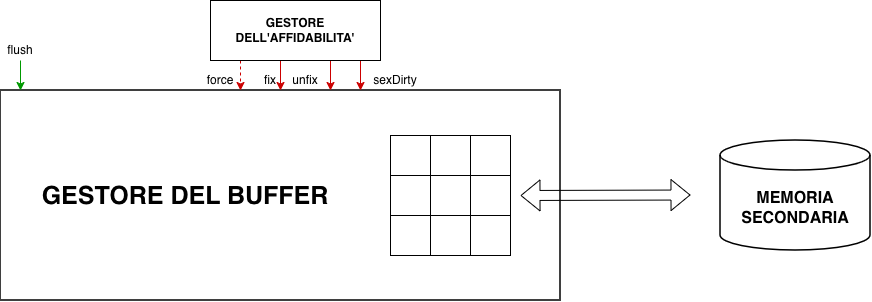
\includegraphics[width=0.6\textwidth]{images/gestore-affidabilità.png}
  \end{figure}


  \subsection{File di LOG}
  Il funzionamento del gestore dell'affidabilità si basa sull'utilizzo del \textbf{file di LOG}.

  \definizione{file di LOG}{
    Il \textbf{file di LOG} è un archivio persistente su cui vengono registrate tutte le operazioni eseguite dal DBMS.
  }

  Per il corretto funzionamento, il gestore dell’affidabilità deve disporre di un dispositivo di una \textbf{memoria stabile} (resistente ai guasti).

  Il file di LOG viene memorizzato in memoria stabile e al suo interno vengono memorizzati:
  \begin{itemize}[label=$\triangleright$]
    \item \textbf{record di transizione}: record che descrivono informazioni sulle transazioni
    \begin{itemize}[label=$\diamond$]
      \item $\boldsymbol{\mathrm{B(T)}}$: \textcolor{azzurrino}{\textbf{begin}} della transazione
      \smallskip
      \item $\boldsymbol{\textbf{C(T)}}$: \textcolor{azzurrino}{\textbf{commit}} della transazione
      \smallskip
      \item $\boldsymbol{\textbf{A(T)}}$: \textcolor{azzurrino}{\textbf{abort}} della transazione
      \smallskip
      \item $\boldsymbol{\textbf{I(T,O,AS)}}$: \textcolor{azzurrino}{\textbf{insert}} di un oggetto da parte di una transazione $\mathrm{T}$ con il suo after state $\mathrm{AS}$ (stato dell'oggetto dopo l'operazione)
      \smallskip
      \item $\boldsymbol{\mathrm{D(T,O,BS)}}$: \textcolor{azzurrino}{\textbf{delete}} di un oggetto $\mathrm{O}$ da parte della transizione $\mathrm{T}$ con il suo before state $\mathrm{BS}$ (stato dell'oggetto prima dell'operazione)
      \smallskip
      \item $\boldsymbol{\mathrm{U(T,O,BS,AS)}}$: \textcolor{azzurrino}{\textbf{update}} di un oggetto $\mathrm{O}$ da parte della transizione $\mathrm{T}$ con il suo before state $\mathrm{BS}$ e il suo after state $\mathrm{AS}$
    \end{itemize}
    \medskip
    \item \textbf{record di sistema}: record che descrivono informazioni sulle operazioni esaguite dal DBMS
    \begin{itemize}[label=$\circ$]
      \item $\boldsymbol{\mathrm{DUMP}}$: copia completa e consistente della base di dati.
      \smallskip
      \item $\boldsymbol{\mathrm{CK}(T_1, \dots, T_n)}$: indica che all'esecuzione del checkpoint, le transazioni attive erano $T_1, \dots, T_n$
      \begin{itemize}
        \item elenco delle transazioni che non hanno ancora espresso la loro scelta relativamente all'esito finale
        \smallskip
        \item operazione svolta periodicamente affinché i dati delle transazioni che hanno eseguito il \texttt{commit} siano registrati in modo permanente
        \smallskip
        \item il protocollo di checkpoint prevede i seguenti passi:
        \begin{enumerate}
          \item sospensione delle operazioni di scrittura, \texttt{commit} e \texttt{abort} delle transazioni
          \smallskip
          \item esecuzione della primitiva \texttt{force} sulle pagine ``dirty'' di transazioni che hanno eseguito il \texttt{commit}
          \smallskip
          \item scrittura sincrona (primitiva \texttt{force}) sul file di LOG del record di checkpoint con gli identificatori delle transazioni attive
          \smallskip
          \item ripresa delle operazioni di scrittura, \texttt{commit} e \texttt{abort} delle transazioni
        \end{enumerate}
      \end{itemize}
    \end{itemize}
  \end{itemize}

I record di transazione salvati nel LOG consentono di eseguire in caso di ripristino le seguenti operazioni:
\begin{itemize}[label=$\triangleright$]
  \item $\boldsymbol{\mathrm{UNDO}}$: viene usato per disfare un'azione su un oggetto $\mathrm{O}$ è sufficiente ricopiare in $\mathrm{O}$ il valore d $\mathrm{BS}$.
  
  L'insert/delet viene disfatto cancellando/inserendo $\mathrm{O}$
  \smallskip
  \item $\boldsymbol{\mathrm{REDO}}$: serve per rifare un'azione su un oggetto $\mathrm{O}$ è sufficiente ricopiare in $\mathrm{O}$ il valore $\mathrm{AS}$.
  
  L'insert/delete viene rifatto inserendo/cancellando $\mathrm{O}$
\end{itemize}

\medskip
Gli inserimenti controllano sempre l’esistenza di $\mathrm{O}$ prima di eseguire l'operazione.\\[0.2ex]
Per queste operazioni vale la \textbf{proprietà di idempotenza}.

\definizione{proprietà di idempotenza}{
  \[
    \begin{aligned}
      \mathrm{UNDO(UNDO(A))} &= \mathrm{UNDO(A)}\\
      \mathrm{REDO(REDO(A))} &= \mathrm{REDO(A)}
    \end{aligned}
  \]
}

\subsection{Regole di scrittura sul file di log}
Il gestore dell'affibilità deve rispettare le seguenti regole di scrittura sul file di LOG:
\begin{itemize}[label=$\Rightarrow$]
  \item \textbf{regola Write Ahead Logging}:record di LOG devono essere scritti sul LOG precedente all'esecuzione delle corrispondenti operazioni sulla base di dati (garantisce la possibilità di fare sempre UNDO)
  \smallskip
  \item \textbf{regola di commit-precedenza}: record di LOG devono essere scritti sul LOG prima dell'esecuzione del $\texttt{commit}$ della transazione (garantisce la possibilità di fare sempre REDO)
\end{itemize}

 Queste regole consentono di salvare i blocchi delle pagine “dirty” in modo totalmente asincrono rispetto al commit delle transazioni.

\subsection{Guasti}
Una transazione T sceglie in modo atomico l’esito di $\verb|commit|$ nel momento in cui
scrive nel file di log in modo sincrono (primitiva $\verb|force|$) il suo record di $\verb|commit| \ \mathrm{C(T)}$. 

\begin{itemize}[label=$\Rightarrow$]
  \item se avviene un guasto prima della scrittura del record di $\verb|commit|$ $\rightarrow$ $\boldsymbol{\mathrm{UNDO}}$
  \smallskip
  \item se avviene un guasto dopo la scrittura del record di $\verb|commit|$ $\rightarrow$ $\boldsymbol{\mathrm{REDO}}$
\end{itemize}

Esistono due tipologie di guasto:
\begin{itemize}[label=$\triangleright$]
  \item \textbf{guasto di sistema}: perdita del conte della memoria centrale.
  
  Viene risolto con la tecnica della \hl{ripresa a caldo}:
  \begin{enumerate}
    \item accede al file di LOG e si ripercorre all’indietro il LOG fino al più recente record di checkpoint
    \smallskip
    \item si inizializza:
    \begin{itemize}[label=$\diamond$]
      \item insieme $\mathrm{UNDO}$ con tutte le transazioni da disfare (presenti nel checkpoint)
      \smallskip
      \item insieme $\mathrm{REDO}$ con tutte le transazioni da rifare ($\emptyset$)
    \end{itemize}
    \smallskip
    \item si ripercorre in avanti il LOG
    \begin{itemize}[label=$\circ$]
      \item per ogni record $\mathrm{B(T)}$ incontrato si aggiunge T all’insieme $\mathrm{UNDO}$
      \smallskip
      \item per ogni record $\mathrm{C(T)}$ incontrato si sposta T dall’insieme $\mathrm{UNDO}$ all’insieme $\mathrm{REDO}$
    \end{itemize}
    \smallskip
    \item si ripercorre all’indietro il LOG disfacendo le operazioni eseguite dalle transazioni $\mathrm{UNDO}$ risalendo fino alla prima azione della transazione più vecchia
    \item si ripercorre in avanti il LOG per rifare le operazioni eseguite dalle transazioni $\mathrm{REDO}$
  \end{enumerate}
  \medskip
  \item \textbf{guasto di dispositivo}: perdita di parte o tutto il contenuto della base di dati in memoria secondaria.
  
  Viene risolto con la tecninca della \hl{ripresa a freddo}:
  \begin{enumerate}
    \item si accede al $\mathrm{DUMP}$ della base di dati e si ricopia selettivamente la parte deteriorata della base di dati
    \smallskip
    \item si accede al LOG risalendo al record di $\mathrm{DUMP}$
    \smallskip
    \item si ripercorre in avanti il LOG rieseguendo tutte le operazioni relative alla perte deteriorata comprese le azioni di $\verb|commit|$ e $\verb|abort|$
    \smallskip
    \item si applica una ripresa a caldo
  \end{enumerate}
\end{itemize}

\esempio{file di LOG}{
  Consideriamo il seguente file di LOG:
  \[
    \begin{aligned}
      & \mathrm{B(T_1), B(T_2), U(T_2, O_1, B_1, A_1), I(T_1, O_2, A_2), B(T_3), C(T_1), B(T_4),} \\
      & \mathrm{U(T_3, O_2, B_3, A_3), U(T_4, O_3, B_4, A_4), CK(T_2, T_3, T_4), C(T_4), B(T_5),} \\
      & \mathrm{U(T_3, O_3, B_5, A_5), U(T_5, O_4, B_6, A_6), D(T_3, O_5, B_7), A(T_3), C(T_5),} \\
      & \mathrm{I(T_2, O_6, A_8)} \text{ \textbf{guasto}}
    \end{aligned}
  \] 

  \textcolor{red}{\textbf{Che passi svolge la ripresa a caldo?}}
  \begin{enumerate}
    \item risale il LOG fino all'ultimo record di checkpoint $\mathrm{CK(T_2,T_3,T_4)}$
    \smallskip
    \item inizializza $\mathrm{UNDO}$ e $\mathrm{REDO}$
    \begin{itemize}[label=$\triangleright$]
      \item $\mathrm{UNDO = \{T_2, T_3, T_4\}}$ (inizializzato con le transazioni del checkpoint)
      \smallskip
      \item $\mathrm{REDO = \emptyset}$ 
    \end{itemize}
    \smallskip
    \item ripercorre in avanti il LOG dal CheckPoint fino al guasto e si aggiungono o si spostano le transazioni tra $\mathrm{UNDO}$ e $\mathrm{REDO}$
    \begin{itemize}[label=$\triangleright$]
      \item $\mathrm{UNDO = \{T_2, T_3, \cancel{T_4}, \cancel{T_5}\}}$ (inizializzato con le transazioni del checkpoint)
      \smallskip
      \item $\mathrm{REDO = \{T_4, T_5\}}$ 
    \end{itemize}
    \smallskip
    \item ripercorre all’indietro il LOG disfacendo le operazioni eseguite dalle transazioni $\mathrm{UNDO}$ risalendo fino alla prima azione della transazione più vecchia
    \[
      \begin{aligned}
        &\mathrm{DELETE(O_6) \quad (\text{disfare} \ \texttt{insert})}\\
        &\mathrm{O_5 := B_7  \quad (\text{disfare} \ \texttt{delete})}\\
        &\mathrm{O_3 := B_5 \quad (\text{disfare} \ \texttt{update})}\\
        &O_2 := B_3 \ \quad (\text{disfare} \ \texttt{update})\\
        &\mathrm{O_1 := B_1 \quad (\text{disfare} \ \texttt{update})}\\
      \end{aligned}
    \]
    \smallskip
    \item  ripercorre in avanti il LOG per rifare le operazioni eseguite dalle transazioni $\mathrm{REDO}$
    \[
      \begin{aligned}
        &\mathrm{O_3 := A_4  \quad (\text{rifare} \ \texttt{update})}\\
        &\mathrm{O_4 := A_6 \quad (\text{rifare} \ \texttt{update})}\\
      \end{aligned}
    \]
  \end{enumerate}
}

\esempio{file di LOG}{
  Consideriamo il seguente file di LOG:
  \[
    \begin{aligned}
      &\mathrm{B(T_1), B(T_2), B(T_3), I(T_1, O_1, A_1), D(T_2, O_2, B_2), B(T_4),} \\
      &\mathrm{U(T_4, O_3, B_3, A_3), U(T_1, O_4, B_4, A_4), C(T_2), CK(T_1, T_3, T_4), B(T_5), B(T_6),} \\
      &\mathrm{U(T_5, O_5, B_5, A_5), A(T_3), CK(T_1, T_4, T_5, T_6), B(T_7), C(T_4),} \\
      &\mathrm{U(T_7, O_6, B_6, A_6), U(T_6, O_3, B_7, A_7), B(T_8), A(T_7)} \text{ \textbf{guasto}}
    \end{aligned}
  \]

  \textcolor{red}{\textbf{Che passi svolge la ripresa a caldo?}}
  \begin{enumerate}
    \item risale il LOG fino all'ultimo record di checkpoint $\mathrm{CK(T_1,T_4,T_5,T_6)}$
    \smallskip
    \item inizializza $\mathrm{UNDO}$ e $\mathrm{REDO}$
    \begin{itemize}[label=$\triangleright$]
      \item $\mathrm{UNDO = \{T_1, T_4, T_5, T_6\}}$ (inizializzato con le transazioni del checkpoint)
      \smallskip
      \item $\mathrm{REDO = \emptyset}$ 
    \end{itemize}
    \smallskip
    \item ripercorre in avanti il LOG dal CheckPoint fino al guasto e si aggiungono o si spostano le transazioni tra $\mathrm{UNDO}$ e $\mathrm{REDO}$
    \begin{itemize}[label=$\triangleright$]
      \item $\mathrm{UNDO = \{T_1, \cancel{T_4}, T_5, t_6, t_7, t_8\}}$ (inizializzato con le transazioni del checkpoint)
      \smallskip
      \item $\mathrm{REDO = \{T_4\}}$ 
    \end{itemize}
    \smallskip
    \item ripercorre all’indietro il LOG disfacendo le operazioni eseguite dalle transazioni $\mathrm{UNDO}$ risalendo fino alla prima azione della transazione più vecchia
    \[
      \begin{aligned}
        &\mathrm{O_3 := B_7  \quad (\text{disfare} \ \texttt{update})}\\
        &\mathrm{O_6 := B_6 \quad (\text{disfare} \ \texttt{update})}\\
        &\mathrm{O_5 := B_5 \quad (\text{disfare} \ \texttt{update})}\\
        &\mathrm{O_4 := B_4  \quad (\text{disfare} \ \texttt{update})}\\
        &\mathrm{DELETE(O_1) \quad (\text{disfare} \ \texttt{insert})}\\
      \end{aligned}
    \]
    \smallskip
    \item  ripercorre in avanti il LOG per rifare le operazioni eseguite dalle transazioni $\mathrm{REDO}$
    \[
      \begin{aligned}
        &\mathrm{O_3 := A_3  \quad (\text{rifare} \ \texttt{update})}\\
      \end{aligned}
    \]
  \end{enumerate}
}

\section{Gestore dei metodi di accesso}
Il gestore dei metodi di accesso esegue il piano di esecuzione prodotto dall'ottimizzatore e produce sequenze richieste di accessi ai blocchi della base di dati presenti in memoria secondaria.\\[0.2ex]
Le richieste vengono inviate al gestore del buffer che si occupa di caricare i blocchi necessari in pagine di memoria centrale.

\begin{figure}[H]
  \centering
  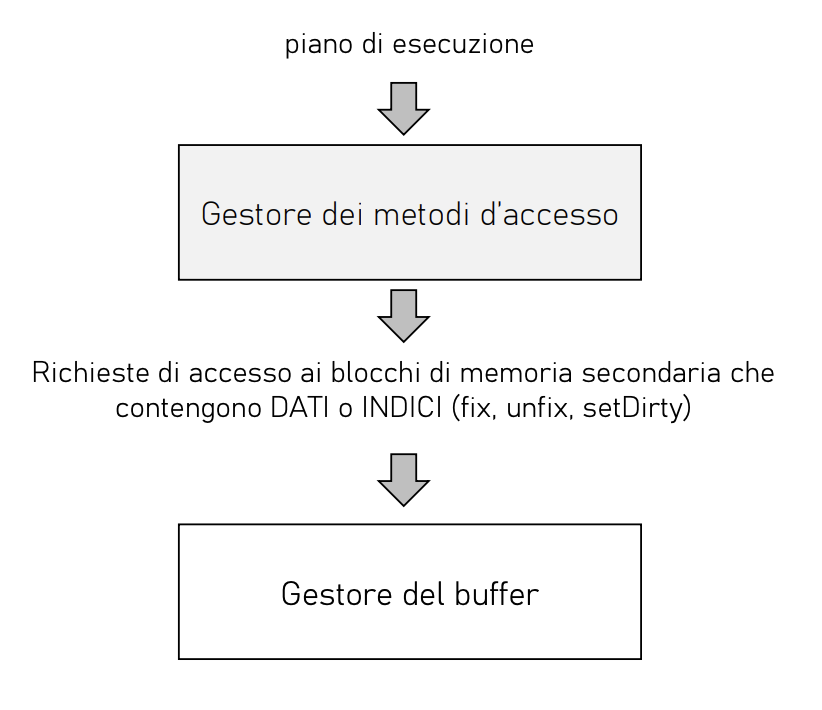
\includegraphics[width=0.6\textwidth]{images/gestore-accesso.png}
  \caption{gestore dei meotodi di accesso}
\end{figure}

\subsection{Metodi di accesso}
I metodi di accesso sono moduli software (es. scansione sequenziale, accesso via indice, ordinamento, varie implementazioni del join) che implementano gli algoritmi di accesso e manipolazione dei dati organizzati in specifiche strutture fisiche.

Ogni metodo di accesso conosce:
\begin{itemize}[label=$\diamond$]
  \item \textbf{organizzazione in tuple} (o dei record di indice) nei blocchi dati (indice) salavati in memoria secondaria
  \smallskip
  \item \textbf{organizzazione fisica interna delle pagine} sia quando contengono dati, sia quando contengono strutture fisiche di accesso (indici)
\end{itemize}

\subsection{Organizzazione di una pagina}
All'interno di una pagina sono presenti:
\begin{itemize}[label=$\triangleright$]
  \item \textbf{informazioni utili}: dati veri e propri (tuple della tabella)
  \smallskip
  \item \textbf{informazioni di controllo}: consentono di accedere alle informazioni utili (dizionario, bt di parità, altre informazioni del file system o della specifica struttura fisica)
\end{itemize}

\begin{figure}[H]
  \centering
  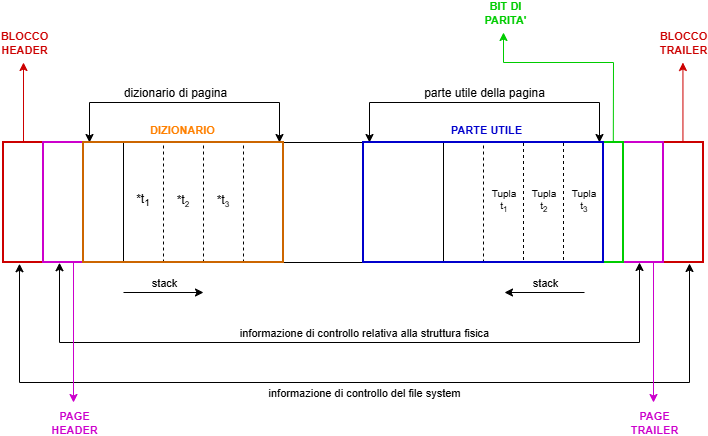
\includegraphics[width=0.6\textwidth]{images/organizzazione-pagina.png}
  \caption{organizzazione di una pagina}
\end{figure}

\begin{itemize}[label=$\Rightarrow$]
  \item \textcolor{red}{\textbf{blocco header/trailer}}: contengono informazioni di controllo utilizzate daò file system
  \smallskip
  \item \textcolor{violet}{\textbf{pagina header/trailer}}: contengono le informazioni di controllo relative alla specifica struttura fisica
  \smallskip
  \item \textcolor{orange}{\textbf{dizionario di pagina}}: contiene i puntatori a ciascun dato utile elementare contenuto nella pagina
  \smallskip
  \item \textcolor{green}{\textbf{bit di parità}}: verifica che l'informazione contenuta nella pagina sia valida
  \smallskip
  \item \textcolor{blue}{\textbf{parte utile}}: contiene i dati
\end{itemize}

\vario{N.B.}{
  Dizionari di pagina e parte utile crescono come stack contrapposti, lasciando libera la parte centrale in uno spazio contiguo.
}

In caso di \textbf{tuple di lunghezza fissa}, il dizionario non è necessario: si memorizza la dimensione delle tutple e l'offset del punto iniziale.\\[0.2ex]
In caso di di \textbf{tuple di lunghezza variabile}, il dizionario memorizza l'offset di ogni tupla presente nel blocco e di ogni attributo di ogni tupla.

Molti gestori delle pagine non consentono la separazione di una tupla su più pagine:
\begin{equation*}
  \text{dimensione massima tupla} = \text{dimensione massima area disponibile su un blocco}
\end{equation*}

Alcuni gestori delle pagine consentono di distribuire una tupla su più pagine, altrimenti va gestito il caso di tuple memorizzato su più pagine.

\subsection{Operazioni sulle pagine}
Le princpali operazioni che si possono eseguire sulle pagine sono:
\begin{itemize}[label=$\triangleright$]
  \item \textbf{inserimento/aggiornamento di una tupla}:
  \begin{itemize}[label=$\diamond$]
    \item esiste spazio contiguo sufficiente: Inserimento
    \smallskip
    \item non esiste spazio contiguo sufficiente, ma spazio sufficiente: riorganizzazione dello spazio + inserimento
    \smallskip
    \item non esiste spazio sufficiente: interazione con il file system per allocare nuovi blocchi per il file
  \end{itemize}
  \smallskip
  \item \textbf{cancellazione contenuto della pagina}
  \smallskip
  \item \textbf{accesso a una tupla}: avviene tramite il valore della chiave o l'offset nel dizionario
  \smallskip
  \item \textbf{accesso a un attributo di una tupla}: identificato in base all’offset e alla lunghezza del campo dopo aver identificato la tuplatramite la chiave o il suo offset 
\end{itemize}


\subsection{Strutture primarie per l'organizzazione dei file}
La struttura prmaria di un file stabilisce il criterio di disposizione delle tuple all'interno del file presente in memoria di massa:
\begin{itemize}[label=$\triangleright$]
  \item \textbf{sequenziale}: colloca le tuple in maniera consecutiva sulla base di un criterio specifico (es. ordine di inserimento)
  \smallskip
  \item \textbf{ad accesso clacolato}: colloca le tuple in posizioni determinate sulla base dell'esecuzione di un algoritmo di hash
  \smallskip
  \item \textbf{ad albero}: utilizzate come strutture secondarie (indici)
\end{itemize}

\begin{figure}[H]
  \centering
  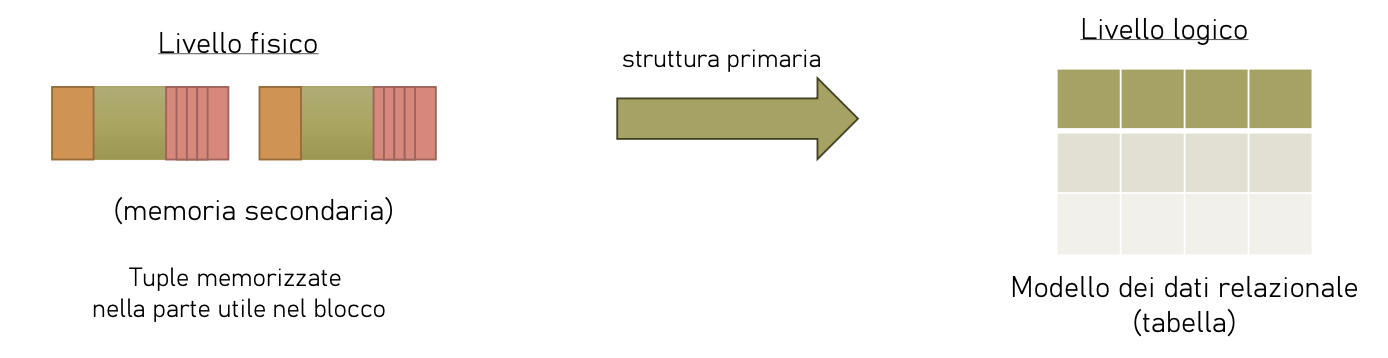
\includegraphics[width=0.6\textwidth]{images/strutture-primarie.png}
  \caption{strutture primarie per l'organizzazione dei file}
\end{figure}

\subsubsection{Struttura sequenziale}
Un file è costituito da blocchi "logicamente" consecutivi e le tuple vengono inserite nei blocchi rispettando una sequenza.

\paragraph{Struttura sequenziale disordinata}
Le tuple sono disposte in
base al loro ordine di inserimento, senza alcun criterio specifico.\\[0.2ex]
Questa è la
struttura più semplice e più diffusa.

\begin{itemize}[label=$\Rightarrow$, itemsep=\smallskipamount]
  \item \textbf{inserimento}:
  \begin{itemize}[label=$\diamond$, itemsep=\smallskipamount]
    \item operazione molto efficiente
    \item sufficiente mantenere uun riferimento all'ultimo blocco
    \item richiede solo un accesso in memoria secondaria
    \item maggiore costo in caso di verifica dei vincoli di integrità
  \end{itemize}
  \item \textbf{ricerca}
  \begin{itemize}[label=$\diamond$, itemsep=\smallskipamount]
    \item operazione non efficiente
    \item richiede ogni volta una scansione sequenziale che consideri tutti i record, con un costo lineare nel numero di blocchi
    \item ricerca può essere fatta usando strutture secondarie (indici)
  \end{itemize}
  \item \textbf{eliminazione}
  \begin{itemize}[label=$\diamond$, itemsep=\smallskipamount]
    \item  facile una volta individuate le tuple coinvolte
    \item si marcano le tuple come "cancellate" senza riorganizzazione locale
  \end{itemize}
  \item \textbf{modifica}
  \begin{itemize}[label=$\diamond$, itemsep=\smallskipamount]
    \item  facile una volta individuate le tuple coinvolte
    \item si procede in loco se possibile, cioè quando non c’è stata nessuna modifica alla dimensione della tupla
    \item si procede con una cancellazione e un inserimento in fondo al file
  \end{itemize}
\end{itemize}

Eliminazioni e modifiche possono portare ad un uso non ottimale dello spazio
siccome si devono effettuare riorganizzazioni periodiche.

\paragraph{Struttura sequenziale ad array}
Le tuple sono disposte come in un array, e la loro posizione dipende dal valore assunto in ciascuna tupla da un campo detto \textbf{indice}.\\[0.2ex]
Questa struttura è utilizzabile soltanto quando le tuple di una tabella
hanno una dimensione fissa, infatti non è quasi masi usata nei DBMS reali perchè difficilmente sono soddisfatte le condizioni per la sua applicazione.

Ad ogni file viene assegnato un numero n di blocchi contigui e ciascun blocco
è dotato di un numero m di posizioni disponibili per le tuple (quindi è un
array bidimensionale n × m).\\[0.2ex]
Ogni tupla è dotata di un valore numerico i
che rappresenta l’indice della tupla in i-esima posizione nell’array.

\begin{itemize}[label=$\Rightarrow$, itemsep=\smallskipamount]
  \item \textbf{inserimento}
  \begin{itemize}[itemsep=\smallskipamount]
    \item Iniziale: l’indice i viene ottenuto incrementando un contatore
    \item Successivo: in una posizione libera oppure alla fine del file
  \end{itemize}
  \item \textbf{cancellazione}: creano delle posizioni libere
\end{itemize}

\paragraph{Struttura sequenziale ordinata}
È un file sequenziale dove le tuple sono ordinate secondo una chiave di ordinamento (diversa dalla chiave primaria).\\[0.2ex]
Questa struttura rende efficienti le operazioni che hanno bisogno
dell’ordinamento utilizzato, ad esempio:
\begin{itemize}[label=$\circ$, itemsep=\smallskipamount]
  \item elenco ordinato
  \item range query
  \item operazioni aggregate
\end{itemize}

In caso di aggiornamento è necessario mantenere l’ordinamento, quindi servono periodiche riorganizzazioni.

\begin{itemize}[label=$\Rightarrow$, itemsep=\smallskipamount]
  \item \textbf{inserimento}
  \begin{enumerate}[itemsep=\smallskipamount]
    \item individuare il blocco B che contiene la tupla che precede, nell’ordine della chiave, la tupla da inserire
    \item se B contiene spazio sufficiente per la nuova tupla allora si inserisce la tupla in B
    \item altrimenti si aggiunge un nuovo blocco, detto overflow page, alla struttura e si inserisce la tupla nel nuovo blocco e si aggiusta la catena di puntatori
  \end{enumerate}
  \item \textbf{scansione sequenziale ordinata secondo la chiave}:  è sufficiente seguire i puntatori
  \item \textbf{cancellazione di una tupla}
  \begin{enumerate}[itemsep=\smallskipamount]
    \item individuare il blocco B che contiene la tupla da cancellare
    \item Cancellare la tupla da B
    \item aggiustare la catena di puntatori
  \end{enumerate}
  \item \textbf{riorganizzazione}: si assegnano le tuple ai blocchi in base ad opportuni coefficienti di riempimento, riaggiustando i puntatori
\end{itemize}

\esempio{struttura sequenziale}{
  Il seguente esempio mostra una struttura sequenziale ordinata secondo la chiave $\texttt{Filiale}$.
  
  \begin{figure}[H]
    \centering
    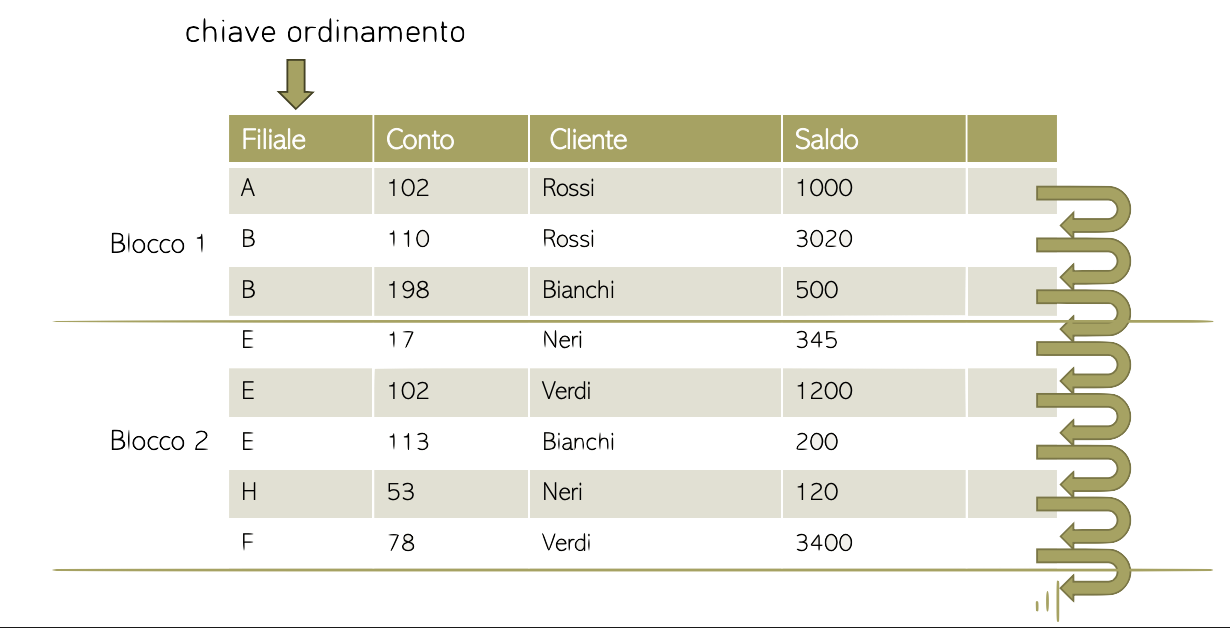
\includegraphics[width=0.6\textwidth]{images/esempio-struttura-sequenziale.png}
  \end{figure}
}

\paragraph{Indice}
Per aumentare le prestazioni degli accessi alle tuple memorizzate nelle strutture fisiche (file sequenziale), si introducono strutture ausiliarie dette strutture di accesso
ai dati, o indici.\\[0.2ex]
Queste strutture velocizzano l’accesso casuale via chiave di ricerca, cioè un insieme di attributi utilizzati nell’indice della ricerca.

Ci sono due tipi di indici su file sequenziali:
\begin{itemize}[label=$\triangleright$, itemsep=\smallskipamount]
  \item \textbf{indice primario}: la chiave di ordinamento del file sequenziale coincide con la chiave di ricerca dell’indice.
  
  Ogni record dell’indice primario contiene una coppia $\langle v_i, p_i\rangle$, dove:
  \begin{itemize}
    \item $v_i$ è il valore della chiave di ricerca
    \item $p_i$ è il puntatore al primo record nel file sequenziale con chiave $v_i$
  \end{itemize}

  Esistono due varianti dell’indice primario:
  \begin{itemize}[itemsep=\smallskipamount]
    \item \textbf{indice denso}: per ogni occorrenza della chiave presente nel file esiste un corrispondente record nell’indice
    \item \textbf{indice sparso}: solo per alcune occorrenze della chiave presenti nel file esiste un corrispondente record nell’indice, tipicamente una per blocco
  \end{itemize}

  Le operazioni che si possono eseguire su un indice primario sono:
  \begin{itemize}
    \item \textbf{ricerca} di una tupla con chiave di ricerca K
    \begin{itemize}
      \item Se l’indice è denso K è presente nell’indice
      \begin{enumerate}
        \item Scansione sequenziale dell’indice per trovare il record (K, pk)
        \item Accesso al file attraverso il puntatore pk
      \end{enumerate}

      Il costo è 1 accesso indice + 1 accesso blocco dati
      \item Se l’indice è sparso K potrebbe non essere presente nell’indice
      \begin{enumerate}
        \item Scansione sequenziale dell’indice fino al record $(K", pk)$, dove $K"$ è il valore più grande che sia minore o uguale a K
        \item Accesso al file attraverso il puntatore pk e scansione del file (blocco corrente) per trovare le tuple con chiave K
      \end{enumerate}

      Il costo è 1 accesso indice + 1 accesso blocco dati
    \end{itemize}

    \item \textbf{Inserimento} di un record nell’indice. Si effettuano gli stessi passi dell’inserimento in un file sequenziale (3.3.5), solo che nel blocco di memoria secondaria al posto di tuple ci sono record di indice.
    \begin{itemize}
      \item Se l’indice è denso l’inserimento nell’indice avviene solo se la tupla inserita nel file ha un valore di chiave K che non è già presente
      \item Se l’indice è sparso l’inserimento avviene solo quando, per effetto dell’inserimento di una nuova tupla, si aggiunge un blocco dati alla struttura; in tutti gli altri casi l’indice rimane invariato
    \end{itemize}

    Gli indici sono costosi, quindi bisogna fare un compromesso sul numero di indici da mantenere e il numero di attributi ad accesso sequenziale.

    \item  \textbf{Cancellazione} di un record nell’indice. Si effettuano gli stessi passi della cancellazione in un file sequenziale (3.3.5)
    \begin{itemize}
      \item  Se l’indice è denso la cancellazione nell’indice avviene solo se la tupla cancellata nel file è l’ultima tupla con valore di chiave K
      \item Se l’indice è sparso la cancellazione nell’indice avviene solo quando K è presente nell’indice e il corrispondente blocco viene eliminato; altrimenti, se il blocco sopravvive, va sostituito K nel record dell’indice con il primo valore $K"$ presente nel blocco.
    \end{itemize}
  \end{itemize}
  \item \textbf{indice secondario}: La chiave di ordinamento e la chiave di ricerca sono diverse.
  
  Ogni record dell’indice secondario contiene una coppia ⟨vi, pi⟩, dove:
  \begin{itemize}
    \item vi è il valore della chiave di ricerca
    \item pi è il puntatore al bucket di puntatori che individuano nel file sequenziale tutte le tuple con chiave vi
  \end{itemize}

  Gli indici secondari sono sempre densi perchè non si può sfruttare l’ordinamento delle tuple.

  Le operazioni che si possono eseguire su un indice secondario sono:
  \begin{itemize}
    \item Ricerca di una tupla con chiave di ricerca K
    \begin{itemize}
      \item Scansione sequenziale dell’indice per trovare il record (K, pk)
      \item Accesso al bucket B di puntatori attraverso il puntatore pk
      \item Accesso al file attraverso i puntatori del bucket B
    \end{itemize}
    
    Il costo è 1 accesso indice + 1 accesso al bucket + n accessi alle pagine dati dove n è il numero di puntatori nel bucket B
    \item  Inserimento e cancellazione: si effettuano gli stessi passi dell’inserimento e della cancellazione in un indice primario denso, con in più l’aggiornamento dei bucket.
  \end{itemize}
\end{itemize}

!TeX root = BasiDiDati.tex

\chapter{Laboratorio}
PostgrSQL è un Relational Data Base Management System (RDBMS o DBMS) con alcune funzionalità orientate agli oggetti. L’interazione tra un utente (programmatore/utente finale) e le basi di dati gestite da PostgreSQL avviene secondo il modello client-server.

    \begin{figure}[H]
      \centering
      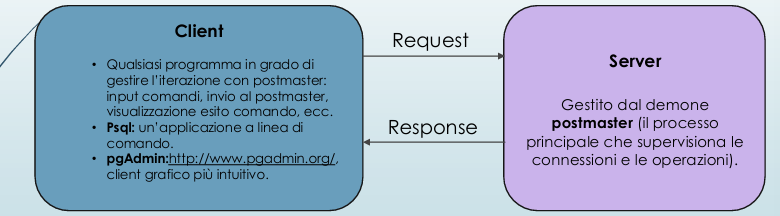
\includegraphics[width= \textwidth]{images/ClientServer.png}
    \end{figure}

    \section{Creazione di una tabella}
Struttura base
\begin{codiceSQL}
CREATE TABLE tabella (
  attributo dominio [ valoreDefault ] { vincolo }
  {, attributo dominio [ valoreDefault ] { vincolo } }
  {, vincoloTabella }
]);
\end{codiceSQL}

Costrutti inseriti: 
\begin{itemize}
  \item {[}{]} indicano parti opzionali / facoltative (il termine può non comparire o comparire una sola volta) Indica che quell'elemento può apparire zero o una volta. Sta al programmatore decidere se inserirlo o meno a seconda di ciò che si vuole ottenere)
\item {[} valoreDefault {]}: Significa che quando definisco l’attributo posso decidere se attribuirgli un valore predefinito
\item \{ \} Tutto ciò che è racchiuso tra parentesi graffe rappresenta un elemento che può essere ripetuto zero, una o più volte.
\item \{ vincolo \}: Significa che a una singola colonna puoi applicare nessun vincolo, un solo vincolo, oppure una serie di vincoli uno dopo l'altro (es. NOT NULL, UNIQUE)
\end{itemize}


\textbf{\large Ecco un esempio}
\begin{codiceSQL}
CREATE TABLE Impiegato (
  Matricola CHARACTER(6) PRIMARY KEY, 
  Nome VARCHAR(20) NOT NULL, 
  Cognome VARCHAR(20) NOT NULL,
  Dipart VARCHAR(15), 
  Stipendio NUMERIC(9) DEFAULT 0,
  FOREIGN KEY(Dipart) 
    REFERENCES Dipartimento(NomeDip),     /*vincolo di tabella*/
  UNIQUE (Cognome,Nome)                   /*vincolo di tabella*/
)
\end{codiceSQL}


\subsection{Identificatori}
 Sono stringhe che iniziano con una lettera (UTF-8) o un underscore (\_) e che possono contenere anche cifre (0-9). Gli identificatori SQL \textbf{NON} sono sensibili al minuscolo/maiuscolo:
 \begin{itemize}
  \item idPersona e idpersona rappresentano un solo identificatore.
 \end{itemize}

\subsection{Domini}
I domini elementari (predefiniti) sono:
\begin{itemize}
  \item \textbf{caratteri}: singoli caratteri o stringhe anche di lunghezza variabile
  \item \textbf{bit}: bit singoli (booleani) o stringhe di bit
  \item \textbf{numerici esatti e approssimati}
  \item \textbf{istanti temporali}
  \item \textbf{intervalli temporali}
\end{itemize}
Oppure si possono avere domini definiti dall'utente

\subsubsection{Tipo carattere}
Permette di rappresentare singoli caratteri oppure stringhe.
Un carattere o stringa di caratteri sono rappresentati tra apici (’):
’a’, ’Questa è una stringa’.\par
La lunghezza delle stringhe può essere fissa o variabile: 
\textcolor{cyan}{CHARACTER [VARYING][(lunghezza)]}
\begin{itemize}
  \item \textbf{CHARACTER}: carattere singolo
  \item \textbf{CHARACTER(20)}: stringa di \textbf{lunghezza fissa}. Se si assegna una stringa di lunghezza inferiore a 20, la stringa viene riempita di spazi fino a rendere la stringa lunga 20.
  \item \textbf{CHARACTER VARYING(20)}: stringa di \textbf{lunghezza variabile} (max 20).
  \item \textbf{TEXT}: \underline{stringa di lunghezza variabile senza limite fissato}. Questa è un’estensione PostgreSQL
\end{itemize}

\subsubsection{Tipo boolean}
Permette di rappresentare i valori booleani TRUE/FALSE, rappresentati anche 
come t/f, 1/0, yes/NO, più lo stato unknown (valore nullo), rappresentato 
come NULL

\subsubsection{Tipo numerici esatti}
Permettono di rappresentare valori esatti: interi o con una parte decimale di 
lunghezza prefissata
\begin{itemize}
  \item \textbf{Valori interi}:
\begin{itemize}
  \item SMALLINT: valori interi (2 bytes: da -32.768 (215) a +32.767 (215-1)).
  \item INTEGER: valori interi (4 bytes: da -2147483648 (231) to +2147483647 (231-1) ).
\end{itemize}
\item \textbf{Valori decimali}:
\begin{itemize}
  \item NUMERIC [(precisione [, scala])]: precisione è il numero totale di cifre  significative (cioè di cifre a sinistra e a destra della virgola), scala è il numero di cifre dopo la virgola (vuoto = 0).
\item DECIMAL [(precisione [, scala])]: equivalente al precedente.
\end{itemize}
\end{itemize}

\esempio{}{NUMERIC(5,2) permette di rappresentare valori come 100.01, 100.999 
(arrotondato a 101.00), ma non valori come 1000.01}

\subsubsection{Tipo numerici approssimati}
Permettono di rappresentare valori in virgola mobile:
\begin{itemize}
  \item \textbf{REAL}: una precisione di 6 cifre decimali.
  \item \textbf{DOUBLE PRECISION}: una precisione di 15 cifre decimali.
\end{itemize}
Ciascun numero è rappresentato da una coppia di valori: la mantissa e 
l’esponente.
\begin{itemize}
  \item La mantissa è un numero frazionario, l’esponente è un numero intero
  \item Il valore si ottiene moltiplicando la mantissa per la potenza di 10 con grado pari all’esponente
\end{itemize}
Il numero 0.17E16 corrisponde a 1,7 x 1015           
Il numero -0.4E-6 corrisponde a -4 x 10-7

\subsubsection{Istanti temporali}
Permettono di rappresentare istanti di tempo.
\begin{itemize}
  \item \textbf{DATE}: istanti del tipo (anno, mese, giorno).
  \begin{itemize}
    \item Un valore DATE si rappresenta tra apici (’) e lo standard ISO prescrive il formato \texttt{YYYY-MM-DD}.
  \end{itemize}
  \item \textbf{TIME [(precisione)][WITH TIME ZONE]}: istanti del tipo (hour, minute, second)
  \begin{itemize}
    \item precisione: numero cifre decimali per rappresentare frazioni del secondo;
    \item WITH TIME ZONE: permette di specificare anche [+-]hour:minute, che rappresentano la differenza con l’ora di Greenwich, o nomeFusoOrario.
  \end{itemize}
  \item \textbf{TIMESTAMP [(precisione)][WITH TIME ZONE]}: date + time.
\end{itemize}

\subsubsection{Intervalli temporali}
INTERVAL PrimaUnitàDiTempo[TO UltimaUnitàDiTempo]
PrimaUnitàDiTempoe UltimaUnitàDiTempodefiniscono le unità di misura che 
devono essere utilizzate, dalla più precisa alla meno precisa.
L’insieme delle unità di misura è diviso in due insiemi distinti:
\begin{itemize}
  \item Year-Month
  \item Day-Hour–Minute-Second
\end{itemize}

\subsubsection{Domini definiti dall'utente}

\begin{codiceSQL}
  CREATE DOMAIN nome AS tipoBase [valoreDefault][vincolo]
\end{codiceSQL}


\textcolor{purple}{\textbf{CREATE DOMAIN}}: definisce un dominio, utilizzabile in definizioni di relazioni, anche con 
vincoli e valori di default
Il dominio può essere definito a partire da un dominio elementare oppure da un altro 
dominio definito dall‘utente
\begin{codiceSQL}
CREATE DOMAIN giorniSettimana AS CHARACTER (3)
CHECK (VALUE IN ('LUN', 'MAR', 'MER', 'GIO', 'VEN', 'SAB', 'DOM'));
\end{codiceSQL}

\begin{codiceSQL}
CREATE DOMAIN Voto AS SMALLINT DEFAULT NULL
CHECK ( value >=18 AND value <= 30 )
\end{codiceSQL}




\subsection{Vincoli intrarelazionali}

\begin{itemize}
  \item \textbf{NOT NULL}: il valore nullo non è ammesso per l'attributo, quindi il valore deve sempre essere specificato, o si assegna un valore di default
  \item \textbf{UNIQUE}: definisce (super)chiavi
  \begin{codiceSQL}
Nome VARCHAR(20),
Cognome VARCHAR(20),
UNIQUE(Nome,Cognome)

/* impone che non ci siano due righe che abbiano uguale sia il nome che il cognome*/
  \end{codiceSQL}

  \begin{codiceSQL}
Nome VARCHAR(20) UNIQUE,
Cognome VARCHAR(20) UNIQUE

/* impone che non ci siano due righe che abbiano lo stesso nome o lo stesso cognome*/ 
  \end{codiceSQL}
  \item \textbf{PRIMARY KEY}: chiave primaria (una sola, implica NOT NULL) 
  \begin{codiceSQL}
matricola CHAR (6) PRIMARY KEY;
/* se unico componente della chiave primaria*/
  \end{codiceSQL}

  \begin{codiceSQL}
nome VARCHAR(20),
cognome VARCHAR(20),
PRIMARY KEY(nome, cognome)

/* Se la chiave primaria ha piu attributi */
  \end{codiceSQL}
  \item \textbf{CHECK}: specifica un vincolo generico che deve soddisfare le tuple della tabella. Viene soddisfatto se la sua espressione è vera o nulla.
  
\begin{codiceSQL}
CREATE TABLE Impiegato (
  matricola CHAR(6) PRIMARY KEY,
  nome VARCHAR(20) NOT NULL,
  cognome VARCHAR(20) NOT NULL,
  qualifica VARCHAR(20),
  stipendio NUMERIC(8,2) DEFAULT 500.00 NOT NULL
  CHECK( stipendio >= 0.0 ),    /* check di attributo */
  UNIQUE( cognome, nome ),
  CHECK( nome <> cognome )      /* check di tabella */
)
  \end{codiceSQL}

\end{itemize}

\subsection{Vincoli interrelazionali}
Un vincolo di integrità referenziale (= interrelazionale) crea un legame tra i 
valori di un attributo (o di un insieme di attributi) A della tabella corrente (detta interna/slave) e i valori di un attributo (o di un insieme di attributi) B di un’altra tabella (detta esterna/master):
\begin{itemize}
  \item Impone che, in ogni tupla della tabella interna, il valore di A, se diverso dal valore nullo, sia presente tra i valori di B nella tabella esterna.
  \item  L’attributo B della tabella esterna deve essere soggetto a un vincolo 
UNIQUE (o PRIMARY KEY).
\end{itemize}
\vario{Nota:}{L’attributo (o insieme di attributi) B può anche non essere la 
chiave primaria, ma deve essere identificante per le tuple della tabella 
esterna}

\textbf{REFERENCES e FOREIGN KEY permettono di definire vincoli di integrità referenziale}

Per singoli attributi, basta utilizzare il costrutto \textcolor{purple}{\textbf{REFERENCES}}
\begin{codiceSQL}
CREATE TABLE Impiegato (
  Matricola CHARACTER(6) primary key,
  Nome CHARACTER VARYING(20)  not null,
  Cognome CHARACTER VARYING(20)  not null,
  Dipart CHARACTER VARYING(15) 
  REFERENCES Dipartimento(NomeDip),   
  /* Attributo chiave (singolo) di tabella esterna*/
  Ufficio NUMERIC(3),
  Stipendio  NUMERIC(9) default 0,
  UNIQUE (Cognome, Nome)
)
\end{codiceSQL}

Per attributi multipli, si usa il costrutto \textcolor{purple}{\textbf{FOREIGN KEY}} alla fine della definizione degli attributi, seguito da \textcolor{purple}{\textbf{REFERENCES}}
\begin{codiceSQL}
CREATE TABLE Impiegato (
  Matricola CHARACTER(6) primary key,
  Nome CHARACTER VARYING(20)  not null,
  Cognome CHARACTER VARYING(20)  not null,
  Dipart CHARACTER VARYING(15),
  REFERENCES Dipartimento(NomeDip),   
  Ufficio NUMERIC(3),
  Stipendio  NUMERIC(9) default 0,
  FOREIGN KEY(Nome, Cognome)
    REFERENCES Anagrafica (Nome, Cognome) 
    /* Tabella esterna con attributi chiave*/
)
\end{codiceSQL}

Vediamo un esempio più concreto:

\begin{figure}[H]
  \centering
  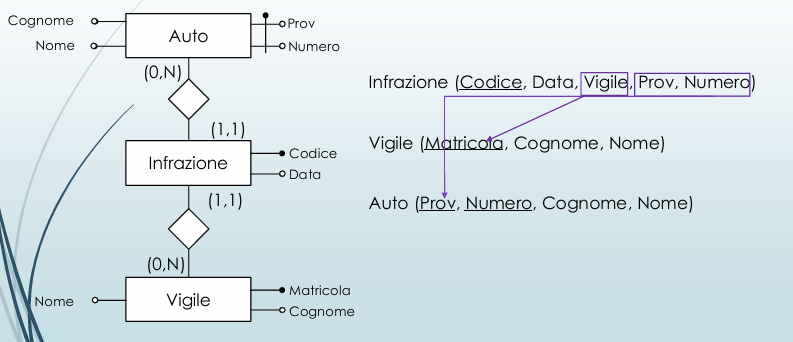
\includegraphics[width= \textwidth]{images/esempioReferences.png}
\end{figure}

\begin{codiceSQL}
CREATE TABLE Infrazione(
  Codice CHAR(6) PRIMARY KEY, 
  Data DATE NOT NULL,  
  Vigile INTEGER NOT NULL
  REFERENCES Vigile(Matricola),
  Provincia CHAR(2),  
  Numero CHAR(6) ,
  FOREIGN KEY(Provincia, Numero)
    REFERENCES Auto(Provincia, Numero)
)

\end{codiceSQL}

\section{Modifica degli schemi}
\begin{itemize}
  \item ALTER: effettua modifiche (a domini, tabelle...), ad esempio aggiungere una colonna a una relazione
  \item DROP DOMAIN: permette di rimuovere i domini
  \item DROP TABLE: cancella una tabella
\end{itemize}

\subsection{ALTER: modifiche alla struttura di una tabella}
Il costrutto \textbf{Alter} permette di:

Aggiungere un nuovo attributo (ADD COLUMN):
\begin{codiceSQL}
ALTER TABLE tabella ADD COLUMN attributo tipo;
ALTER TABLE impiegato ADD COLUMN stipendio NUMERIC(8,2);
\end{codiceSQL}

Rimuovere un attributo (DROP COLUMN):
\begin{codiceSQL}
ALTER TABLE tabella DROP COLUMN attributo;
ALTER TABLE impiegato DROP COLUMN stipendio;
\end{codiceSQL}
Modificare valore di default di un attributo (ALTER COLUMN):
\begin{codiceSQL}
ALTER TABLE tabella ALTER COLUMN attributo { SET DEFAULT valore | 
DROP DEFAULT };
ALTER TABLE impiegato ALTER COLUMN stipendio SET DEFAULT 1000.00;
\end{codiceSQL}

\section{Cancellazione dati in una tabella}
Le tuple di una tabella vengono cancellate con il comando \textcolor{purple}{\textbf{DELETE}}.
condizione è una espressione booleana che seleziona quali tuple cancellare. 
\begin{codiceSQL}
  DELETE FROM tabella [ WHERE condizione ];
\end{codiceSQL}

\vario{}{
  \textbf{Se WHERE non è presente, tutte le tuple saranno cancellate.}
}
\begin{codiceSQL}
  DELETE FROM impiegato WHERE matricola = 'A001 ';
\end{codiceSQL}

Una tabella viene cancellata con il comando \textcolor{purple}{\textbf{DROP TABLE}}:
\begin{codiceSQL}
  DROP TABLE tabella;
\end{codiceSQL}




\section{Inserimento e aggiornamento di tuple}

\textbf{\large Inserimento di valori all'interno di una tupla}

\begin{codiceSQL}
INSERT INTO Tabella [ ( Attributi ) ] 
VALUES( Valori ) 
\end{codiceSQL}
oppure
\begin{codiceSQL}
  INSERT INTO Tabella [ ( Attributi )]
(SELECT ...)
\end{codiceSQL}

\textbf{ Esempio inserimento}
\begin{codiceSQL}
INSERT INTO Museo (nome, citta, indirizzo, numeroTelefono, giornoChiusura, prezzo)
VALUES('Arena', 'Verona', 'piazza Bra', '045 8003204', 'MARTEDI', 20) 

\end{codiceSQL}


\textbf{\large Aggiornamento di valori all'interno di una tupla}

\begin{codiceSQL}
UPDATE NomeTabella
  SET Attributo = < 
  Espressione |
  SELECT ... | 
  NULL | 
  DEFAULT >
  [ WHERE Condizione ]
\end{codiceSQL}

\textbf{Esempio}
\begin{codiceSQL}
UPDATE Museo SET sitoInternet = 'www.ciao.it' WHERE citta ='Verona'  
\end{codiceSQL}


\section{Selezione}

\textbf{\large Struttura base}

\begin{codiceSQL}
SELECT [ DISTINCT ]
[ * | expression [[ AS] output_name ] [, 
...] ]
FROM from_item [, ...] 
[ WHERE condition ]
[ GROUP BY grouping_element [, ...] ]
[ HAVING condition [, ...] ]
[ { UNION | INTERSECT | EXCEPT } [ DISTINCT
] other_select ]
[ ORDER BY expression [ ASC | DESC | USING 
operator ]]

\end{codiceSQL}


\subsection{Clausola SELECT}
\begin{codiceSQL}
SELECT [ DISTINCT ]
[{* | expression [[ AS] output_name ]} [, ...]]
\end{codiceSQL}
\begin{description}
  \item [\textbf{*}] è un’abbreviazione per indicare tutti gli attributi delle tabelle.
  \item [\textbf{expression}] è un’espressione che coinvolge gli attributi della tabella (può anche essere semplicemente il nome di un attributo).
  \item [\textbf{output\_name}] è il nome assegnato all’attributo che conterrà il risultato della valutazione dell’espressione expression nella relazione risultato.
  \item [\textbf{DISTINCT}:] se presente richiede l’eliminazione delle tuple duplicate.

\end{description}


L’esecuzione di una \textbf{SELECT} produce una relazione che:
\begin{itemize}
  \item ha come schema tutti gli attributi elencati nella clausola \textbf{SELECT};
  \item ha come contenuto tutte le tuple ottenute proiettando sugli attributi 
indicati nella \textbf{SELECT} provenienti dalle tabelle del \textbf{FROM} (prodotto 
cartesiano), limitate a quelle che soddisfano le eventuali condizioni 
specificate nelle clausole \textbf{WHERE}, \textbf{GROUP BY} e \textbf{HAVING}
\end{itemize}


\subsubsection{Target List}

\begin{minipage}[t]{0.39\textwidth}
   \begin{codiceSQL}
SELECT *
FROM Tabella
   \end{codiceSQL}
\end{minipage}
\hfill % Questo comando inserisce uno spazio flessibile che spinge le due minipage ai lati opposti
\begin{minipage}[t]{0.50\textwidth}
  \vspace{1em}
   Selezione di tutti gli attributi 
delle tabelle indicate nella 
clausola FROM
\end{minipage}

\begin{minipage}[t]{0.39\textwidth}
   \begin{codiceSQL}
SELECT Attributo1, Attributo2
FROM Tabella
   \end{codiceSQL}
\end{minipage}
\hfill % Questo comando inserisce uno spazio flessibile che spinge le due minipage ai lati opposti
\begin{minipage}[t]{0.50\textwidth}
  \vspace{1em}
   Selezione di tutti gli attributi 
delle tabelle indicate nella 
clausola FROM
\end{minipage}


\textbf{Esempio}



\begin{minipage}[t]{0.39\textwidth}
 \begin{codiceSQL}
SELECT Nome, Reddito
FROM Persone
WHERE Eta < 30
\end{codiceSQL}
\end{minipage}
\hfill % Questo comando inserisce uno spazio flessibile che spinge le due minipage ai lati opposti
\begin{minipage}[t]{0.50\textwidth}
\begin{figure}[H]
  \centering
  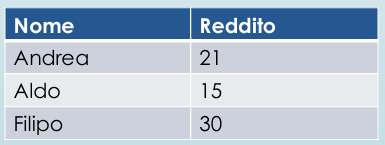
\includegraphics[width=\textwidth]{images/nomeReddito.png}
  \caption{selezionati solo le tuple dove è rispettata la condizione}
\end{figure}
\end{minipage}


\subsubsection{Concatenazione stringhe}
L'operatore di concatenazione || è un operatore scalare (o operatore di riga).

Lavora su una singola riga alla volta. Se la tua tabella ha 100 righe, il costrutto titolo || ' - ' || citta calcolerà e restituirà 100 risultati testuali separati, uno per ogni riga.

\vario{nota}{Non è un'esclusiva della SELECT}
può infatti essere utilizzato anche 

\textbf{\large Nella clausola WHERE (per filtrare i dati)}
\begin{codiceSQL}
  -- Trova la riga in cui l'unione di nome e cognome da esattamente 'Mario Rossi'
WHERE nome || ' ' || cognome = 'Mario Rossi'
\end{codiceSQL}

\textbf{\large Nella clausola ORDER BY (per ordinare i risultati)}
\begin{codiceSQL}
  -- Ordina i risultati basandosi sull'unione testuale dei due campi
ORDER BY titolo || citta
\end{codiceSQL}



\subsection{Clausola FROM}
\begin{codiceSQL}
  FROM from_item [, ...]
\end{codiceSQL}

\begin{enumerate}
  \item  table\_name [[AS] alias [(column\_alias [, ...])]]
  \begin{itemize}
    \item Se sono presenti due o più tabelle, si esegue il prodotto cartesiano tra tutte le  tabelle. Se ci sono attributi con lo stesso nome su tabelle diverse, nel SELECT 
questi attributi sono identificati anteponendo il nome della tabella e un ’.’: 
nomeTabella.nomeAttributo
  \end{itemize}

  \item  (other\_select) [AS] nomeRisultato [(column\_alias [,...])
  \begin{itemize}
    \item  è una SELECT innestata. Il risultato della SELECT interna è lo schema con nome 
nomeRisultato su cui fare la SELECT corrente.
  \end{itemize}

  \item  from\_item [NATURAL] join\_type from\_item [ON condition]
  \begin{itemize}
    \item  è la clausola JOIN.
    \item Metodo più sofisticato di 1) che permette di selezionare un sottoinsieme del 
prodotto cartesiano di due o più tabelle. join\_type specifica il tipo di join. I tipi 
principali sono riassunti nelle slide seguenti
  \end{itemize}
\end{enumerate}


\subsubsection{Uso di alias}

\begin{codiceSQL}
SELECT P.Reddito, R.Telefono
FROM Reparti as R, Persona ad P
WHERE ... ;
\end{codiceSQL}

Utile quando è necessario specificare la provenienza dell’attributo, 
perchè nella base di dati sono presenti più attributi con lo stesso nome

\subsubsection{Target List}
\begin{codiceSQL}
SELECT P.Nome as NPersona, P.Reddito as RPersona
FROM Persone as P
WHERE P.Eta < 30
\end{codiceSQL}




\subsection{Clausola WHERE}
\begin{codiceSQL}
  WHERE condition
\end{codiceSQL}

\textbf{\textcolor{black!50!red}{condition}} è un’espressione booleana combinando condizioni semplici $C_{i}$ con gli 
operatori AND, OR, NOT.
\begin{enumerate}
  \item  $C_{i}$ := expr [ $\theta$ \{expr | const\}]
dove
\begin{itemize}
  \item expr := espressione che contiene riferimenti agli attributi delle tabelle che compaiono 
nella clausola FROM.
\item $\theta \in$ \{=,<>,<,>,<=,>=\}
\item const := valore dei domini di base.
\end{itemize}
\item Una riga soddisfa \textcolor{black!50!red}{condition} se l’espressione è vera quando valutata con i valori 
della riga.
\item Una riga che non soddisfa condition è scartata dal risultato finale
\end{enumerate}





\begin{minipage}[t]{0.39\textwidth}
 \begin{codiceSQL}
SELECT Nome, Reddito
FROM Persone
WHERE Eta < 30;
\end{codiceSQL}
\end{minipage}
\hfill % Questo comando inserisce uno spazio flessibile che spinge le due minipage ai lati opposti
\begin{minipage}[t]{0.50\textwidth}
SELECT Nome, Reddito
FROM Persone
WHERE Età < 30 OR Reddito > 50;
\end{minipage}




\subsubsection{Operatore LIKE}
\begin{codiceSQL}
WHERE attributo [NOT] LIKE 'pattern';
\end{codiceSQL}

Nella clausola WHERE può apparire l’operatore LIKE per il confronto di stringhe. 
LIKE è un operatore di pattern matching. I pattern si costruiscono con i 
caratteri speciali \_ e \%:
\begin{itemize}
  \item \_ = 1 carattere qualsiasi.
  \item \% = 0 o più caratteri qualsiasi.
\end{itemize}


\begin{minipage}[t]{0.39\textwidth}
  \vspace{2em}
  \begin{codiceSQL}
SELECT Nome,Reddito
FROM Persona
WHERE Nome LIKE 'A\%a'
  \end{codiceSQL}
\end{minipage}
\hfill 
\begin{minipage}[t]{0.50\textwidth}
  \vspace{0pt}
  % Rimosso totalmente \begin{figure}[H] e \end{figure}
  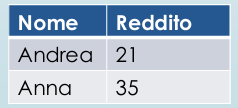
\includegraphics[width=0.8\textwidth]{images/nomeReddito2.png}
\end{minipage}  


\subsubsection{Operatore SIMILAR TO}


L’operatore \textbf{\textcolor{purple}{SIMILAR TO}} è un \textbf{\textcolor{purple}{LIKE}} più espressivo che accetta, come pattern, 
un sottoinsieme delle espressioni regolari POSIX (versione SQL). 
Esempi di componenti di espressioni regolari:
\begin{itemize}
  \item \_ = 1 carattere qualsiasi. 
  \item \% = 0 o più caratteri qualsiasi.
  \item * = ripetizione del precedente match 0 o più volte.
  \item + = ripetizione del precedente match UNA o più volte.
  \item \{n,m\} = ripetizione del precedente match almeno n e non più di m volte.
  \item {[} ... {]} = ... è un elenco di caratteri ammissibili
\end{itemize}


\begin{minipage}[t]{0.50\textwidth}
  \vspace*{0pt}
  \begin{codiceSQL}[unbreakable]
SELECT *
FROM Persone
WHERE Nome SIMILAR TO '[AFO]'
  \end{codiceSQL}
\end{minipage}
\hfill 
\begin{minipage}[t]{0.45\textwidth}
  \vspace*{0pt}
  \vspace{1.5em} % Spazio per allineare il testo al centro del codice
Per trovare nomi che inziano per A,F o O
\end{minipage}  


\subsubsection{Operatore BETWEEN}

\begin{codiceSQL}
WHERE attributo [NOT] BETWEEN valore_iniziale AND valore_finale;
\end{codiceSQL}

Nella clausola \textcolor{purple}{\textbf{WHERE}} può apparire l’operatore \textcolor{purple}{\textbf{BETWEEN}} per testare l’appartenenza 
di un valore ad un intervallo (non limitato ai valori numerici, usato anche con date e 
stringhe)


\begin{minipage}[t]{0.40\textwidth}
  \begin{codiceSQL} 
SELECT *
FROM Persone
WHERE Eta BETWEEN 20 AND 40
  \end{codiceSQL}
\end{minipage}
\hfill 
\begin{minipage}[t]{0.45\textwidth}
  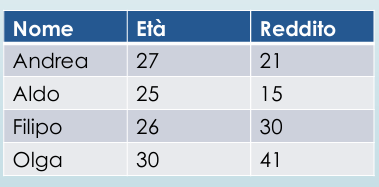
\includegraphics[width=0.8\textwidth, valign=t]{images/nomeEtaReddito.png}
\end{minipage}


\subsubsection{Operatore IN}
\begin{codiceSQL}
  WHERE attributo [NOT] IN ( valore [, ...] );

\end{codiceSQL}
Nella clausola WHERE può apparire l’operatore [\textbf{\textcolor{purple}{NOT}}] \textbf{\textcolor{purple}{IN}} per testare 
l’appartenenza di un valore ad un insieme.
\begin{codiceSQL}
SELECT *
FROM Persone
WHERE Nome NOT IN ('Andrea', 'Franco')
\end{codiceSQL}

\subsubsection{Operatore IS NULL}
\begin{codiceSQL}
WHERE attributo IS [ NOT ] NULL;
\end{codiceSQL}
Nella clausola WHERE può apparire l’operatore \textbf{\textcolor{purple}{IS}} [\textbf{\textcolor{purple}{NOT}}] \textbf{\textcolor{purple}{NULL}} per testare se un 
valore è \textbf{\textcolor{purple}{NOT KNOWN (NULL)}} o no.
Il valore NULL non rappresenta lo zero o una stringa vuota, ma l'assenza di dati 
o un valore sconosciuto.
A partire dalle versioni SQL-2 è stata adottata una logica a tre valori (true, 
false, unknown) e i valori nulli non sono considerati né veri, né falsi.\par
\begin{center}
NON SI PUÒ usare ’=’ o ’<>’ con il valore NULL!  
\end{center}

\begin{codiceSQL}
SELECT *
FROM Persone
WHERE Reddito IS NOT NULL
\end{codiceSQL}

\subsubsection{Operatore ORDER BY}
\begin{codiceSQL}
  ORDER BY attributo [{ ASC | DESC }] [, ... ];
\end{codiceSQL}
La clausola ORDER BY ordina le tuple del risultato in ordine rispetto agli attributi 
specificati,
ASCendente è lo standard.
\begin{codiceSQL}
SELECT Nome
FROM Persone
ORDER BY Nome DESC

\end{codiceSQL}

\subsubsection{Operatori di aggregazione}


Sono operatori che permettono di determinare un valore considerando i valori 
ottenuti da una SELECT.
Due tipi principali:
\begin{itemize}
  \item COUNT.
  \item MAX, MIN, AVG, SUM.
\end{itemize}

\begin{codiceSQL}
SELECT MAX(Reddito) 
FROM Persone;
\end{codiceSQL}

\vario{Nota}{Quando si usano gli operatori aggregati, dopo la SELECT non possono 
comparire espressioni che usano i valori presenti nelle singole tuple perché il 
risultato è sempre e solo una tupla
}



  \begin{enumerate}
    \item \textbf{Count}
    \begin{codiceSQL}
      COUNT({ *| expr | ALLexpr | DISTINCTexpr }])
    \end{codiceSQL}
    Restituisce il numero di tuple significative nel risultato dell’interrogazione.
    Tre casi comuni:\begin{itemize}
      \item \textcolor{purple}{COUNT(*)} ritorna il numero di tuple nel risultato dell’interrogazione.
      \item \textcolor{purple}{COUNT(expr)} ritorna il numero di tuple in ciascuna delle quali il valore expr è non nullo
      \item \textcolor{purple}{COUNT(ALL expr)} include duplicati e valori nulli.
      \item \textcolor{purple}{COUNT(DISTINCT expr)} come con \textcolor{purple}{COUNT(expr)} ma con l’ulteriore condizione che i valori di expr siano distinti
    \end{itemize}
    \item \textbf{SUM/MAX/MIN/AVG} 
    \begin{codiceSQL}
      op ({ expr | DISTINCTexpr })
    \end{codiceSQL}
    Determinano un valore numerico (SUM/AVG) o alfanumerico (MAX/MIN) considerando le tuple significative nel risultato dell’interrogazione.
    \begin{itemize}
      \item op = SUM | AVG | MAX | MIN;
      \item expr è un’espressione che usa uno o più attributi e funzioni di attributi.
      \item DISTINCT considero solo i valori distinti.  
    \end{itemize}
    \begin{codiceSQL}
      SELECT AVG(Eta) AS Media\_Eta
      FROM Persone;
    \end{codiceSQL}
  \end{enumerate}


  \section{Esempi di interrogazioni}
  \subsection{Interrogazione con raggruppamento: Group by}

  Un raggruppamento è un insieme di tuple che hanno medesimi valori su uno o più attributi caratteristici del raggruppamento.\par
La clausola GROUP BY attr [, ...] permette di determinare tutti i raggruppamenti delle tuple della relazione risultato (tuple selezionate con la clausola WHERE) in funzione degli attributi dati.\par
In una interrogazione che usa GROUP BY, la clausola SELECT contiene solamente gli attributi (da 0 a tutti) utilizzati per il raggruppamento ed eventuali funzioni di aggregazione sugli altri attributi.


\textbf{\large Visualizzare tutte le città raggruppate della tabella Studente}
\begin{codiceSQL}
SELECT citta
FROM studente
GROUP BY citta
\end{codiceSQL}

\noindent
\begin{minipage}[t]{0.6\textwidth}
   \centering
   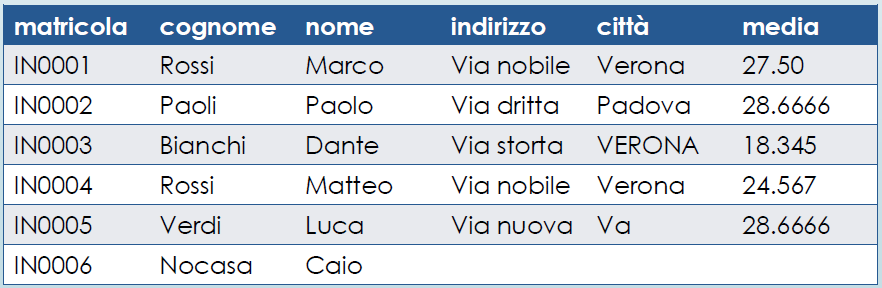
\includegraphics[width = 0.8\textwidth]{images/TableALL.png} 
\end{minipage}
\hfill % Questo comando inserisce uno spazio flessibile che spinge le due minipage ai lati opposti
\begin{minipage}[t]{0.38\textwidth}
   \centering
   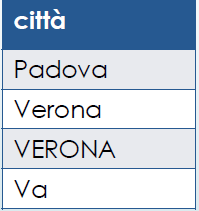
\includegraphics[width = 0.4\textwidth]{images/Group_By.png} 
\end{minipage}




\textbf{\large Visualizzare tutte le città e i cognomi raggruppati}




\noindent
\begin{minipage}{0.5\textwidth}
   \begin{codiceSQL}
SELECT cognome,LOWER(citta)
FROM Studente
GROUP BY cognome,LOWER(citta);
   \end{codiceSQL}
\end{minipage}
\hfill % Questo comando inserisce uno spazio flessibile che spinge le due minipage ai lati opposti
\begin{minipage}[t]{0.40\textwidth}
   \centering
   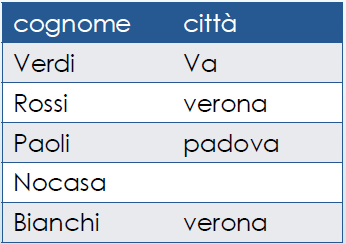
\includegraphics[width = 0.5\textwidth]{images/tabellaRisultante.png} 
\end{minipage}




\vario{Nota}{Nel GROUP BY non si possono usare espressioni con operatori di aggregazione.}

\vario{Nota}{Nella SELECT con GROUP BY non si possono specificare attributi che non sono raggruppati.}



\begin{itemize}
  \item La clausola WHERE permette di selezionare le righe che devono far parte del risultato.
  \item La clausola HAVING permette di selezionare i raggruppamenti che devono far parte del risultato.
  \item La sintassi è HAVING bool\_expr, dove bool\_expr è un’espressione booleana che può usare gli attributi usati nel GROUP BY e/o gli altri attributi mediante operatori di aggregazione.
\end{itemize}


\textbf{\large Visualizzare tutte le città raggruppate che iniziano con ’V’ della tabella Studente.}



\noindent
\begin{minipage}{0.5\textwidth}
   \begin{codiceSQL}
SELECT citta
FROM Studente
GROUP BY citta
HAVING citta LIKE 'V%';
   \end{codiceSQL}
\end{minipage}
\hfill % Questo comando inserisce uno spazio flessibile che spinge le due minipage ai lati opposti
\begin{minipage}[t]{0.40\textwidth}
   \centering
   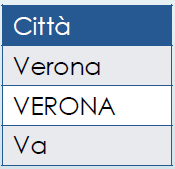
\includegraphics[width = 0.5\textwidth]{images/tabellaRisultante2.png} 
\end{minipage}




\textbf{\large Visualizzare tutte le città e i cognomi raggruppati con almeno due studenti con lo stesso cognome..}



\noindent
\begin{minipage}{0.5\textwidth}
   \begin{codiceSQL}
SELECT cognome, LOWER(citta)
FROM Studente
GROUP BY cognome, LOWER(citta)
HAVING COUNT ( cognome) >1;
   \end{codiceSQL}
\end{minipage}
\hfill % Questo comando inserisce uno spazio flessibile che spinge le due minipage ai lati opposti
\begin{minipage}[t]{0.40\textwidth}
   \centering
   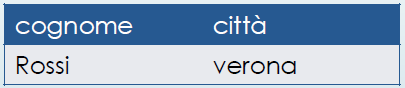
\includegraphics[width = 0.5\textwidth]{images/tabellaRisultante3.png} 
\end{minipage}



\textbf{\large Si possono specificare espressioni con operatori di aggregazione su attributi non raggruppati anche nella clausola HAVING.}



\noindent
\begin{minipage}{0.5\textwidth}
   \begin{codiceSQL}
SELECT LOWER(citta) AS "Citta", AVG (media)::DECIMAL(5 ,2) AS "mediaArr."
FROM Studente
GROUP BY LOWER(citta)
HAVING AVG(media) >23.47 ;
   \end{codiceSQL}
\end{minipage}
\hfill % Questo comando inserisce uno spazio flessibile che spinge le due minipage ai lati opposti
\begin{minipage}[t]{0.40\textwidth}
   \centering
   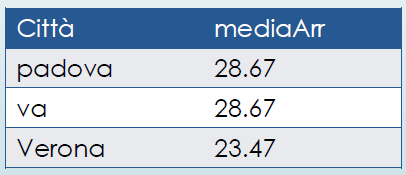
\includegraphics[width = 0.5\textwidth]{images/tabellaRisultante4.png} 
\end{minipage}



\subsection{Interrogazione con JOIN}

\begin{codiceSQL}
  TABLE1 join_typeTABLE2 ON join_condition[, ...].
\end{codiceSQL}


\textcolor{cyan}{INNER JOIN}, \textcolor{cyan}{LEFT [OUTER] JOIN}, \textcolor{cyan}{RIGHT [OUTER] JOIN} e \textcolor{cyan}{FULL [OUTER] JOIN}.
Dove \textcolor{cyan}{join\_condition} è un’espressione booleana che seleziona le tuple del join da aggiungere al risultato.
Le tuple selezionate possono essere poi filtrate con la condizione della clausola \textcolor{purple}{WHERE}.
Il prodotto cartesiano di due o più tabelle è un \textcolor{cyan}{CROSS JOIN}.


\textbf{\large Interrogazioni con INNER JOIN
Rappresenta}

\begin{codiceSQL}
  table1 [ INNER] JOIN table2 ON join_condition[, ...]
\end{codiceSQL}


Rappresenta il tradizionale $\theta$ join dell’algebra relazionale.
Combina ciascuna riga r1 di table1 con ciascuna riga di table2 che soddisfa la condizione della clausola ON.
table1 [ INNER] JOIN table2 ON join\_condition[, ...]



\subsection{Interrogazioni con LEFT OUTER JOIN}
\begin{codiceSQL}
  table1 LEFT[ OUTER] JOIN table2 ON join_condition[, ...].
\end{codiceSQL}

Si esegue un INNER JOIN. Poi, per ciascuna riga r1 di table1 che non soddisfa la condizione con qualsiasi riga di table2, si aggiunge una riga al risultato con i valori di r1 e assegnando NULL agli altri attributi..

Il LEFT [OUTER] JOIN non è simmetrico!
Con le medisime tabelle si possono ottenere risultati diversi invertendo l’ordine delle tabelle nel join!


\subsection{Interrogazioni con RIGHT OUTER JOIN}

\begin{codiceSQL}
  table1 RIGHT[ OUTER] JOIN table2 ON join_condition[, ...].
\end{codiceSQL}

Si esegue un INNER JOIN. Poi, per ciascuna riga r2 di table2 che non soddisfa la condizione con qualsiasi riga di table1, si aggiunge una riga al risultato con i valori di r2 e assegnando NULL agli altri attributi..


\subsection{Interrogazioni con FULL OUTER JOIN}

\begin{codiceSQL}
  table1 FULL[ OUTER] JOIN table2 ON join\_condition[, ...].
\end{codiceSQL}

\begin{itemize}
  \item È equivalentea:INNER JOIN + LEFT OUTER JOIN + RIGHT OUTER JOIN.
  \item \textcolor{black!60!red}{Non è equivalentea CROSS JOIN!}
\end{itemize}


  \section{Interrogazioni nidificate e insiemistiche}

  \subsection*{Interrogazioni nidificate}
  SQL permette la costruzione di interrogazioni che presentano al loro interno altre interrogazioni. 
La nidificazione può avvenire nelle clausole \textcolor{purple}{SELECT}, \textcolor{purple}{FROM}, \textcolor{purple}{WHERE}.
L'uso più comune è la nidificazione nella clausola WHERE

\subsection{Clausola FROM}
Con l'utilizzo di questa opzione, è possibile comporre catene di interrogazioni, 
in cui ciascuna interrogazione utilizza il risultato della precedente come se 
fosse una tabella di base

\begin{codiceSQL}
  SELECT titolo, prezzoIntero
FROM Mostra, ( SELECT MAX ( prezzoIntero ) 
FROM Mostra ) AS T( prezzoMax )
WHERE prezzoIntero = prezzoMax;
\end{codiceSQL}

\subsection{Clausola WHERE}
Il predicato (predicato complesso) nella clausola WHERE confronta un valore (ottenuto come espressione valutata sulla singola riga), con il risultato dell'esecuzione di un'interrogazione SQL (in generale un insieme di valori). 
Occorre estendere gli operatori di confronto per poter realizzare la comparazione tra un valore e un insieme di valori



Soluzione offerta da SQL: estensione degli operatori di confronto (>,<, =, <=, 
>=, <>) con ANY/SOME e ALL (IN, NOT IN). 
\begin{itemize}
  \item \textcolor{purple}{ANY/SOME}: specifica che la riga soddisfa la condizione se risulta vero il 
confronto (con l'operatore specificato) tra il valore dell'attributo per la riga e 
\textbf{almeno uno} degli elementi restituiti dall'interrogazione. 
  \item \textcolor{purple}{ALL}: specifica che la riga soddisfa la condizione solo se \textbf{tutti gli elementi} 
restituiti dall'interrogazione nidificata rendono vero il confronto. 
\item \textcolor{purple}{IN} e \textcolor{purple}{NOT IN}: usati per rappresentare l'appartenenza o l'esclusione rispetto ad 
un insieme (identici a = ANY o <>ALL)
\end{itemize}


\subsubsection{Operatore ANY/SOME}
\begin{codiceSQL}
  expression operator ANY( subquery )
expression operator SOME( subquery )
\end{codiceSQL}

\begin{itemize}
  \item \textcolor{orange}{expression} è un’espressione che coinvolge attributi della SELECT principale.
  \item (\textcolor{orange}{subquery}) è una \textcolor{purple}{SELECT} che deve restituire UNA sola colonna;
  \item \textcolor{orange}{operator} è un operatore di confronto, come ’=’, ’>=’, ...
  \item \textcolor{purple}{ANY} :è vero se la condizione è vera per almeno un valore della subquery.
  \item \textcolor{purple}{SOME} è uno sinonimo di \textcolor{purple}{ANY}
\end{itemize}


\textbf{\large Visualizzare il nome degli insegnamenti che hanno un numero di crediti 
inferiore alla media dell’ateneo di un qualsiasi anno accademico.}

\begin{codiceSQL}
  SELECT DISTINCT I.nomeins , IE.crediti
FROM Insegn I JOIN InsErogato IE ON I.id=IE.id_insegn
WHERE IE.crediti < ANY (
SELECT AVG ( crediti ) FROM InsErogato
WHERE modulo =0
GROUP BY annoaccademico
);
\end{codiceSQL}


\subsubsection{Operatore ALL}
\begin{codiceSQL}
  expression operator ALL( subquery )
\end{codiceSQL}

\begin{itemize}
  \item  \textcolor{orange}{expression} è un’espressione che coinvolge attributi della SELECT principale.
  \item (\textcolor{orange}{subquery}) è una \textcolor{purple}{SELECT} che deve restituire UNA sola colonna;
  \item \textcolor{orange}{operator} è un operatore di confronto, come ’=’, ’>=’, ...
  \item \textcolor{purple}{ALL}: La condizione è vera solo se è vera per TUTTI i valori della subquery.

\end{itemize}

\textbf{\large Trovare il nome degli insegnamenti con almeno un docente e crediti maggiori rispetto ai 
crediti di ciascun insegnamento del corso di laurea con id=6. (si considerano solo 
occorrenze insegnamento genitore)}

\begin{codiceSQL}
  SELECT DISTINCT I. nomeins , IE. crediti
FROM Insegn I JOIN InsErogato IE ON I.id = IE. id_insegn
JOIN Docenza D ON IE.id = D. id_inserogato
WHERE IE. modulo = 0 AND IE. crediti > ALL (
SELECT crediti FROM InsErogato
WHERE id_corsostudi = 6 AND modulo =0
);
\end{codiceSQL}

\subsubsection{Operatore IN}
E’ un operatore utilizzabile nei predicati complessi.
\begin{codiceSQL}
\[ROW\]( expr \[ ,...\]) IN ( subquery )  
\end{codiceSQL}
\begin{itemize}
  \item \textcolor{orange}{expr} è un’espressione costruita con un attributo della query principale. Ci 
possono essere una o più espressioni.
\item La (\textcolor{orange}{subquery}) deve restituire un numero di colonne pari al numero di 
espressioni in (\textcolor{orange}{expr} [,...]).
\item I valori dell’espressioni vengono confrontati con i valori di ciascuna riga del 
risultato di (subquery).
\item Il confronto ritorna vero se i valori sono uguali ai valori di almeno una riga della 
subquery.
\end{itemize}



\textbf{\large Trovare gli impiegati che hanno stesso nome e cognome di qualcuno in 
un’altra azienda.}
\begin{codiceSQL}
SELECT I.nome , I.cognome
FROMImpiegato I
WHERE ROW( I.nome , I.cognome ) IN (
SELECT I1.nome, I1. cognome FROM ImpiegatoAltraAzienda I1
)
\end{codiceSQL}



\subsubsection{Operatore EXIST}
E’ una clausola utilizzabile nei predicati complessi
\begin{codiceSQL}
  EXISTS(subquery)
\end{codiceSQL}


\begin{itemize}
  \item (subquery) è una \textcolor{purple}{SELECT}.
  \item \textcolor{purple}{EXISTS} ritorna falso se (subquery) non contiene righe; altrimenti vero.
  \item \textcolor{purple}{EXISTS} è significativo quando nella (subquery) si selezionano righe usando i 
valori della riga corrente nella \textcolor{purple}{SELECT} principale: \textcolor{red}{data binding. Vale a dire 
se subquery è un'interrogazione dipendente dalla query esterna}
\end{itemize}


\textbf{\large Determinare i nomi degli impiegati che sono diversi tra loro ma di pari 
lunghezza}

\begin{codiceSQL}
  SELECT I. nome
FROM Impiegato I
WHERE EXISTS (
SELECT 1 FROM Impiegato I1 WHERE I.nome <> I1. nome
AND CHAR_LENGTH( I.nome ) = CHAR_LENGTH( I1. nome )
)
\end{codiceSQL}
I.nome nella subquery è il valore di nome nella riga corrente della SELECT 
principale


\vario{Nota }{Se si usano attributi esterni nella subquery (data binding), la subquery
deve essere valutata per ogni riga della SELECT principale}


\textbf{\large Visualizzare il nome e il cognome dei docenti, escludendo i coordinatori, che hanno 
tenuto almeno due insegnamenti (o moduli) con più di 24 crediti nel 2010/2011}

\begin{codiceSQL}
  SELECT P.nome , P.cognome
FROM Persona P
WHERE EXISTS (
SELECT 1 FROM Docenza D JOIN InsErogato IE ON D. id_inserogato = IE.id
WHERE IE. crediti > 24 AND D. coordinatore = '0'
AND IE. annoaccademico = '2010/2011' AND D. id_persona = P.id
GROUP BY D. id_persona
HAVING COUNT (*) >=2
);

\end{codiceSQL}

\textbf{\large Visualizzare il nome dei corsi di studio che nel 2006/2007 non
hanno 
erogato insegnamenti il cui nome contiene la sottostringa ’Info’.}


\begin{codiceSQL}
  SELECT CS. nome FROM CorsoStudi CS
WHERE NOT EXISTS (
SELECT 1 FROM InsErogato IE JOIN Insegn I ON IE. id_insegn = 
I.id
WHERE I.nomeins LIKE '%Info%'
AND IE.annoaccademico = '2006/2007'
AND IE.id_corsostudi = CS.id)
\end{codiceSQL}



\subsection*{Interrogazioni di tipo insiemistico}

\begin{codiceSQL}
  query_1 { UNION | INTERSECT | EXCEPT } [ALL] query_2
\end{codiceSQL}

SQL mette a disposizione anche degli operatori insiemistici UNION, INTERSECT e 
EXCEPT per manipolare i risultati di più query.
Gli operatori insiemistici si possono utilizzare solo al livello più esterno di una 
query, operando sul risultato di due o più clausole SELECT.
Si possono avere sequenze di UNION/INTERSECT/EXCEPT


Gli operatori si possono applicare solo quando \textcolor{cyan}{query1} e \textcolor{cyan}{query2} producono 
risultati con lo stesso numero di colonne e di tipo compatibile fra loro.
Tutti gli operatori eliminano i duplicati dal risultato a meno che ALL non sia 
stato specificato.
\begin{itemize}
  \item \textcolor{red}{UNION} aggiunge il risultato di \textcolor{cyan}{query2} a quello di \textcolor{cyan}{query1}.
  \item \textcolor{red}{INTERSECT} restituisce le righe che sono presenti sia nel risultato di \textcolor{cyan}{query1} sia in quello di \textcolor{cyan}{query2}
  \item \textcolor{red}{EXCEPT} restituisce le righe di \textcolor{cyan}{query1} che non sono presenti nel risultato di \textcolor{cyan}{query2}. In pratica esegue la differenza insiemistica


\end{itemize}


\textbf{\large Visualizzare i nomi degli insegnamenti e i nomi dei corsi di laurea 
che non iniziano per 'A' mantenendo i duplicati}

\begin{codiceSQL}
  SELECT nomeins
FROM Insegn
WHERE NOT nomeins LIKE 'A%'
UNION ALL
SELECT nome
FROM CorsoStudi
WHERE NOT nome LIKE 'A%'
\end{codiceSQL}

    
\textbf{\large
  Visualizzare i nomi degli insegnamenti che sono anche nomi 
di corsi di laurea.
}

\begin{codiceSQL}
  SELECT nomeins
FROM Insegn
INTERSECT ALL
SELECT nome
FROM CorsoStudi;
\end{codiceSQL}

\textbf{\large Visualizzare i nomi degli insegnamenti che NON sono anche 
nomi di corsi di laurea.}

\begin{codiceSQL}
  SELECT nomeins
FROM Insegn
EXCEPT
SELECT nome
FROM CorsoStudi;
\end{codiceSQL}

\subsection{Le viste}

Le viste sono tabelle virtuali il cui contenuto dipende dal contenuto delle altre 
tabelle della base di dati.
In SQL le viste vengono definite associando un nome ed una lista di attributi al 
risultato dell’esecuzione di un’interrogazione.
\textcolor{purple}{Ogni volta che si usa una vista, si esegue la query che la definisce.}
Nell’interrogazione che definisce la vista possono comparire anche altre viste.
SQL \textcolor{red}{non ammette} però
\begin{itemize}
  \item  dipendenze immediate (definire una vista in termini di se stessa) o ricorsive 
(definire una interrogazione di base e una interrogazione ricorsiva);
\item dipendenze transitive circolari (V1 definita usando V2, V2 usando V3,. . . , Vn
usando V1).
\end{itemize}

\begin{codiceSQL}
  CREATE [ TEMP ] VIEW nome [( col_name [, ...]) ] AS query

\end{codiceSQL}

\textcolor{purple}{TEMP}: la vista è temporanea. Quando ci si sconnette, la vista viene distrutta. È 
un’estensione di PostgreSQL. Nella base di dati did2014 si possono fare solo 
viste temporanee

\begin{itemize}
  \item  \textcolor{cyan}{column\_name}: nomi delle colonne che compongono la vista; se non 
vengono specificati, sono ricavati dai nomi delle colonne restituiti dalla 
query, eventualmente tramite alias.
\item \textcolor{cyan}{query} deve restituire un insieme di attributi pari e nel medesimo ordine a 
quello specificato con ( \textcolor{cyan}{column\_name} [, ...] ) se presente.
\item SQL permette che una vista sia aggiornabile solo quando ciascuna tupla
della vista corrisponde a una sola tupla di ciascuna tabella di base.

\end{itemize}


\textbf{\large efinire la vista che contiene gli insegnamenti erogati completi di nomeins e codiceins
presi dalla tabella Insegn.}

\begin{codiceSQL}
  CREATE TEMP VIEW InsErogatiCompleti AS
SELECT I. nomeins , I. codiceins , IE .*
FROM InsErogato IE
JOIN Insegn I ON IE. id_insegn = I.id;
\end{codiceSQL}


\textbf{\large Si vuole determinare quali sono i corsi di studi con il massimo numero di nome di insegnamenti 
diversi}

Prima si crea una vista:
\begin{codiceSQL}
  CREATE TEMP VIEW InsCorsoStudi (Nome , NumIns) AS
SELECT CS.nome , COUNT ( DISTINCT I. nomeins )
FROM CorsoStudi CS
JOIN InsErogato IE ON CS.id=IE. id_corsostudi
JOIN Insegn I ON IE. id_insegn = I.id 
GROUP BY CS.nome;

\end{codiceSQL}

Poi la si usa:

\begin{codiceSQL}
  SELECT Nome, NumIns
FROM InsCorsoStudi
WHERE NumIns = ANY (
SELECT MAX ( NumIns ) FROM InsCorsoStudi);
\end{codiceSQL}

Laurea specialistica in Medicina e Chirurgia: 320


ora come dicevo marco succhia il bannano a tutti

%\includeonly{capitolo2} usando questo comando nel preambolo viene compilato solo la parte di interesse avendo però in memoria gli indici etc..

  \end{document} 